% !TEX encoding = UTF-8 Unicode 
% !TEX root = praca.tex

\chapter{Implementation of sample applications}

In this chapter, the development of the sample applications is presented. The implementation is based on the research scenarios defined in chapter \ref{chap:research_scenarios}.

\section{Research scenario 1: List scrolling and filtering}

The application consists of two main elements: a \emph{Switch} and a \emph{List}. Toggling the \emph{Switch} applies filtering (only every 6th element remains). The \emph{List} is generated automatically with 10000 elements and is scrollable. The optimal components (e.g. Flutter's \emph{ListView.builder}) have been chosen per each technology, therefore only visible items are rendered.

\begin{figure}[H]
    \begin{minipage}{.47\textwidth}
      \centering
      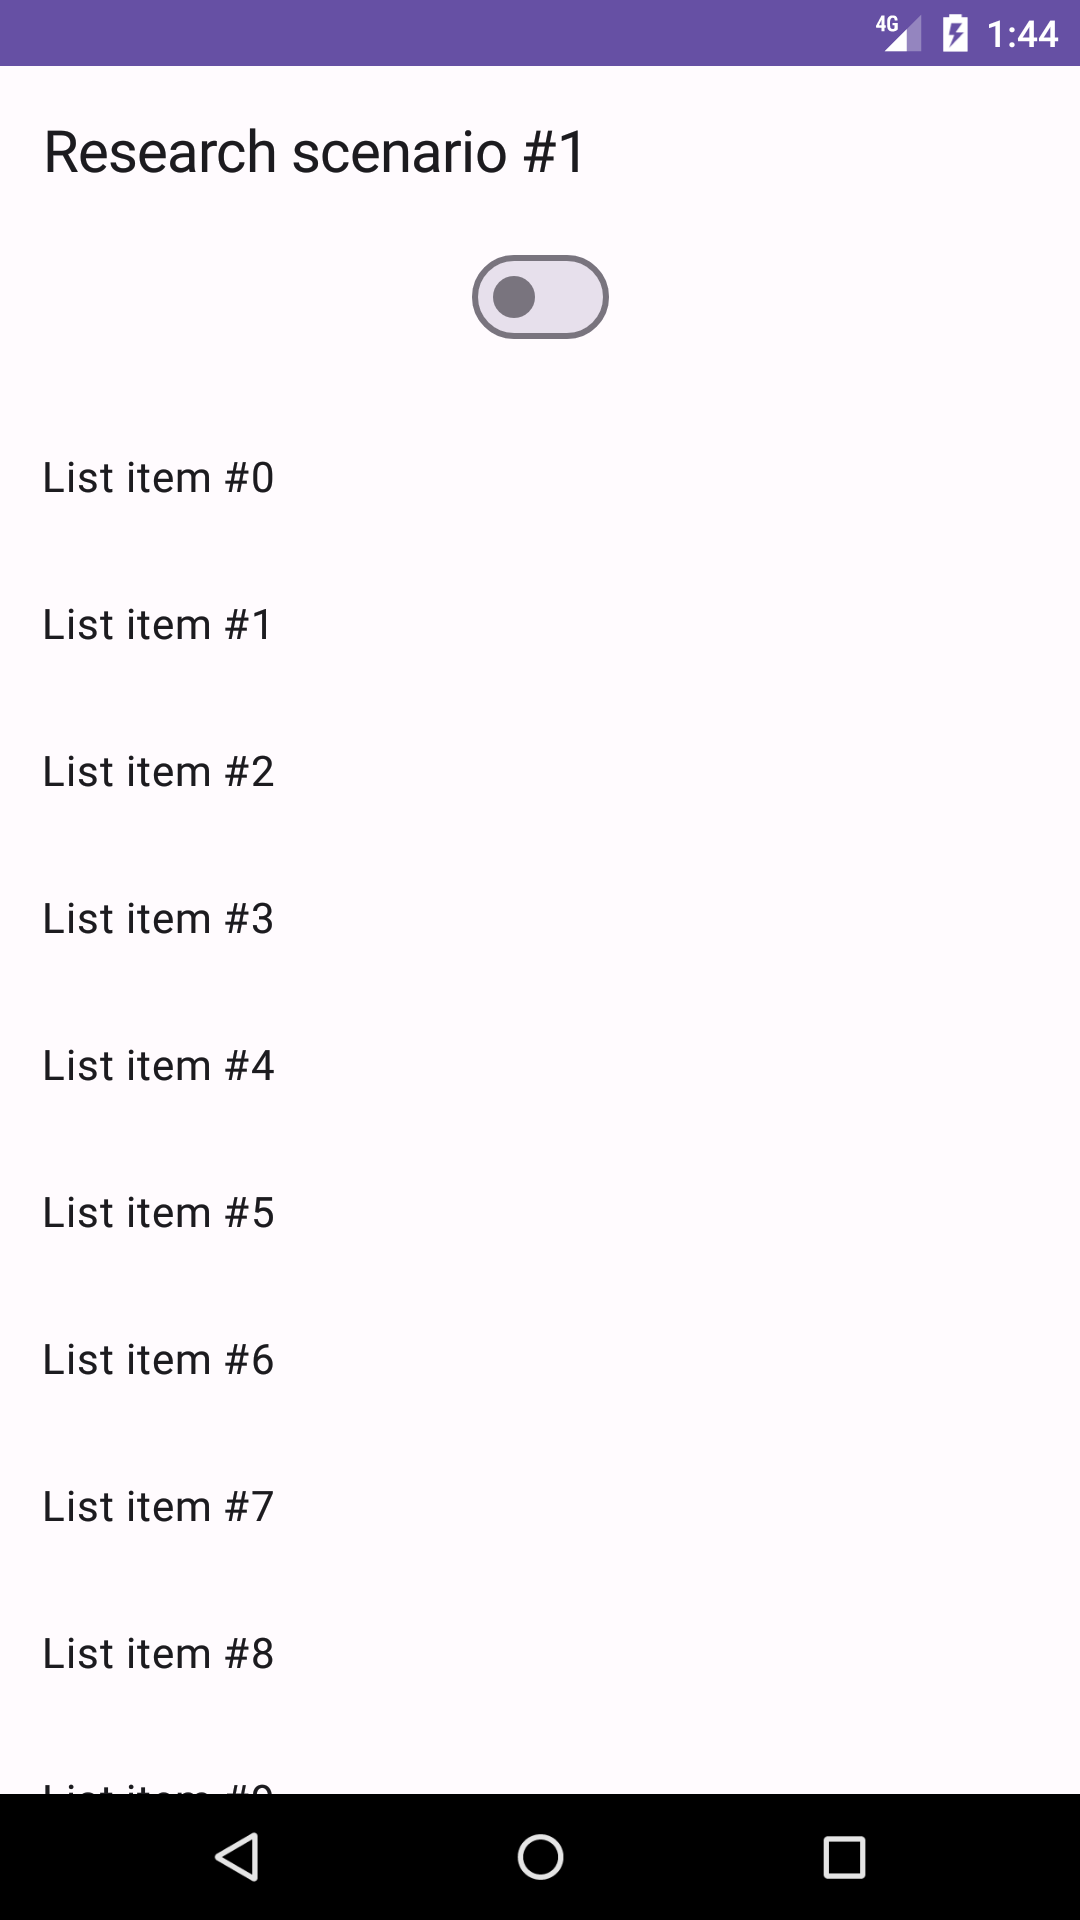
\includegraphics[height=50mm]{img/app1_kotlin}
      \caption{App 1: Kotlin (Source: Own work)}
      \label{fig:app1_kotlin}
    \end{minipage}
    \hfill
    \begin{minipage}{.47\textwidth}
      \centering
      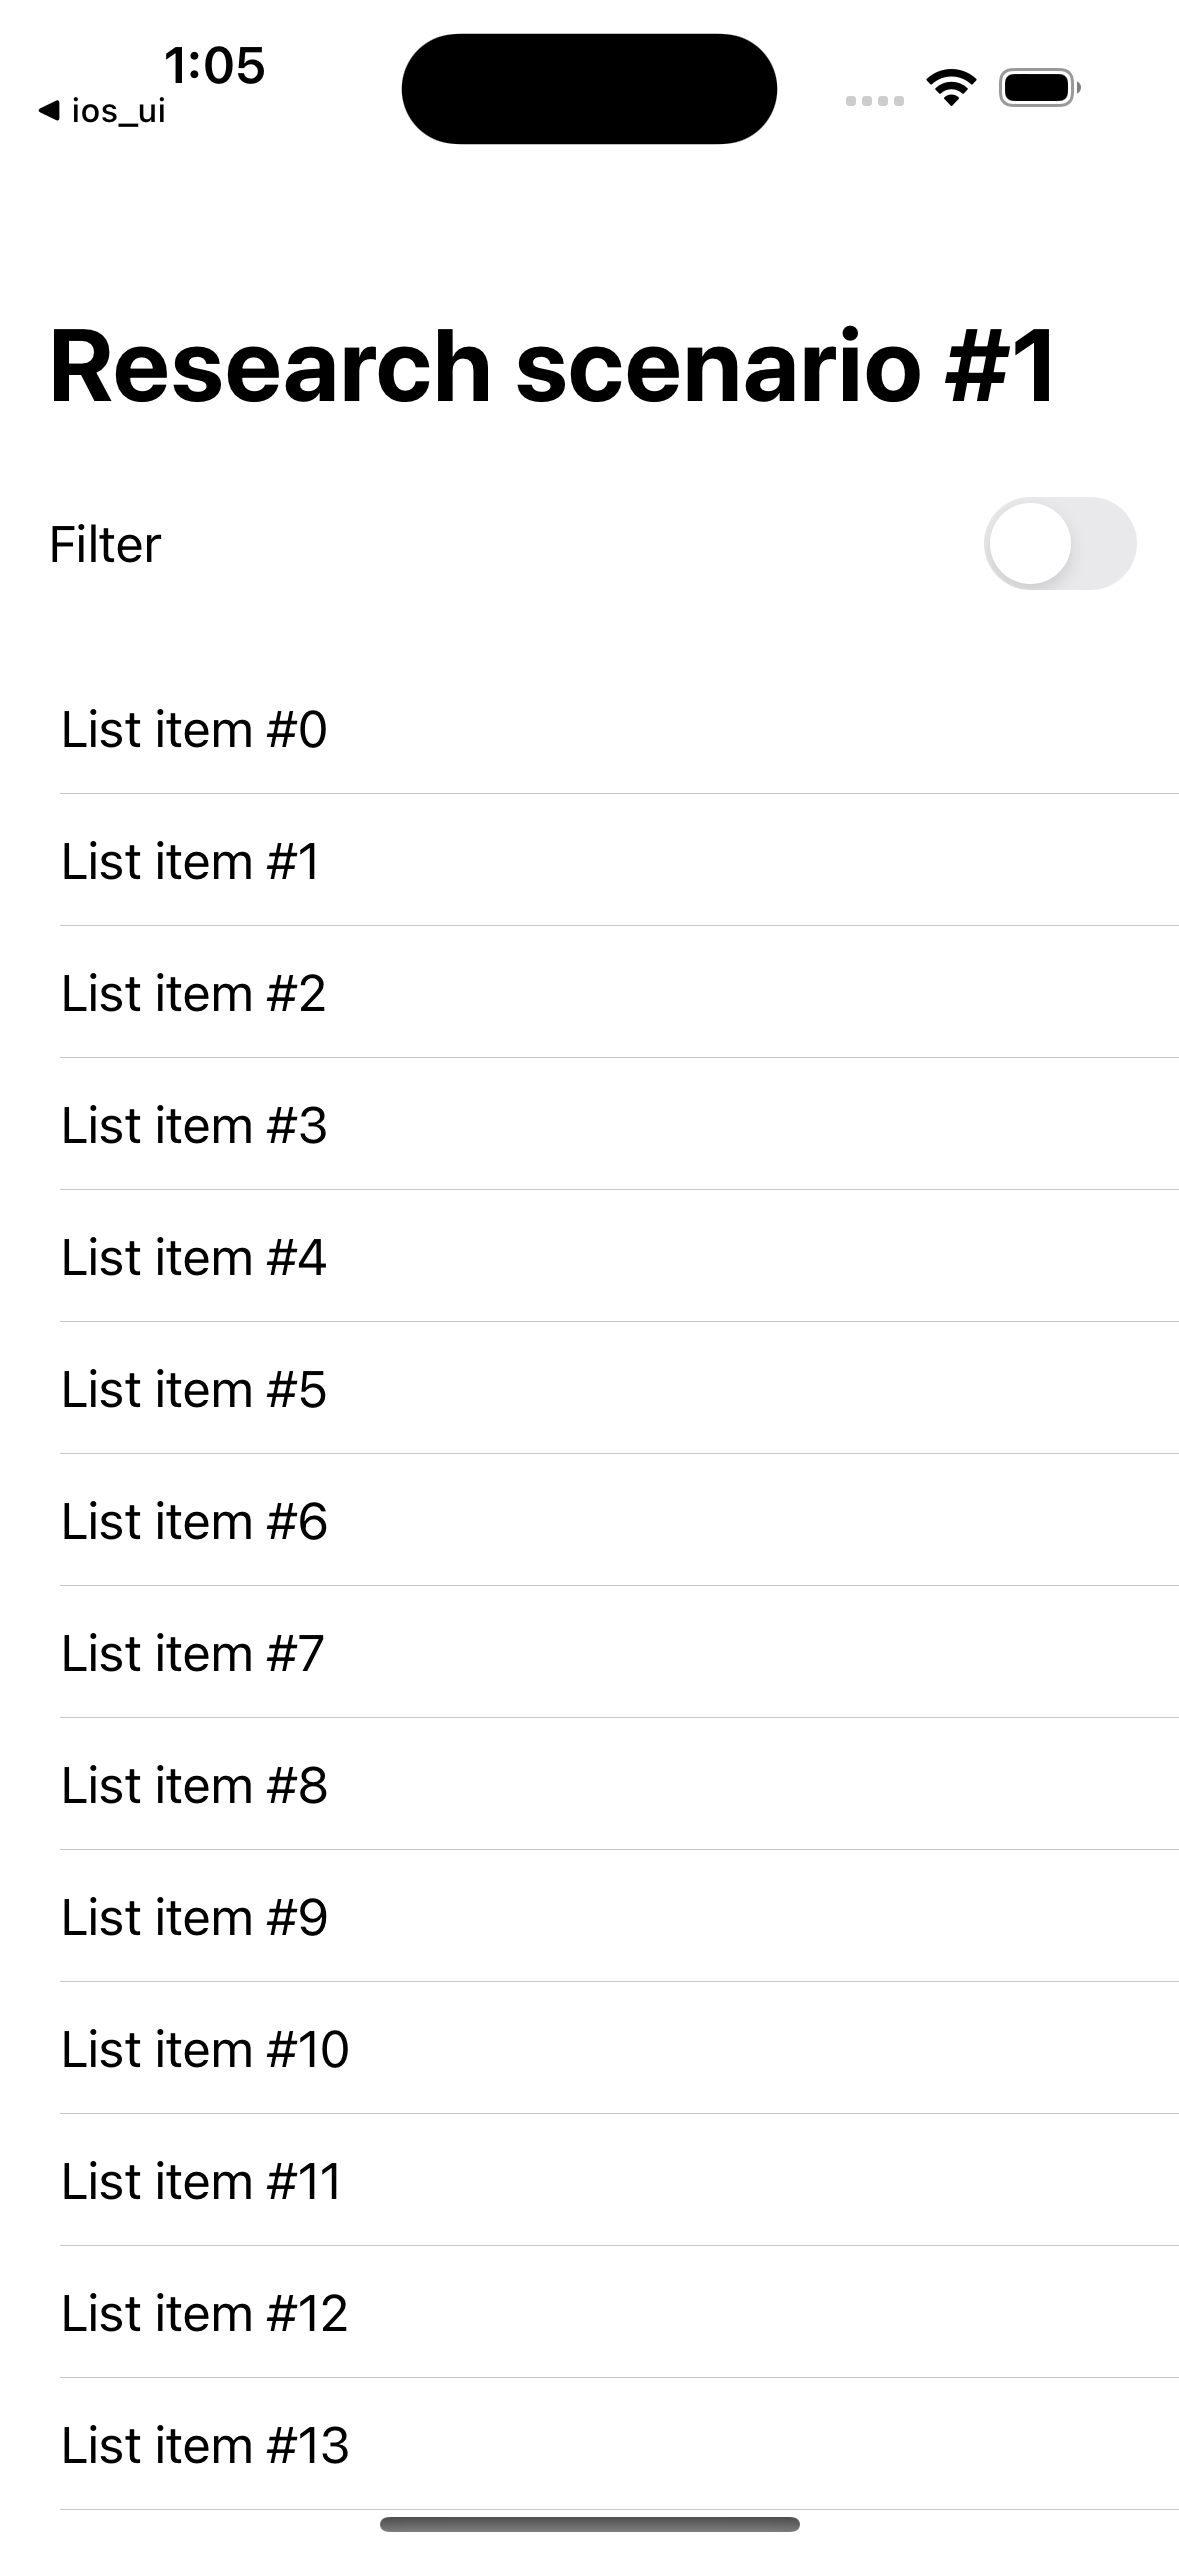
\includegraphics[height=50mm]{img/app1_swift}
      \caption{App 1: Swift (Source: Own work)}
      \label{fig:app1_swift}
    \end{minipage}
\end{figure}

\begin{figure}[H]
  \begin{minipage}{.47\textwidth}
    \centering
    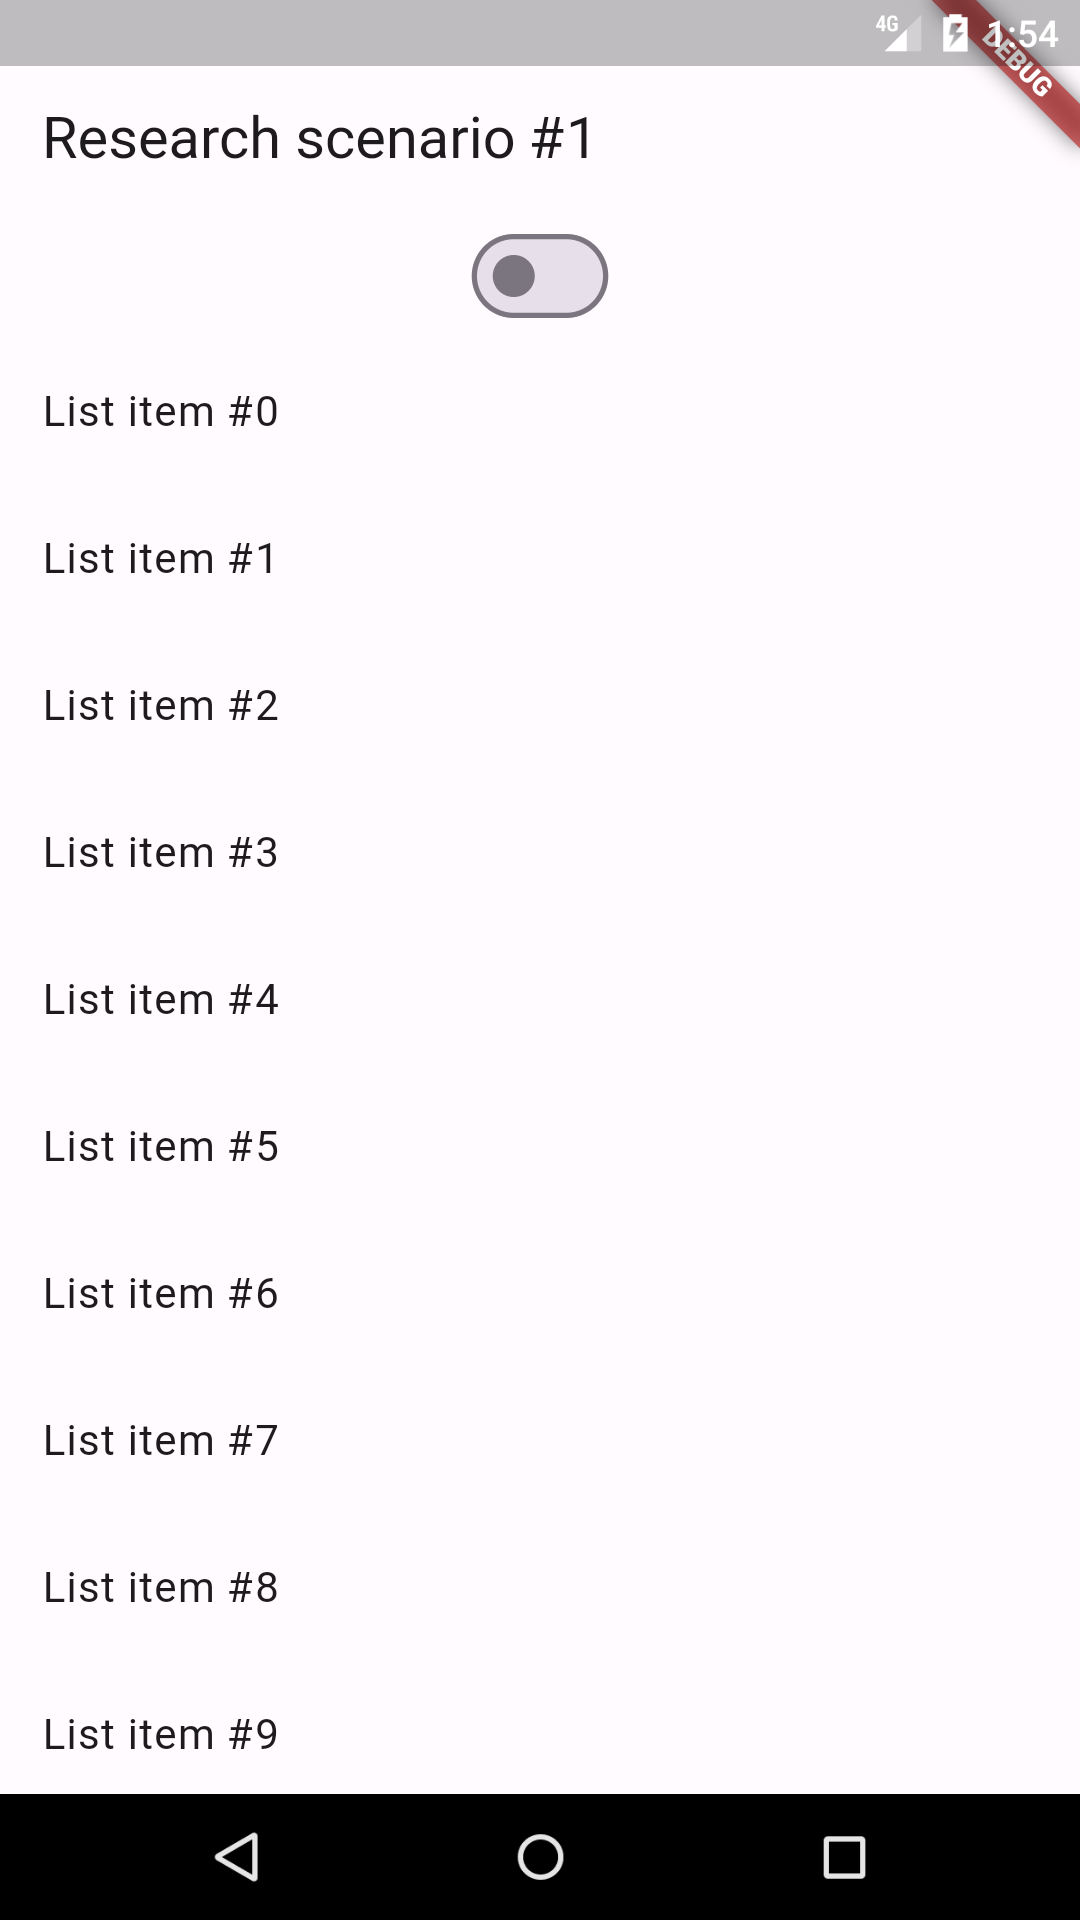
\includegraphics[height=50mm]{img/app1_flutter_android}
    \caption{App 1: Flutter Android (Source: Own work)}
    \label{fig:app1_flutter_android}
  \end{minipage}
  \hfill
  \begin{minipage}{.47\textwidth}
    \centering
    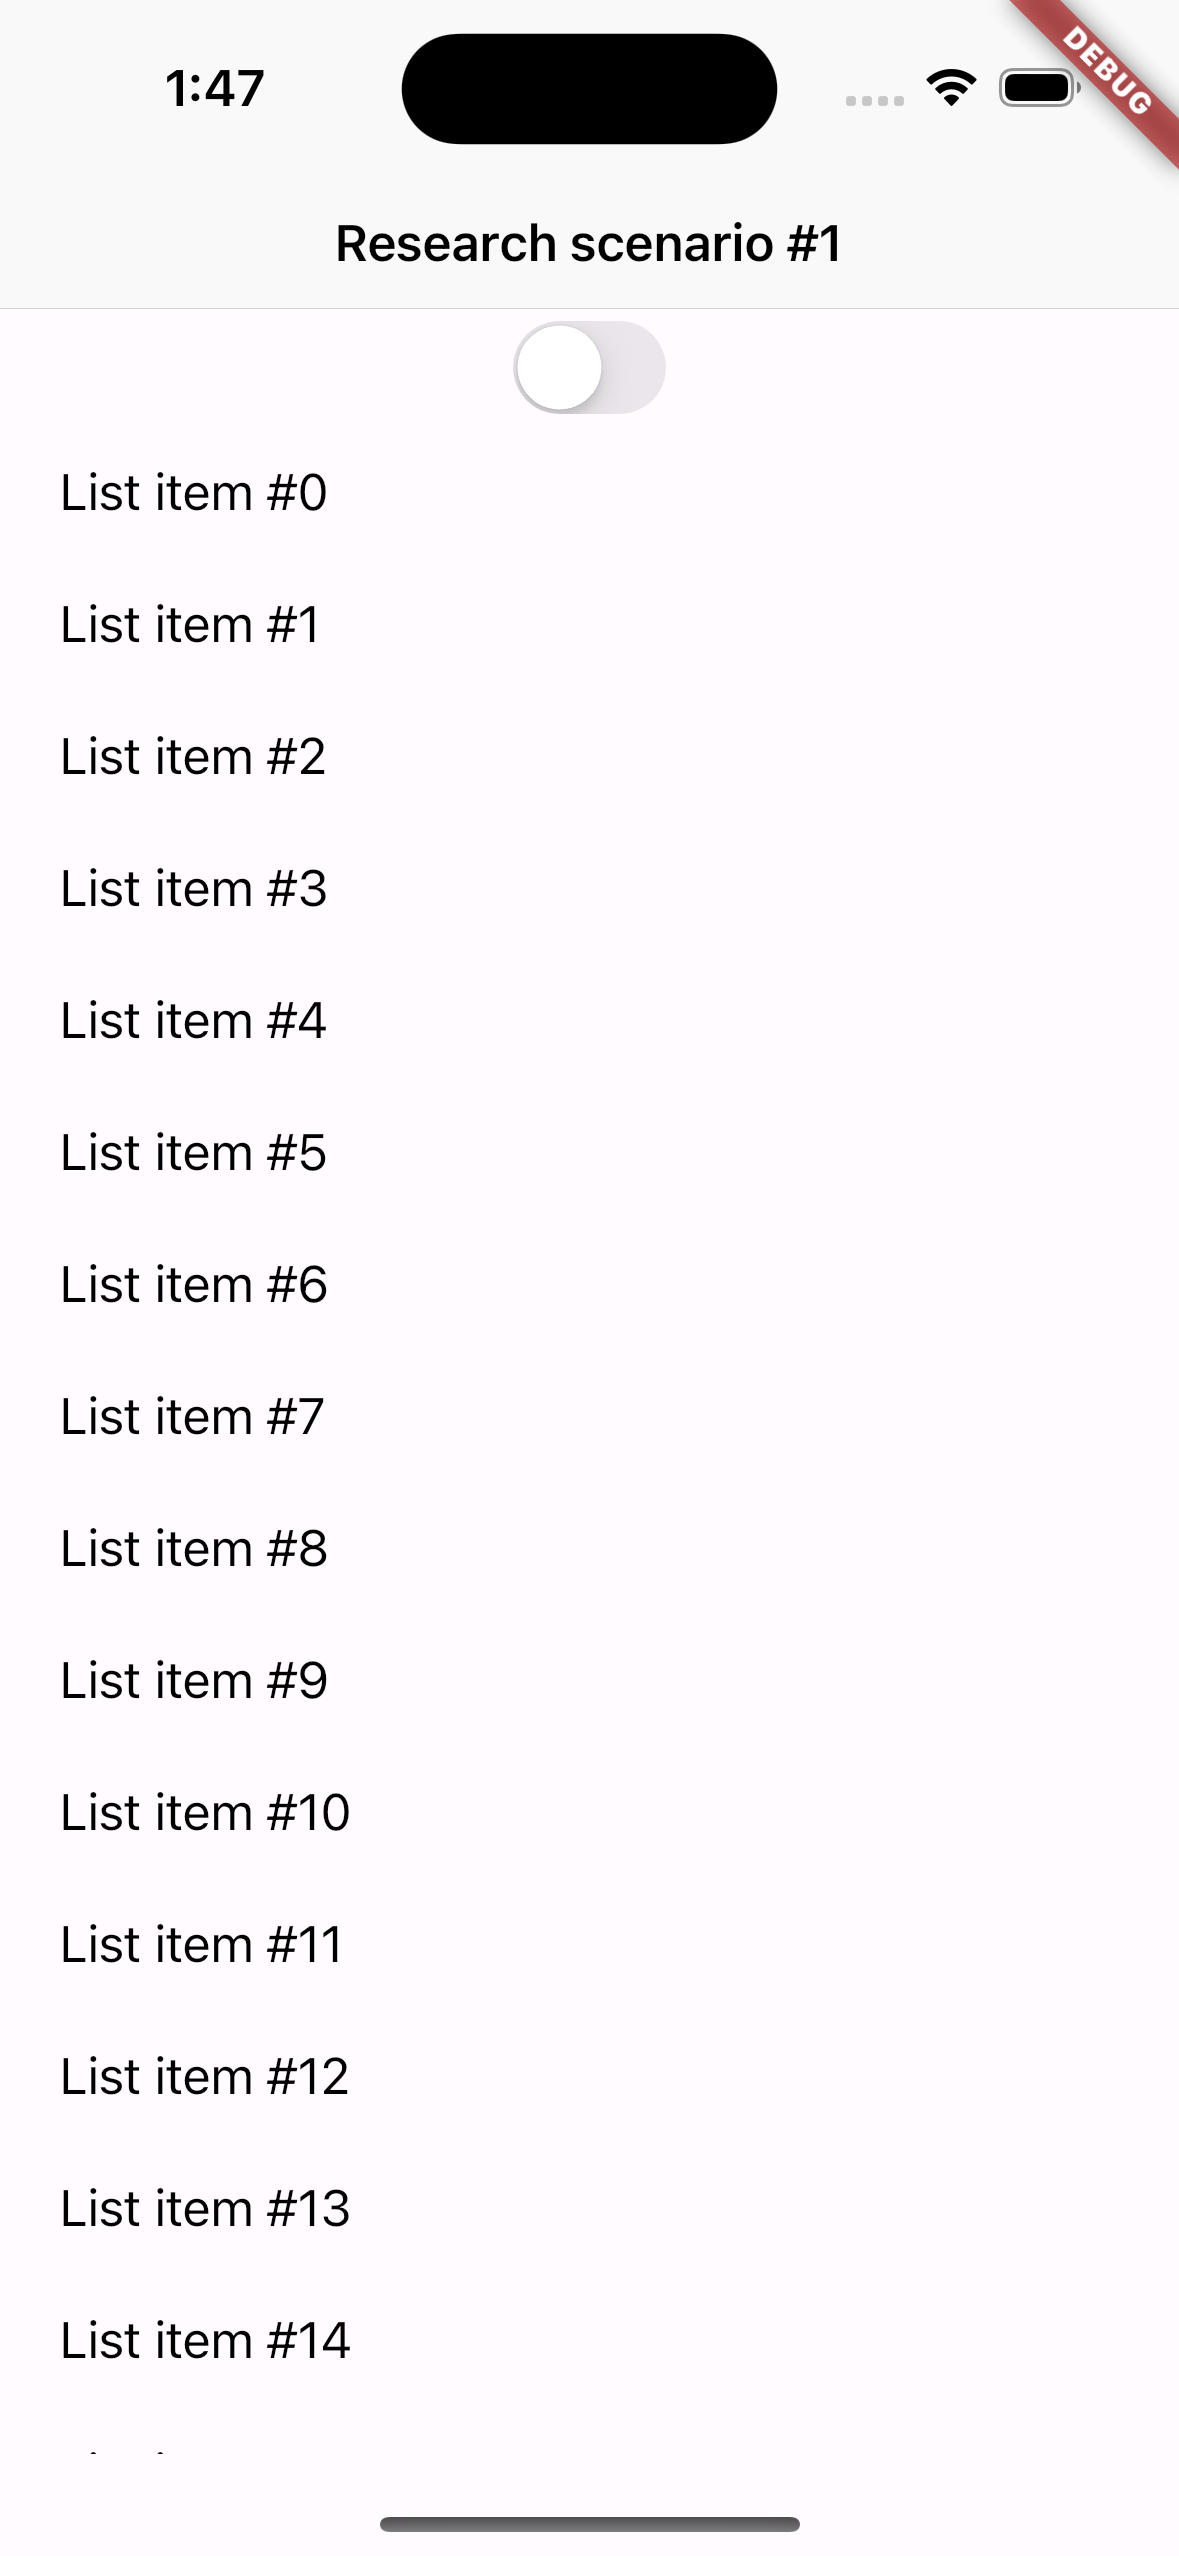
\includegraphics[height=50mm]{img/app1_flutter_ios}
    \caption{App 1: Flutter iOS (Source: Own work)}
    \label{fig:app1_flutter_ios}
  \end{minipage}
\end{figure}

\begin{figure}[H]
  \begin{minipage}{.47\textwidth}
    \centering
    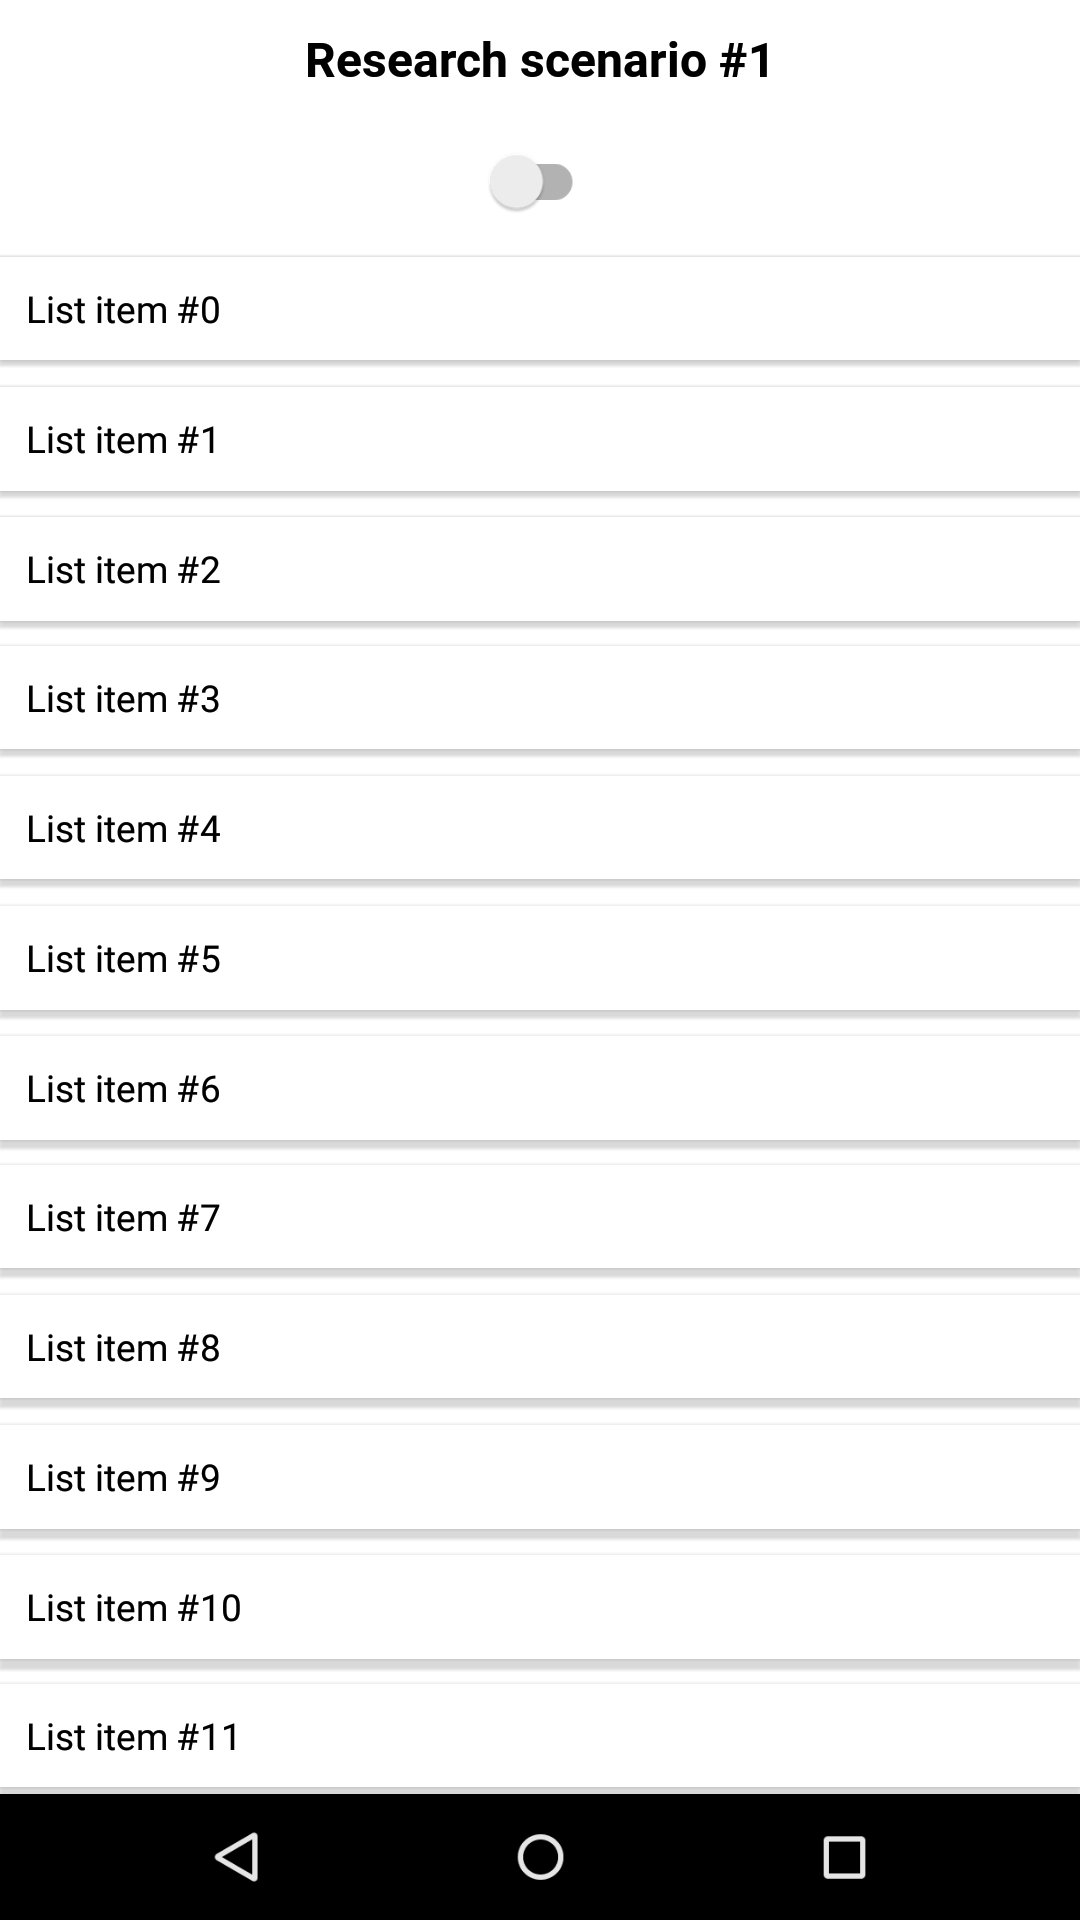
\includegraphics[height=50mm]{img/app1_rn_android}
    \caption{App 1: React Native Android (Source: Own work)}
    \label{fig:app1_rn_android}
  \end{minipage}
  \hfill
  \begin{minipage}{.47\textwidth}
    \centering
    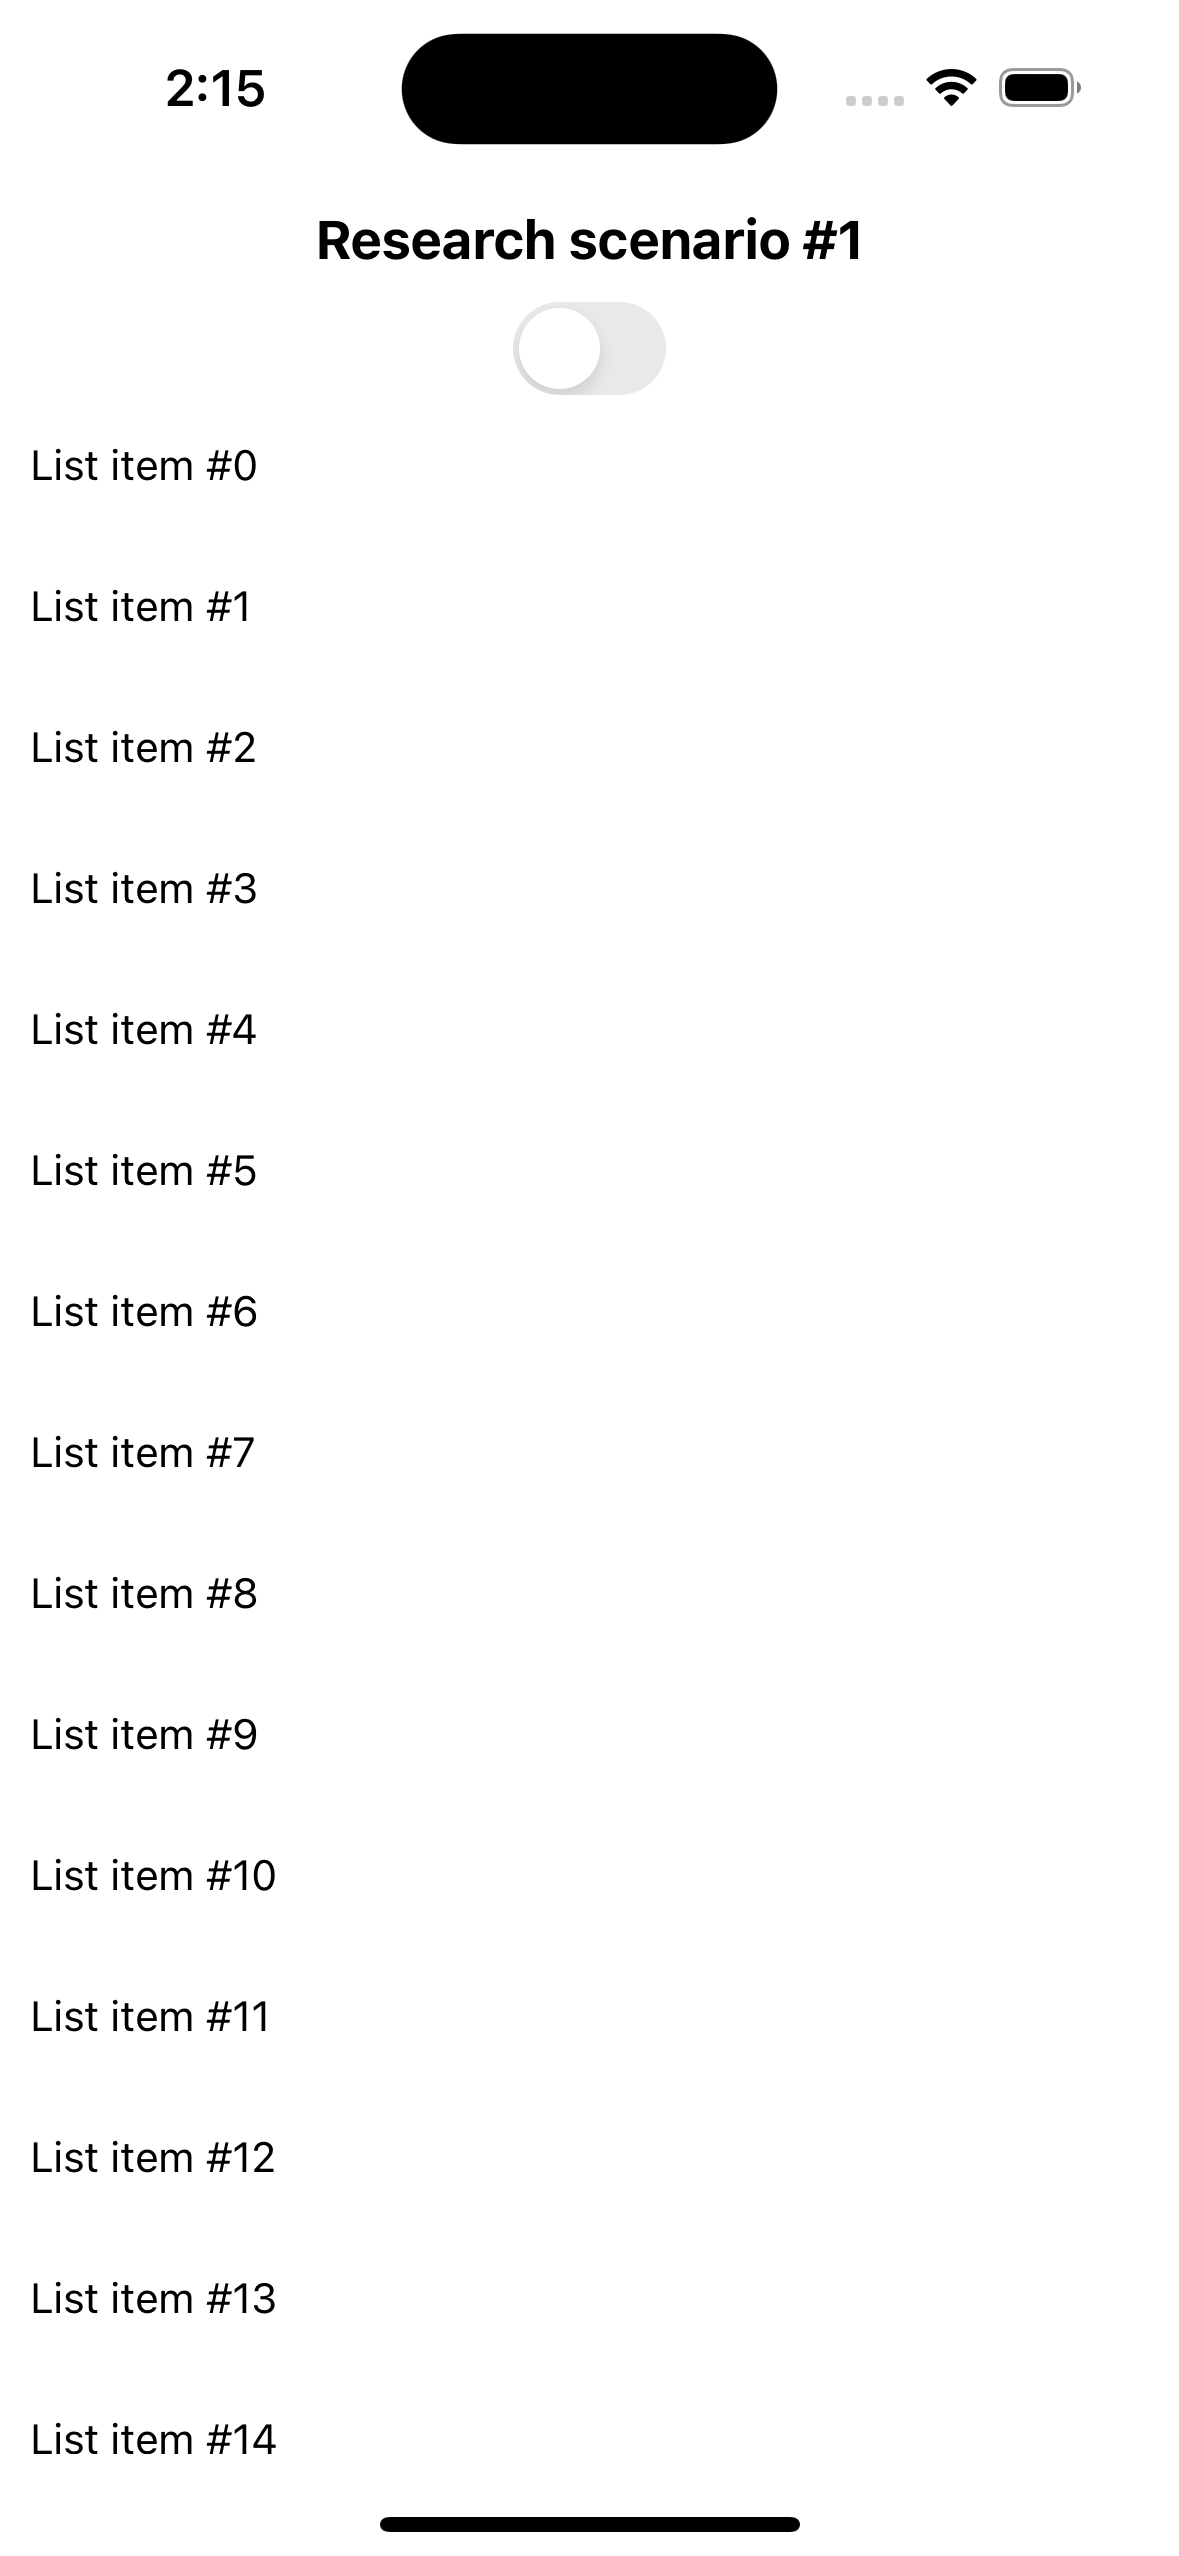
\includegraphics[height=50mm]{img/app1_rn_ios}
    \caption{App 1: React Native iOS (Source: Own work)}
    \label{fig:app1_rn_ios}
  \end{minipage}
\end{figure}

\section{Research scenario 2: Animations}

The application consists of rows of \emph{RotatingIcons} and \emph{GrowingIcons}. The former animates its rotation and the latter animates its size, with different durations and directions.

\begin{figure}[H]
  \begin{minipage}{.47\textwidth}
    \centering
    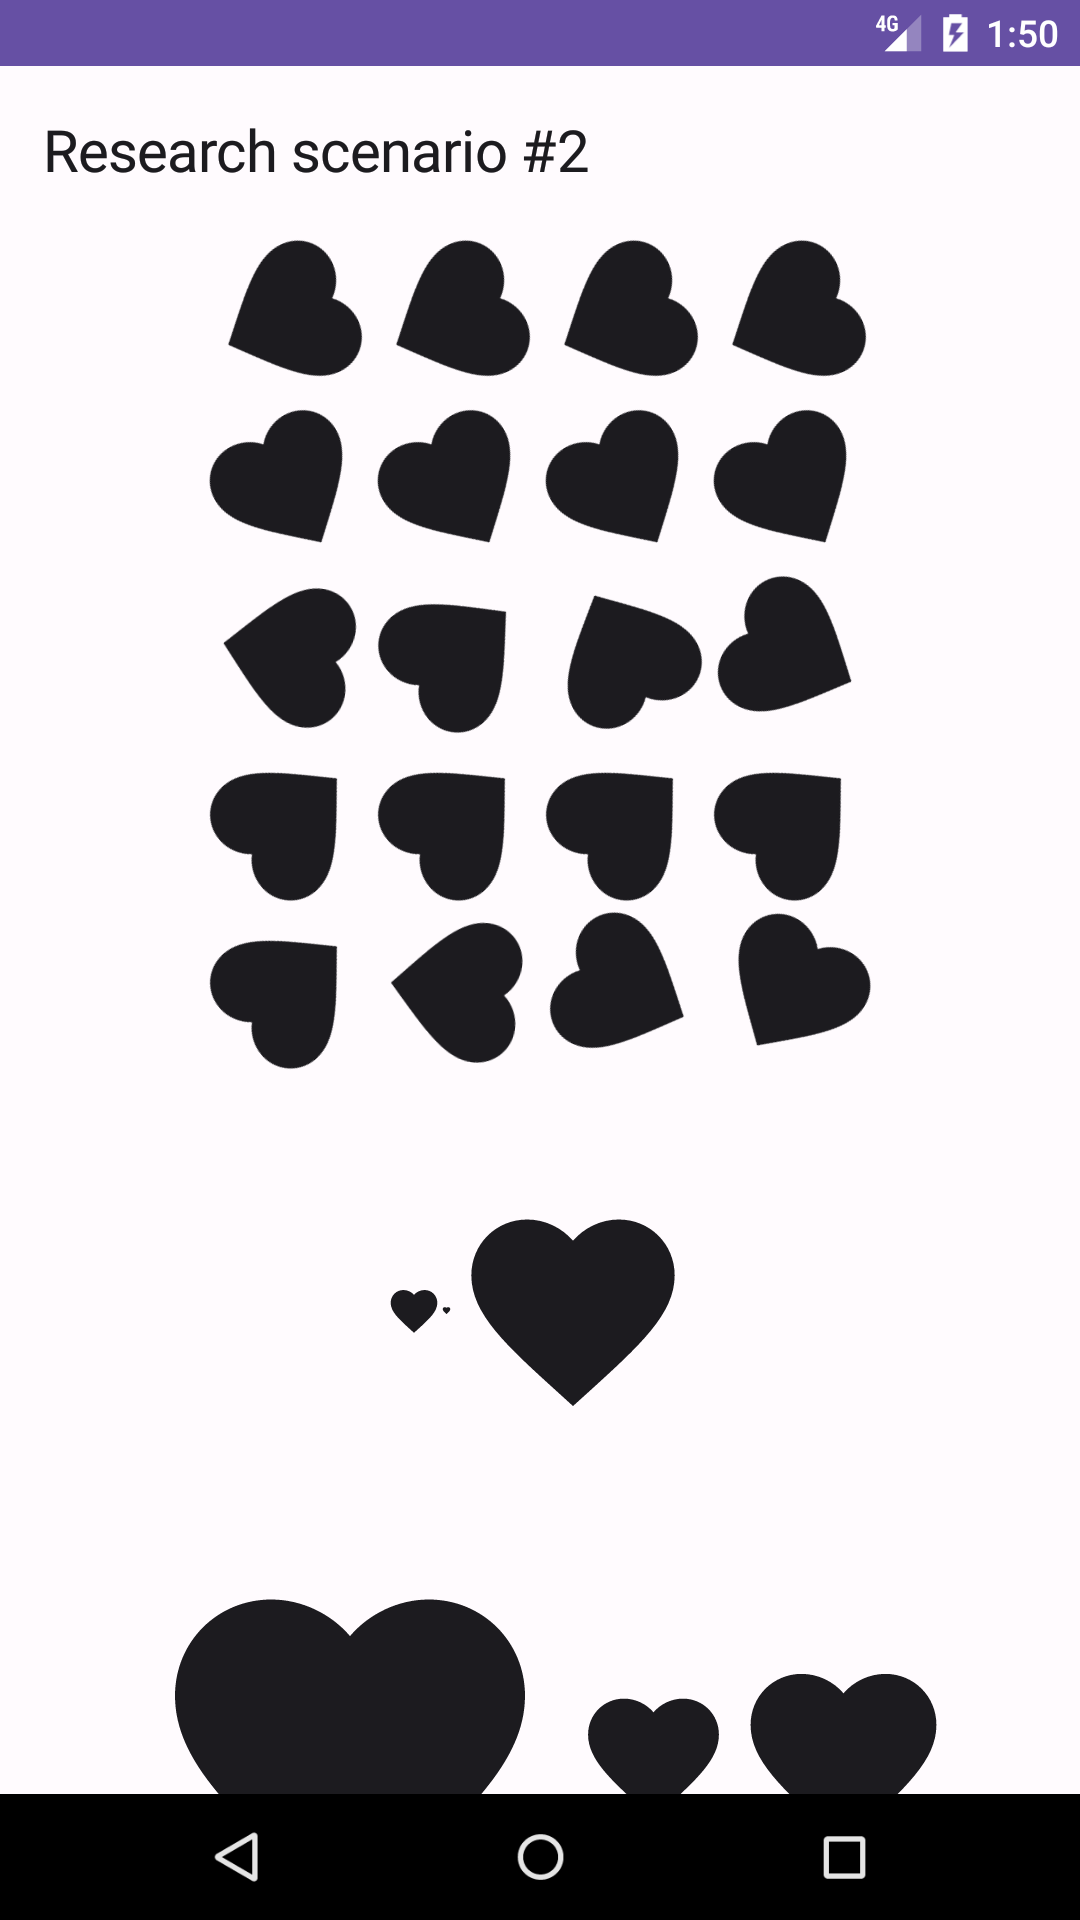
\includegraphics[height=50mm]{img/app2_kotlin}
    \caption{App 2: Kotlin (Source: Own work)}
    \label{fig:app2_kotlin}
  \end{minipage}
  \hfill
  \begin{minipage}{.47\textwidth}
    \centering
    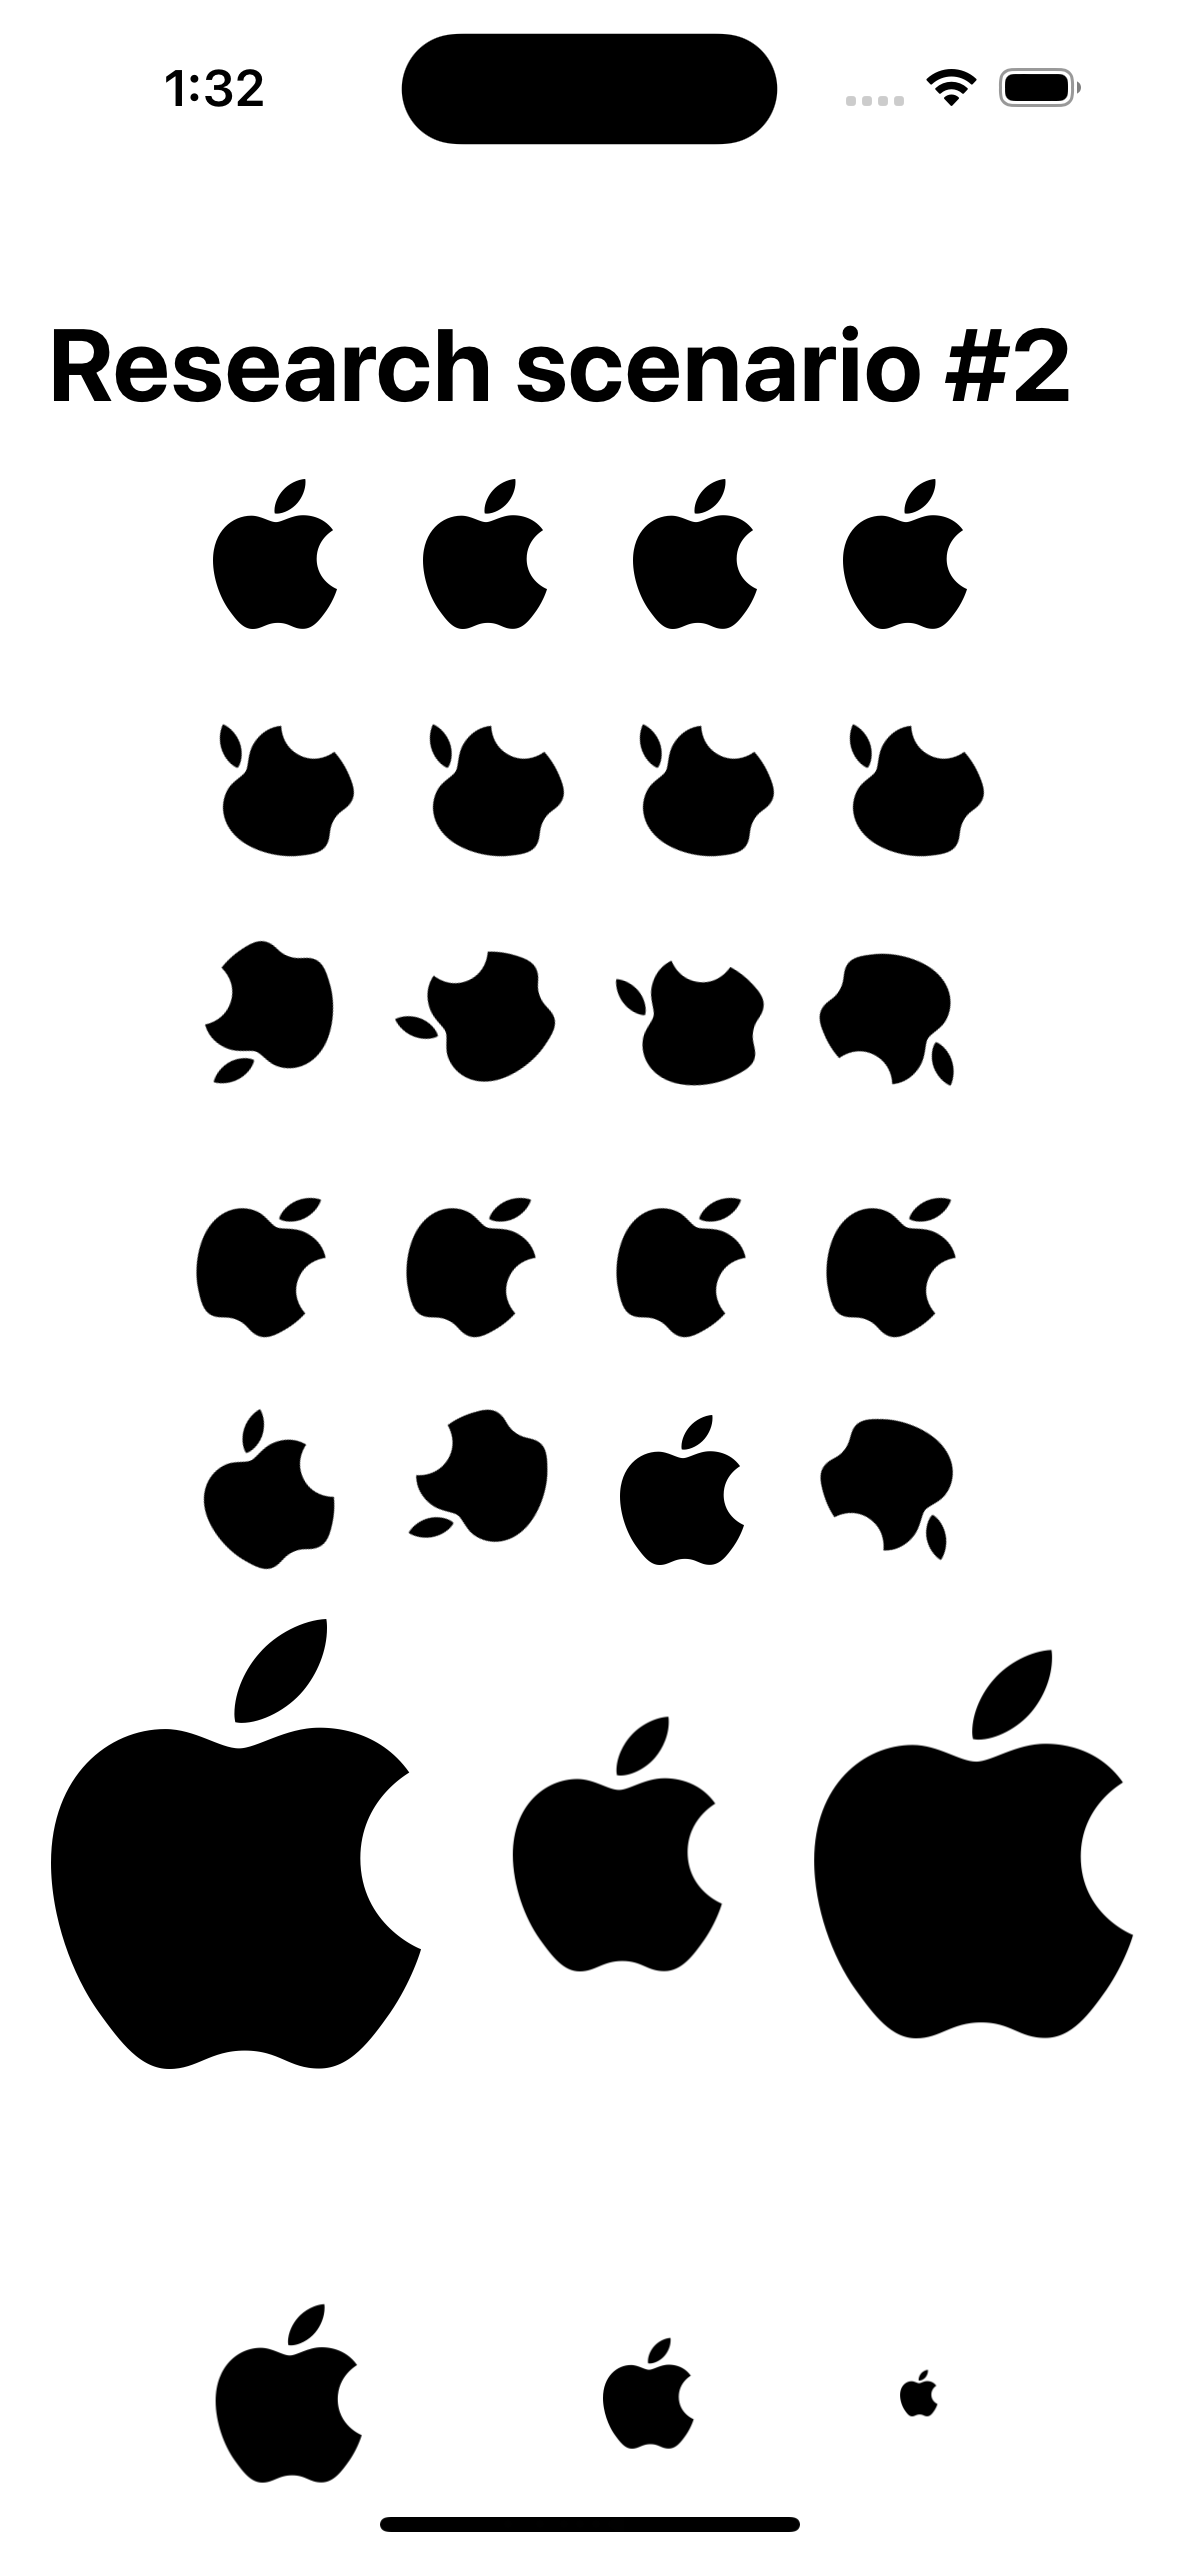
\includegraphics[height=50mm]{img/app2_swift}
    \caption{App 2: Swift (Source: Own work)}
    \label{fig:app2_swift}
  \end{minipage}
\end{figure}

\begin{figure}[H]
\begin{minipage}{.47\textwidth}
  \centering
  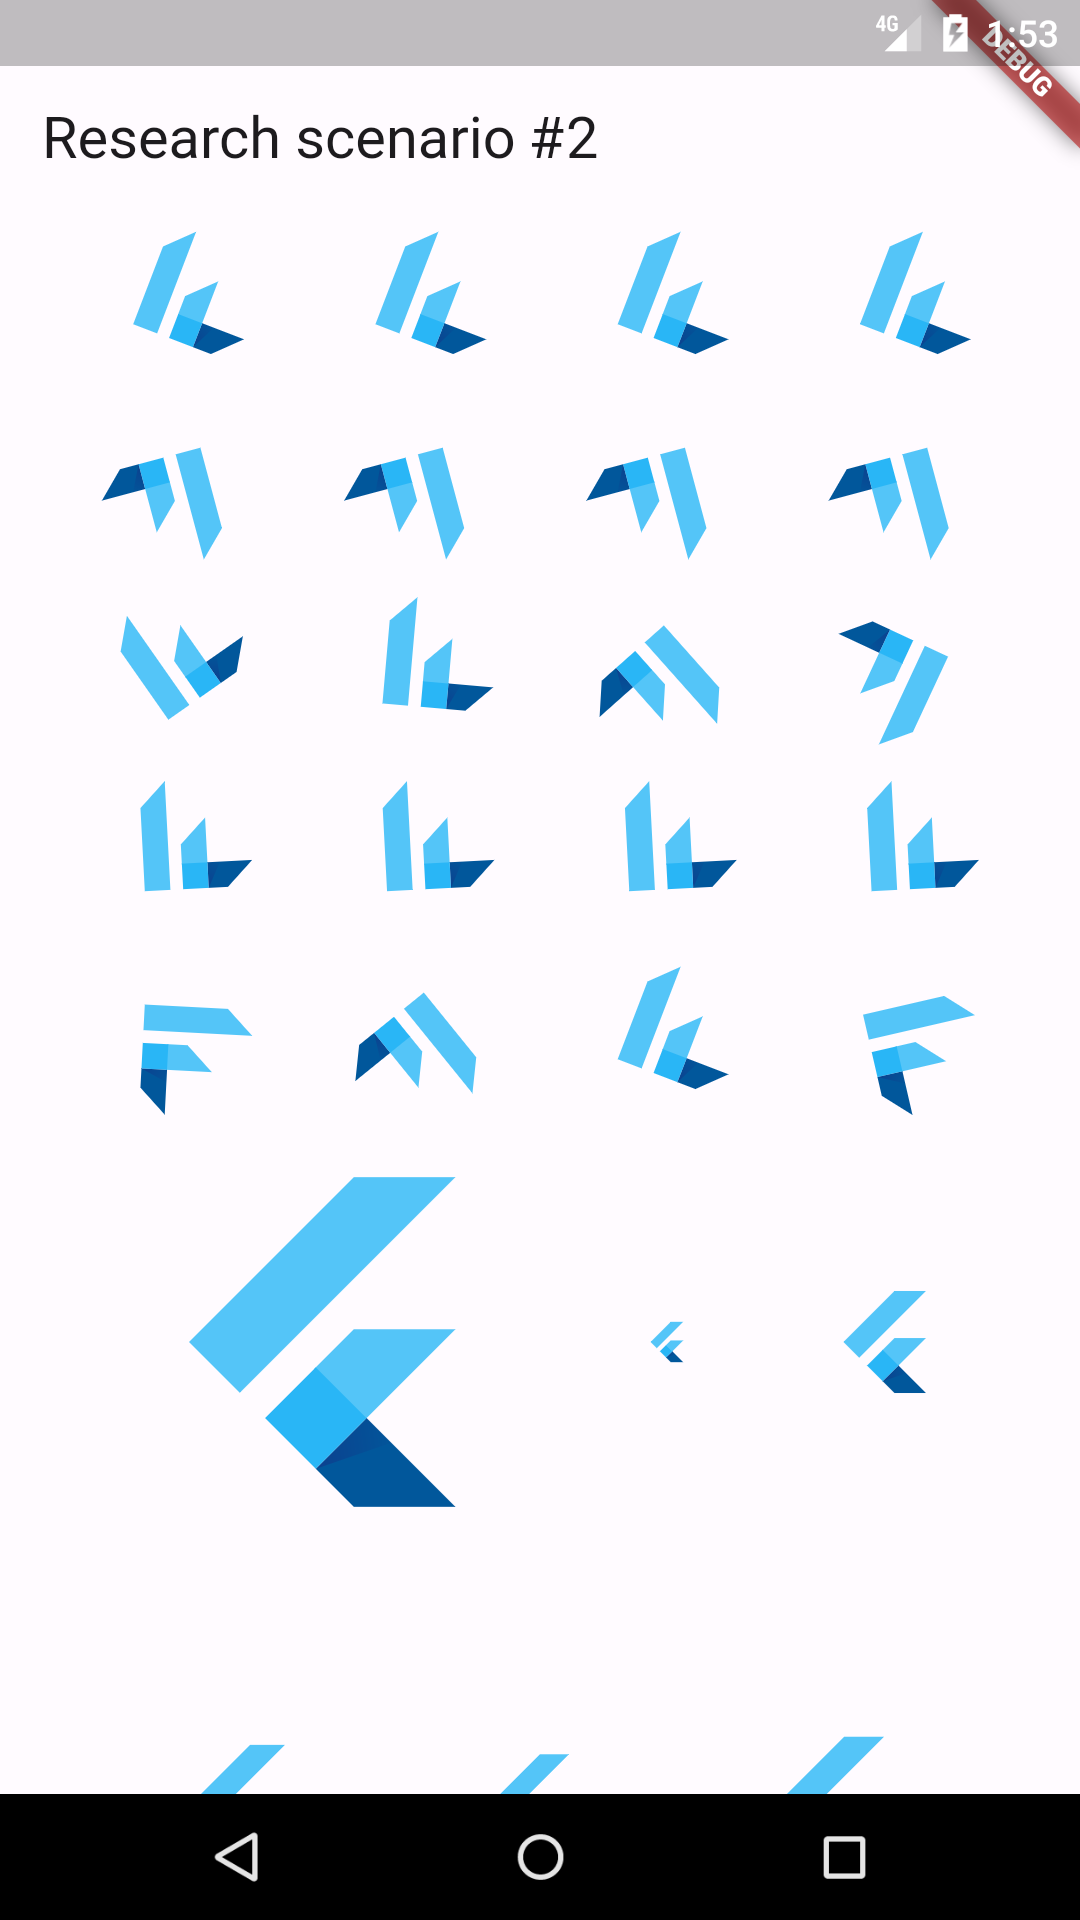
\includegraphics[height=50mm]{img/app2_flutter_android}
  \caption{App 2: Flutter Android (Source: Own work)}
  \label{fig:app2_flutter_android}
\end{minipage}
\hfill
\begin{minipage}{.47\textwidth}
  \centering
  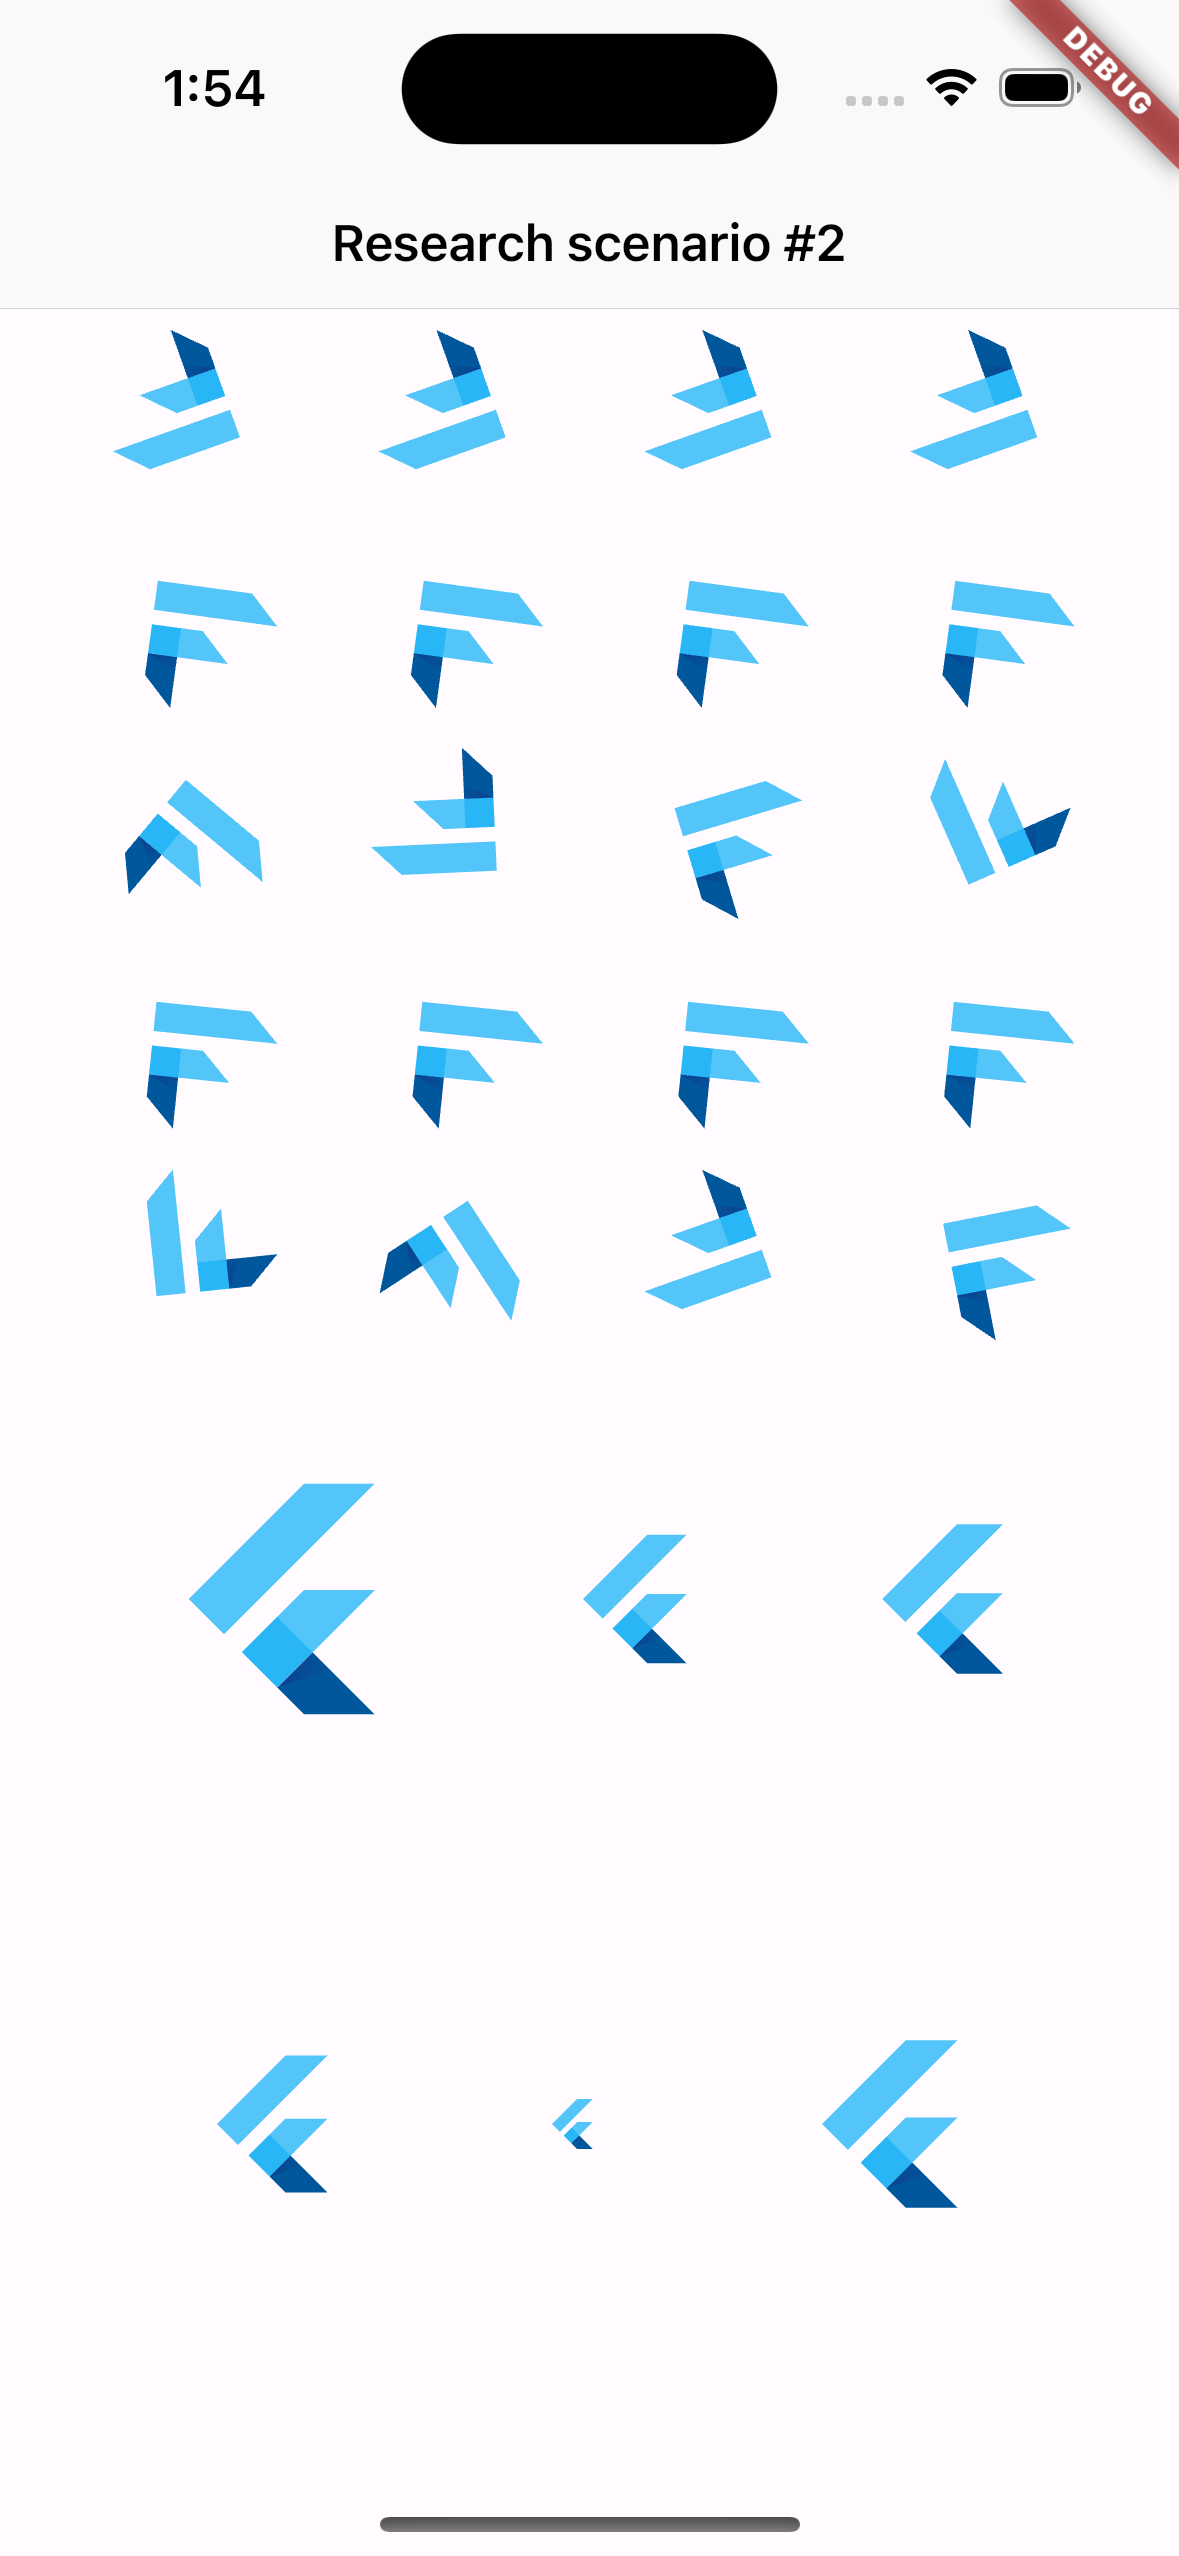
\includegraphics[height=50mm]{img/app2_flutter_ios}
  \caption{App 2: Flutter iOS (Source: Own work)}
  \label{fig:app2_flutter_ios}
\end{minipage}
\end{figure}

\begin{figure}[H]
\begin{minipage}{.47\textwidth}
  \centering
  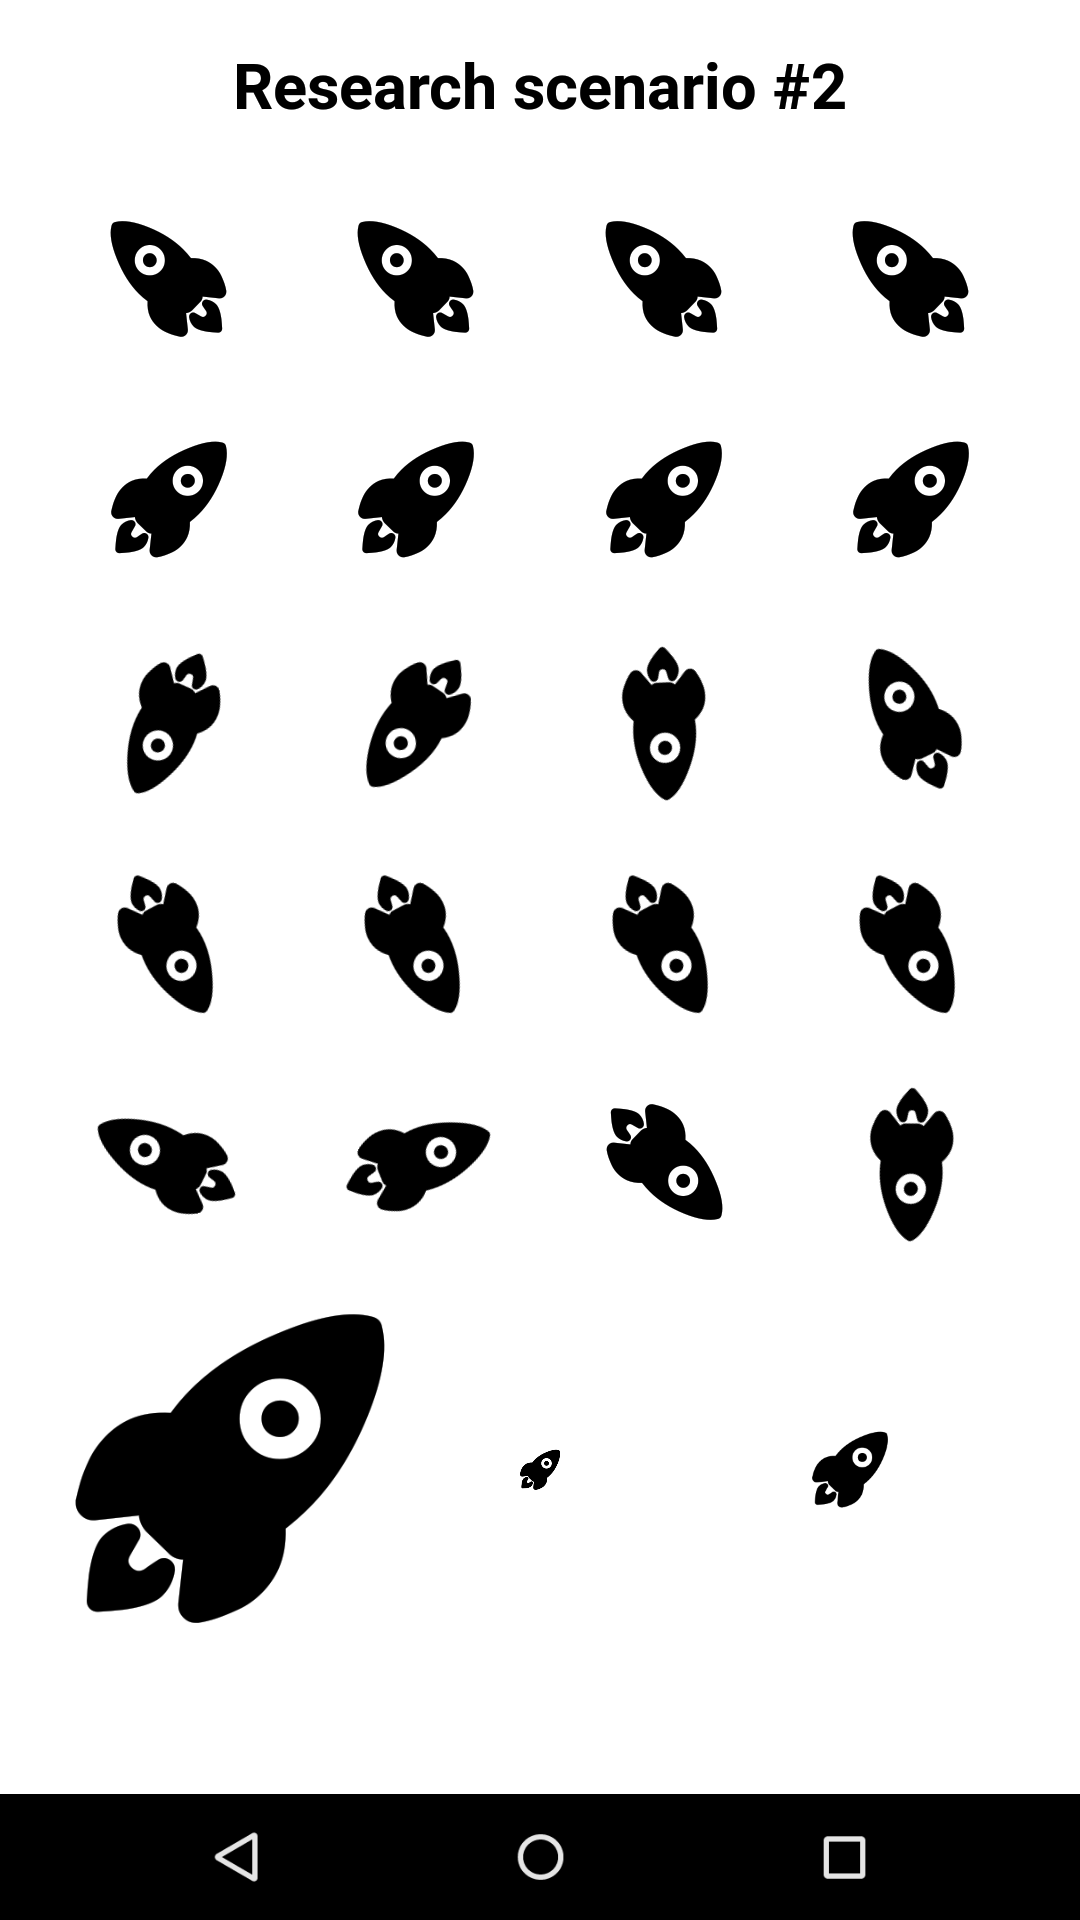
\includegraphics[height=50mm]{img/app2_rn_android}
  \caption{App 1: React Native Android (Source: Own work)}
  \label{fig:app2_rn_android}
\end{minipage}
\hfill
\begin{minipage}{.47\textwidth}
  \centering
  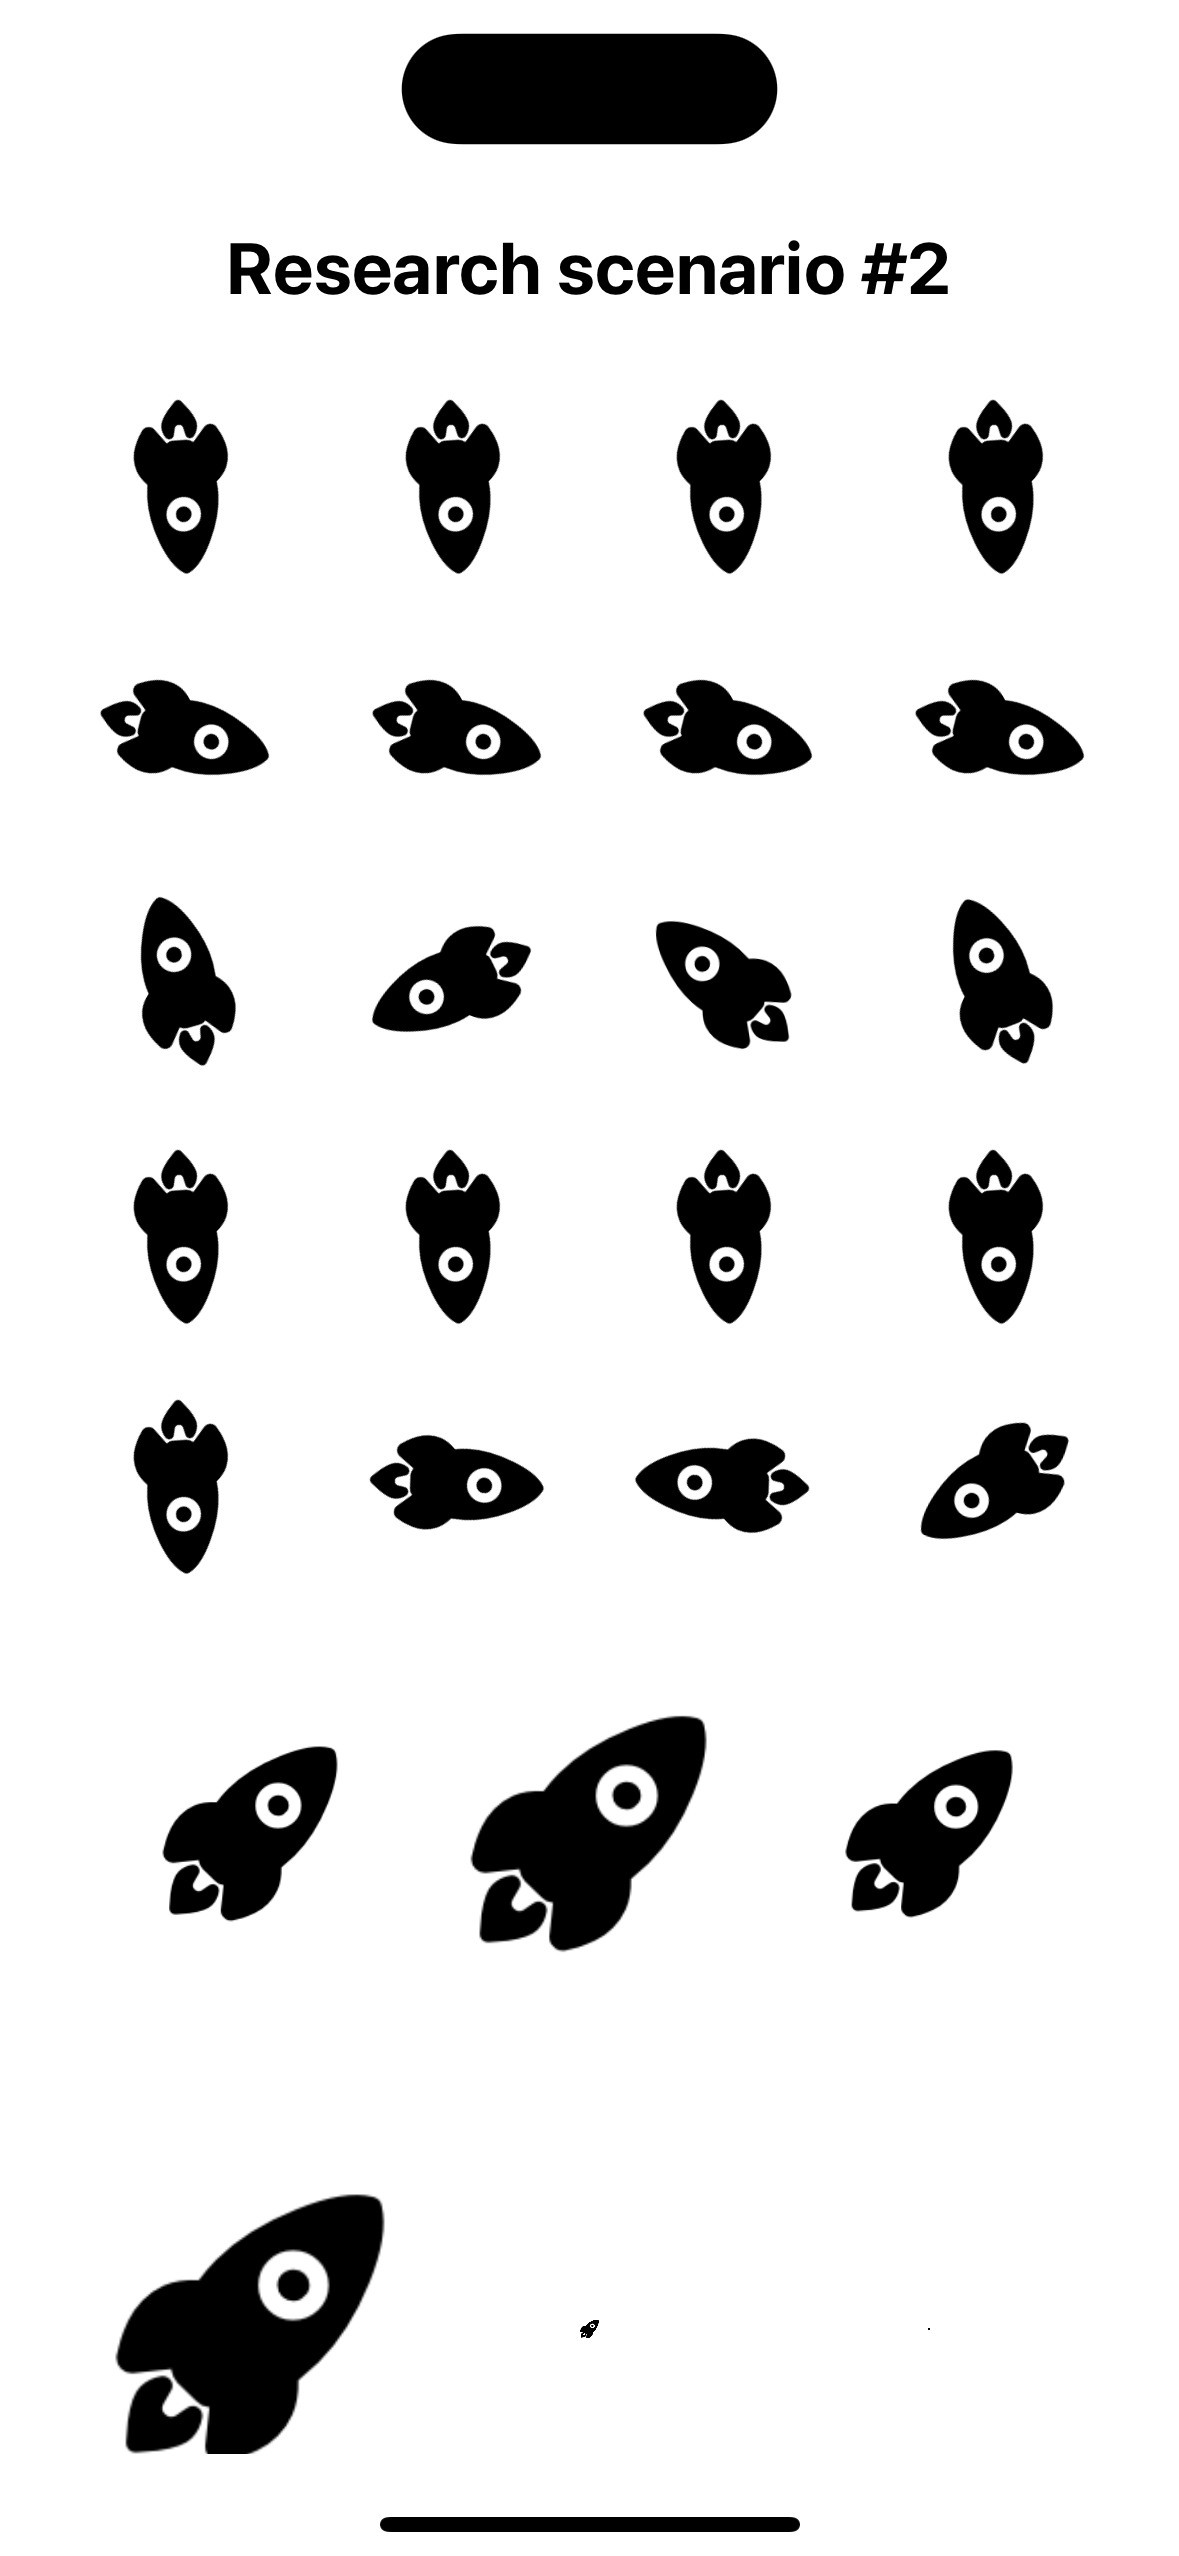
\includegraphics[height=50mm]{img/app2_rn_ios}
  \caption{App 1: React Native iOS (Source: Own work)}
  \label{fig:app2_rn_ios}
\end{minipage}
\end{figure}

\section{Research scenario 3: File I/O}

The application consists of two \emph{Buttons} and a \emph{Grid View}. The first \emph{Button} saves a text file on the device and the second allows selecting images from the Gallery. Selected images are then presented in a 2-column scrollable \emph{Grid view}.

\begin{figure}[H]
  \begin{minipage}{.47\textwidth}
    \centering
    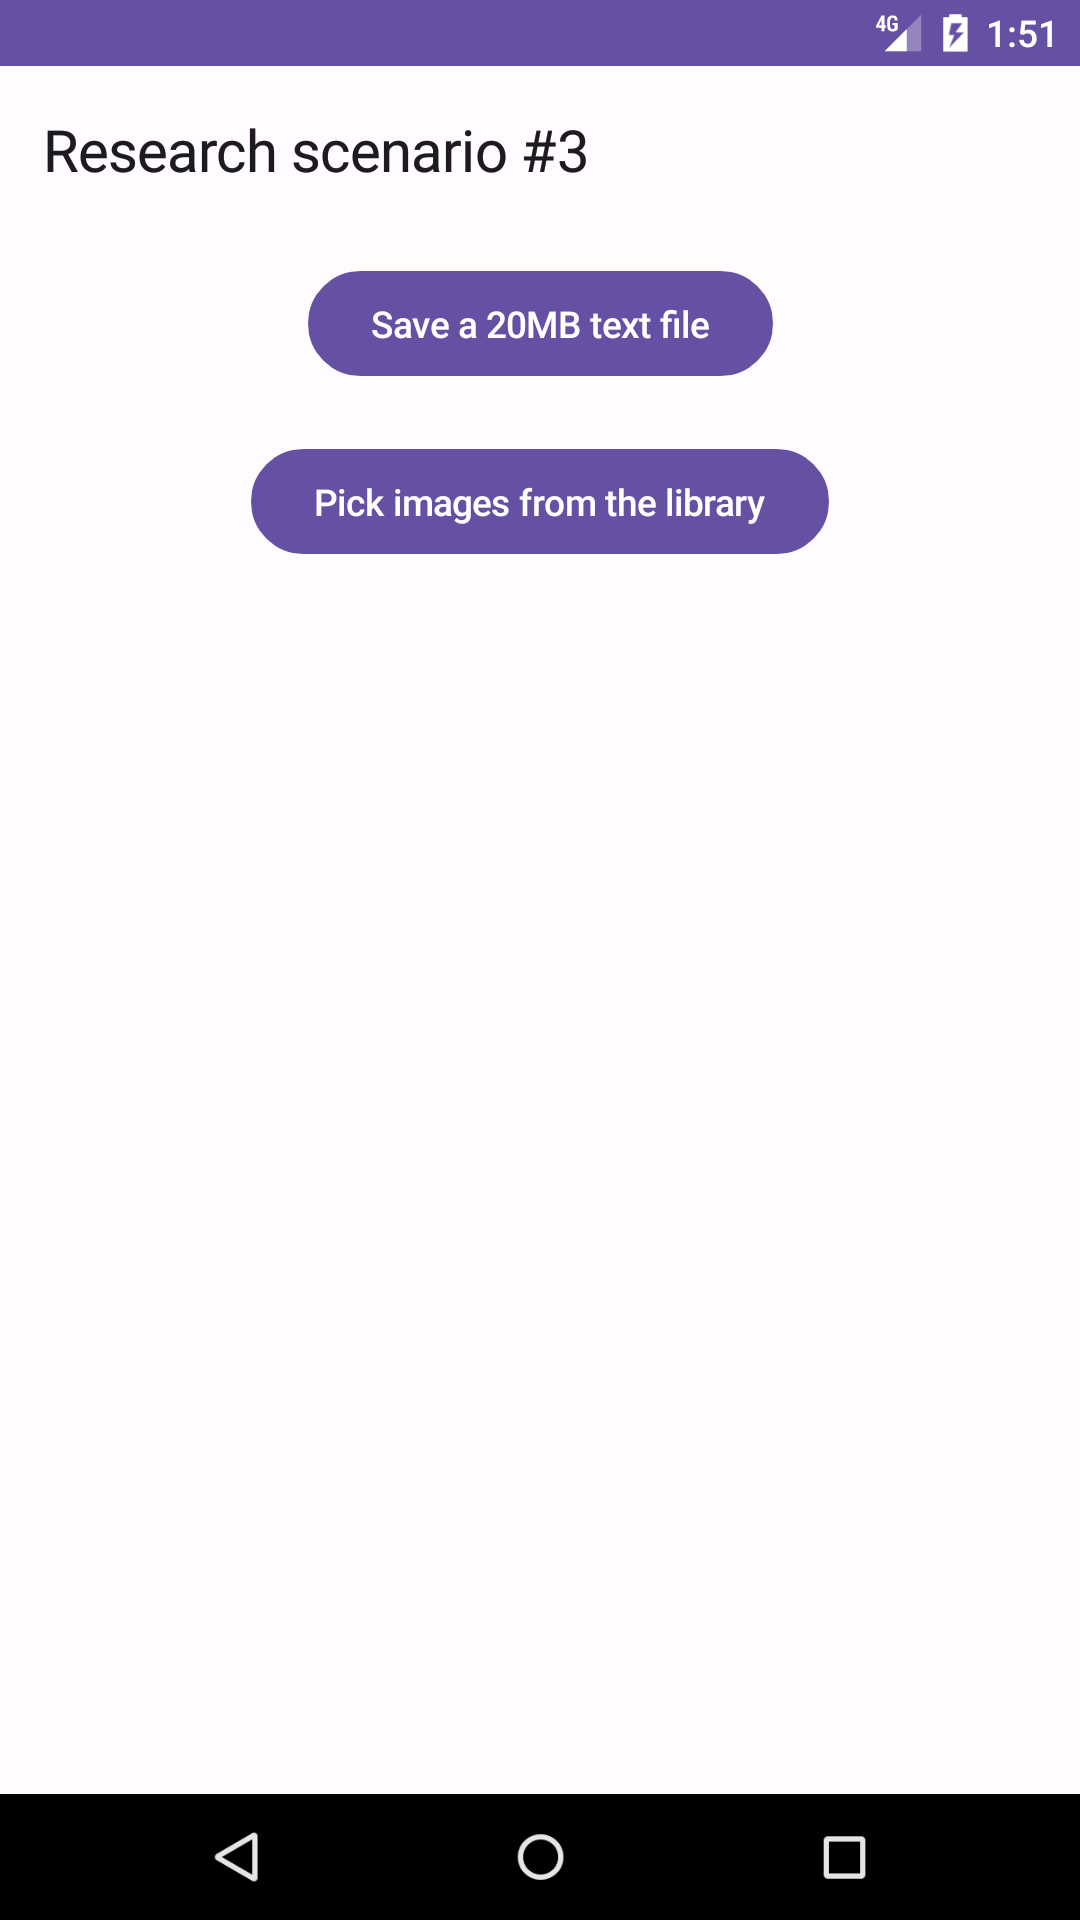
\includegraphics[height=50mm]{img/app3_kotlin}
    \caption{App 3: Kotlin (Source: Own work)}
    \label{fig:app3_kotlin}
  \end{minipage}
  \hfill
  \begin{minipage}{.47\textwidth}
    \centering
    \frame{
      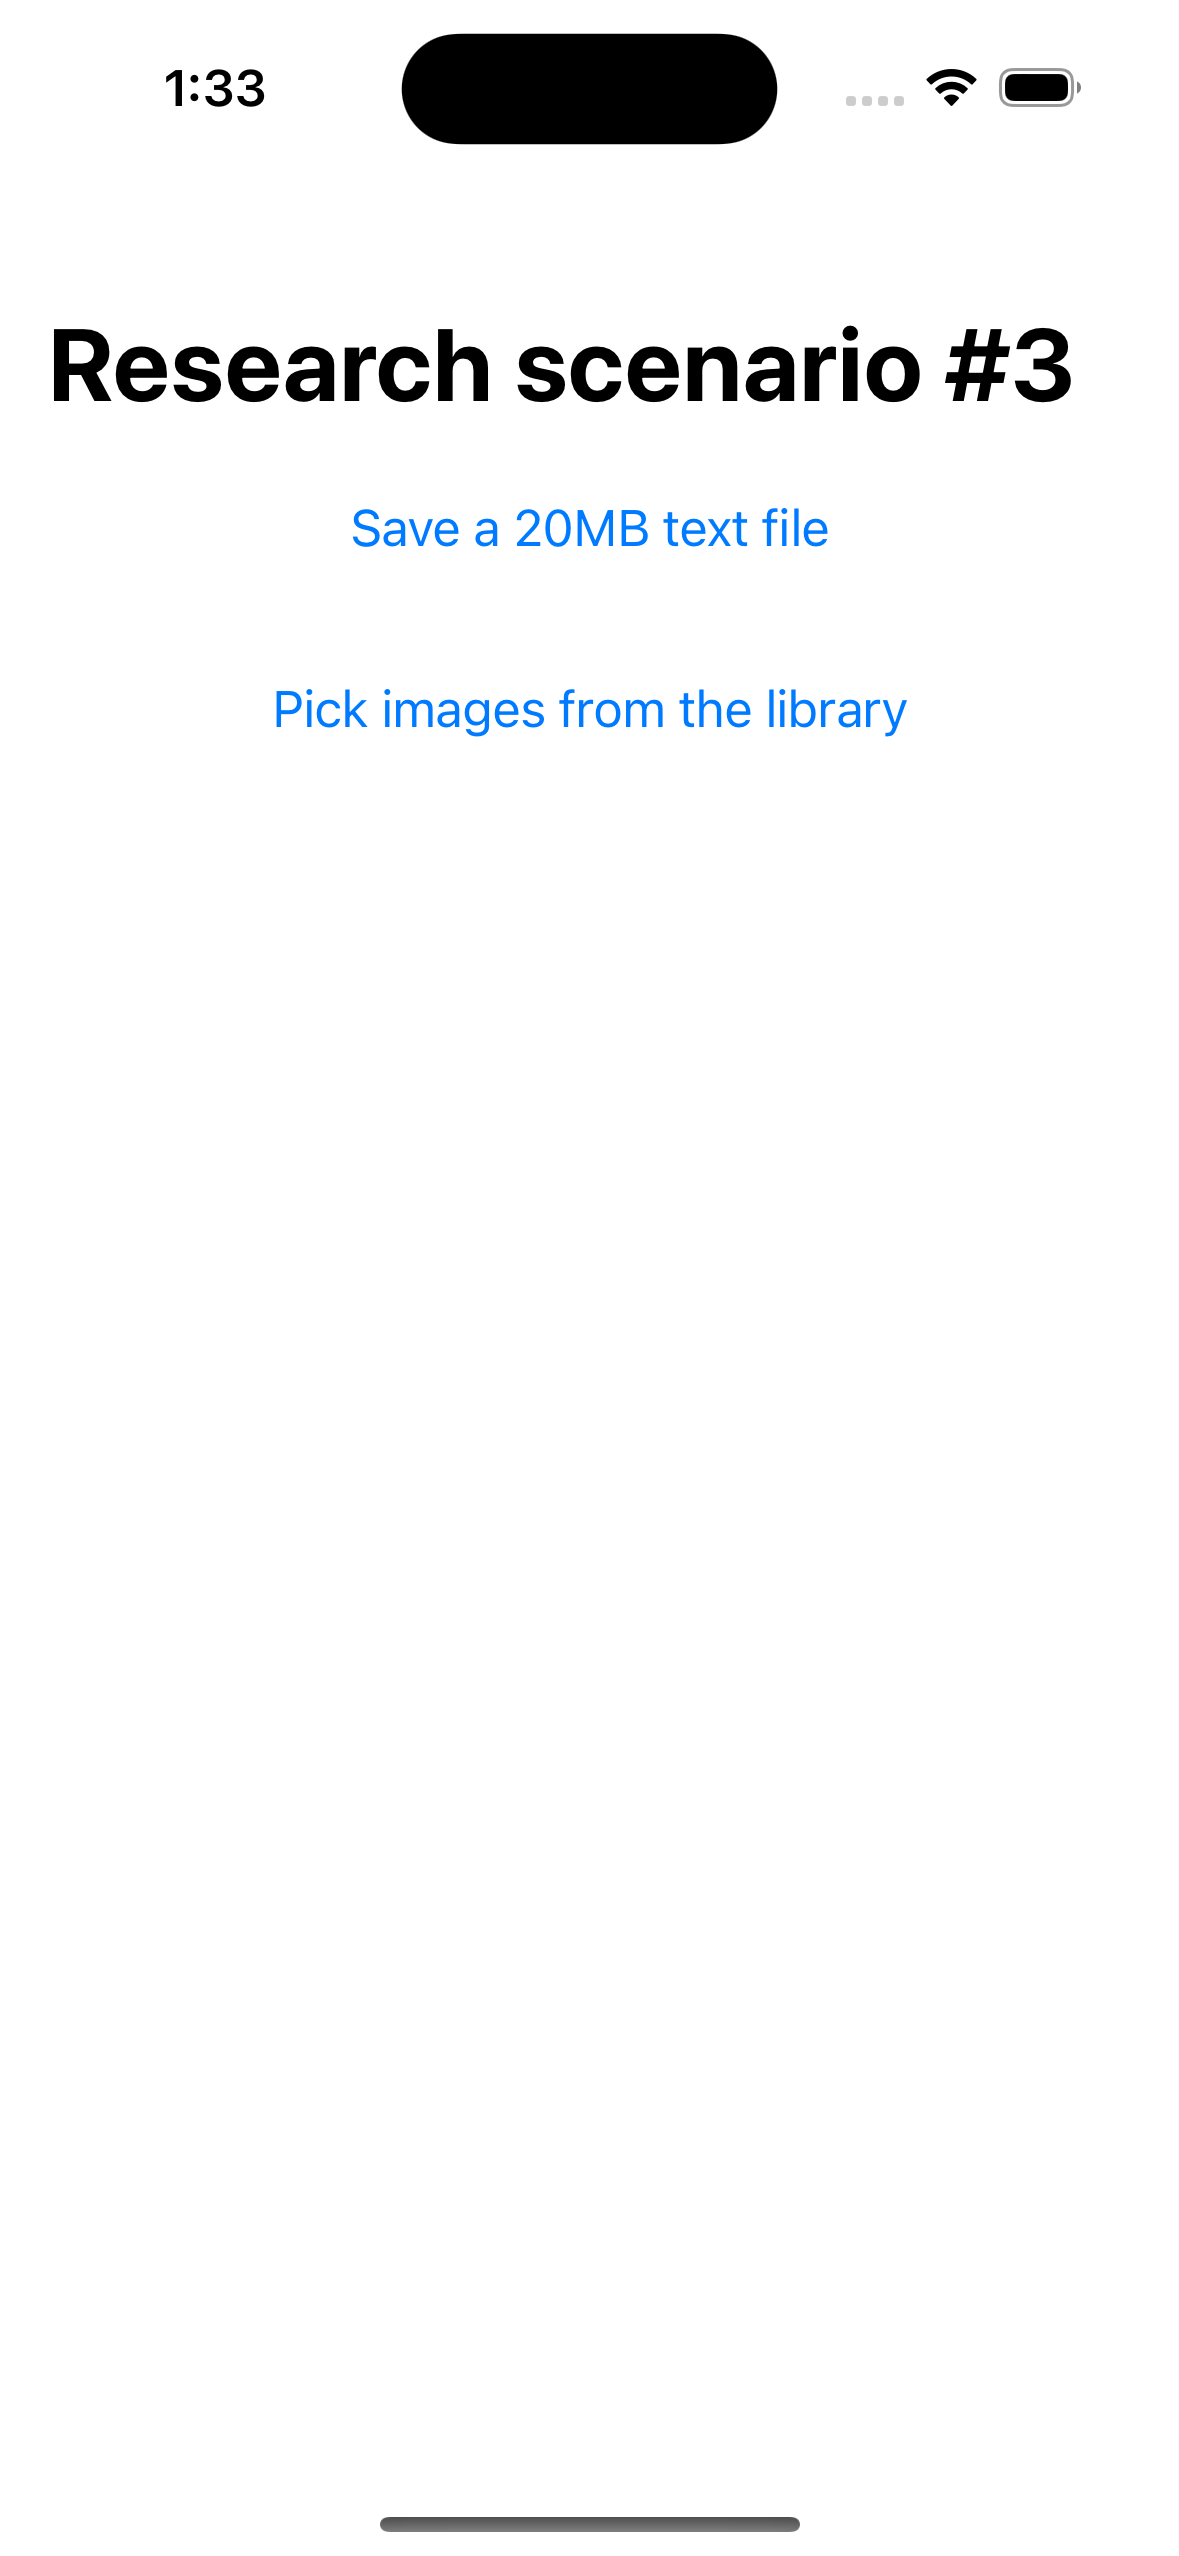
\includegraphics[height=50mm]{img/app3_swift}
    }
    \caption{App 3: Swift (Source: Own work)}
    \label{fig:app3_swift}
  \end{minipage}
\end{figure}

\begin{figure}[H]
\begin{minipage}{.47\textwidth}
  \centering
  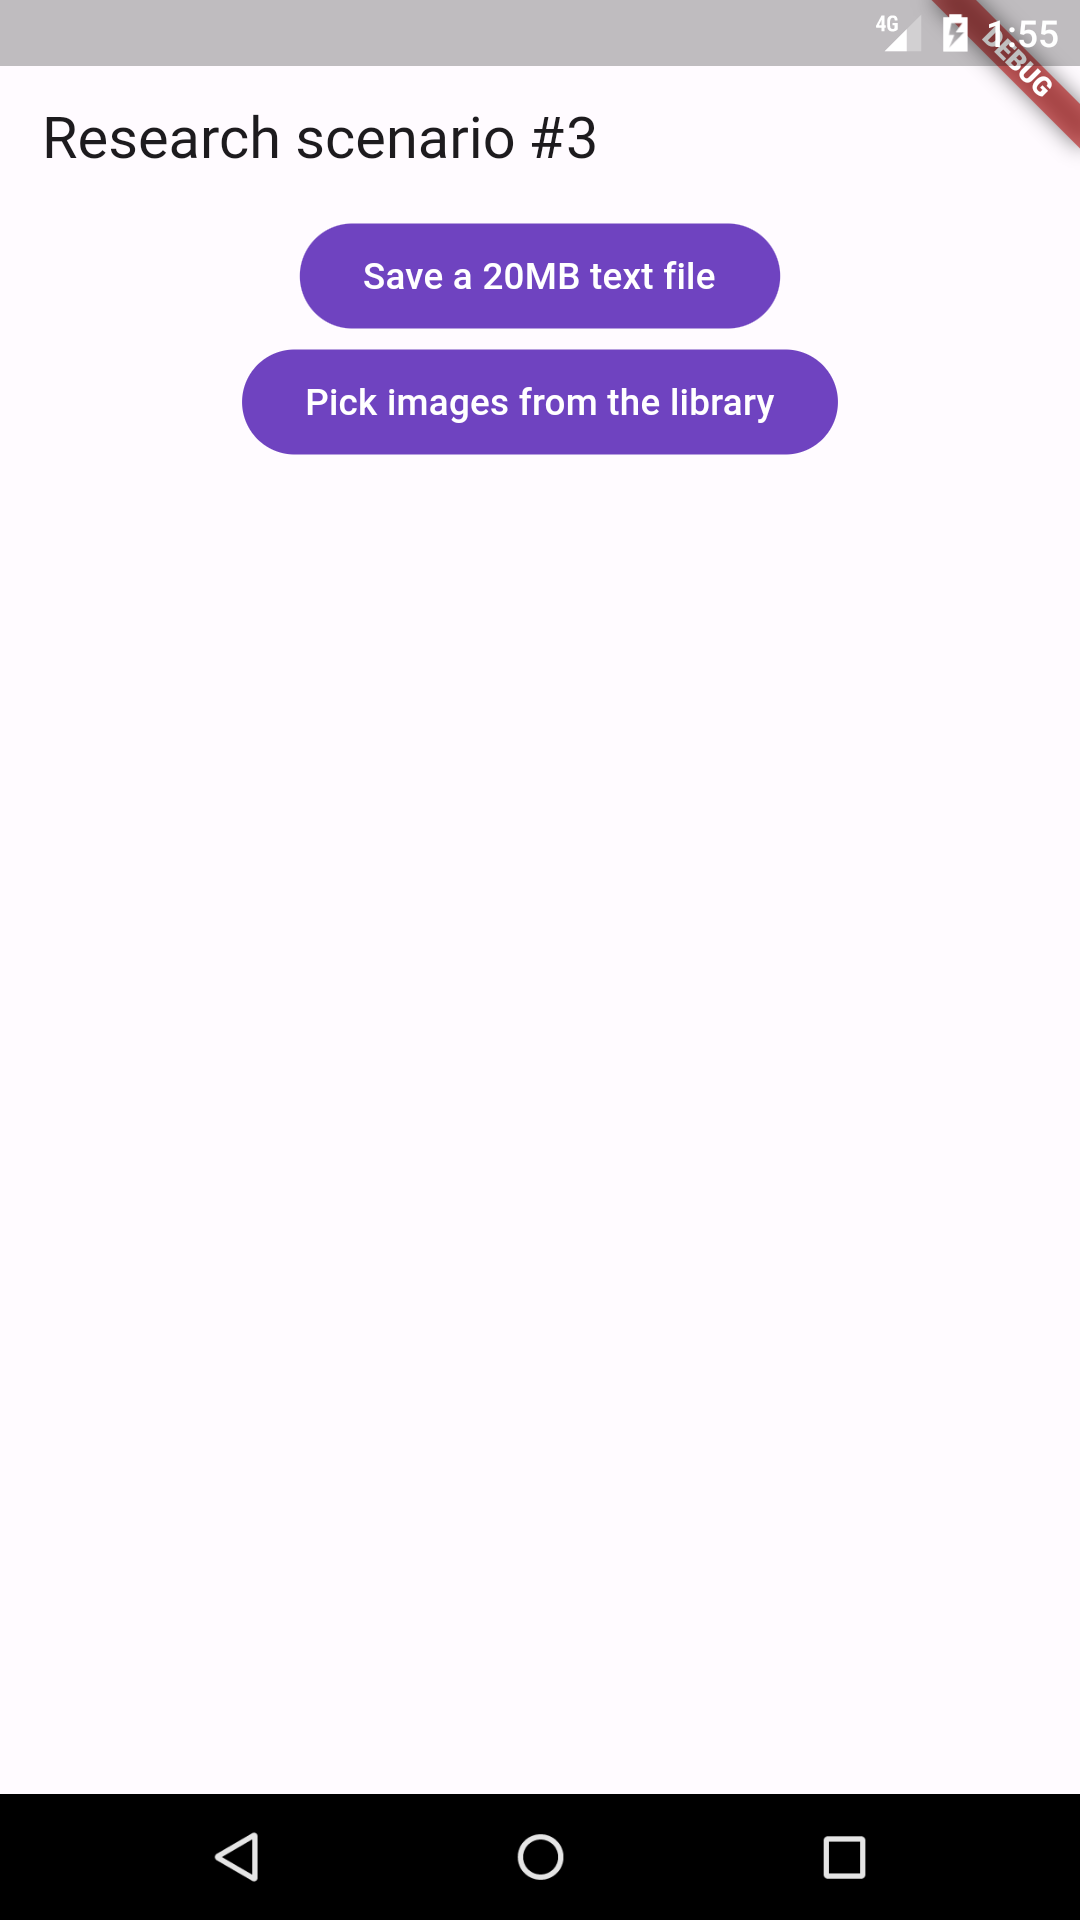
\includegraphics[height=50mm]{img/app3_flutter_android}
  \caption{App 3: Flutter Android (Source: Own work)}
  \label{fig:app3_flutter_android}
\end{minipage}
\hfill
\begin{minipage}{.47\textwidth}
  \centering
  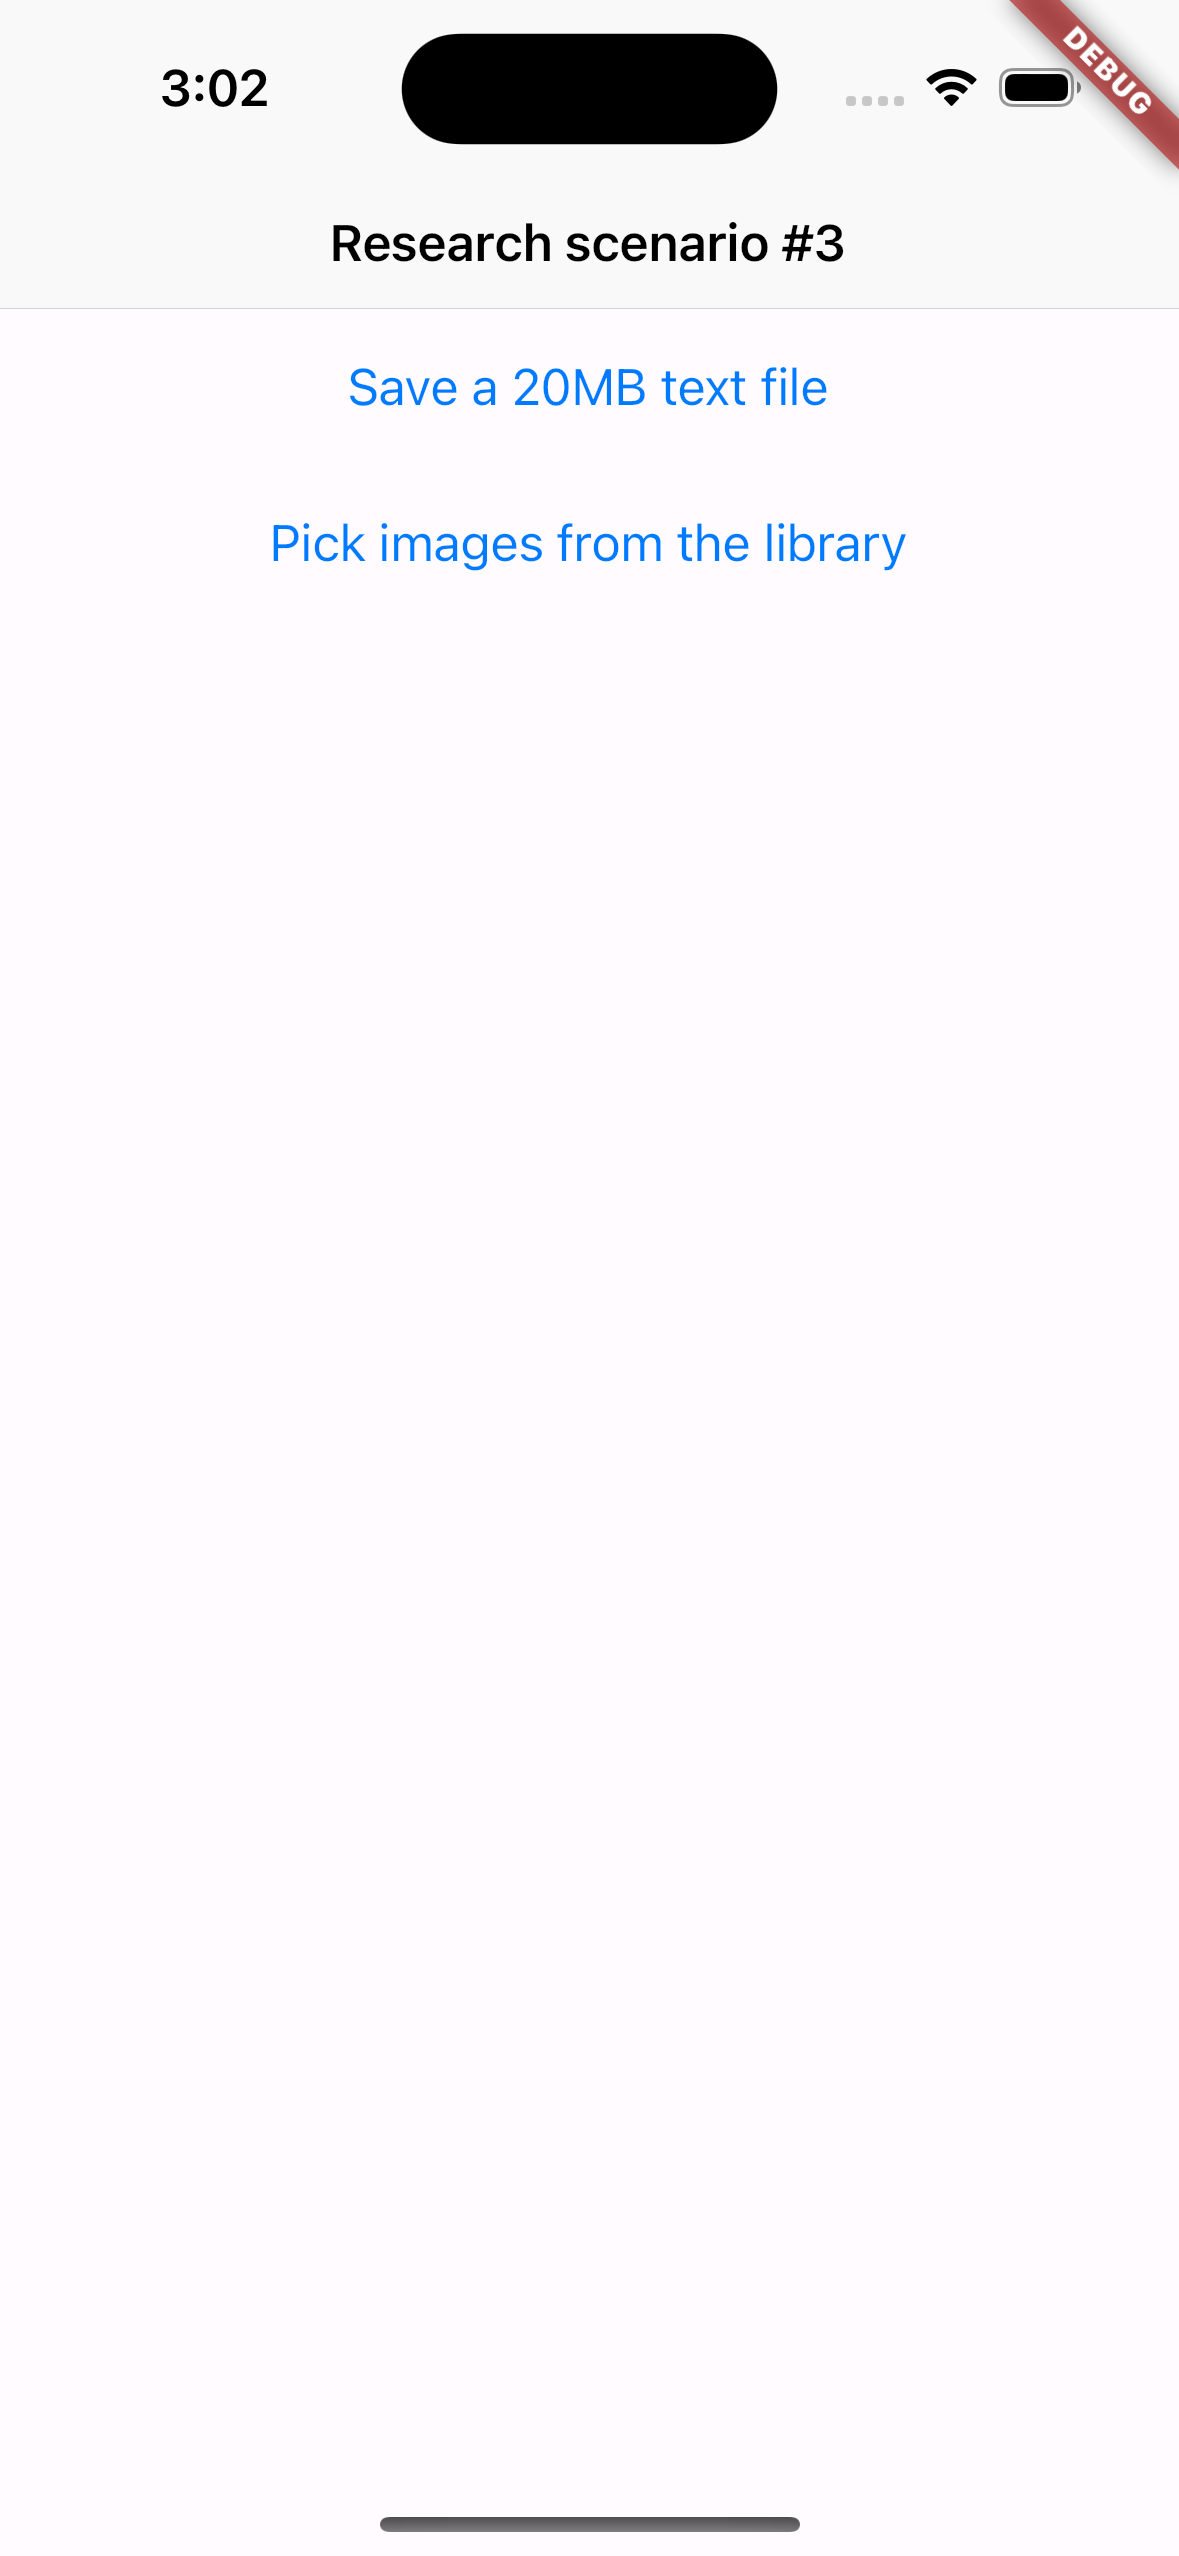
\includegraphics[height=50mm]{img/app3_flutter_ios}
  \caption{App 3: Flutter iOS (Source: Own work)}
  \label{fig:app3_flutter_ios}
\end{minipage}
\end{figure}

\begin{figure}[H]
\begin{minipage}{.47\textwidth}
  \centering
  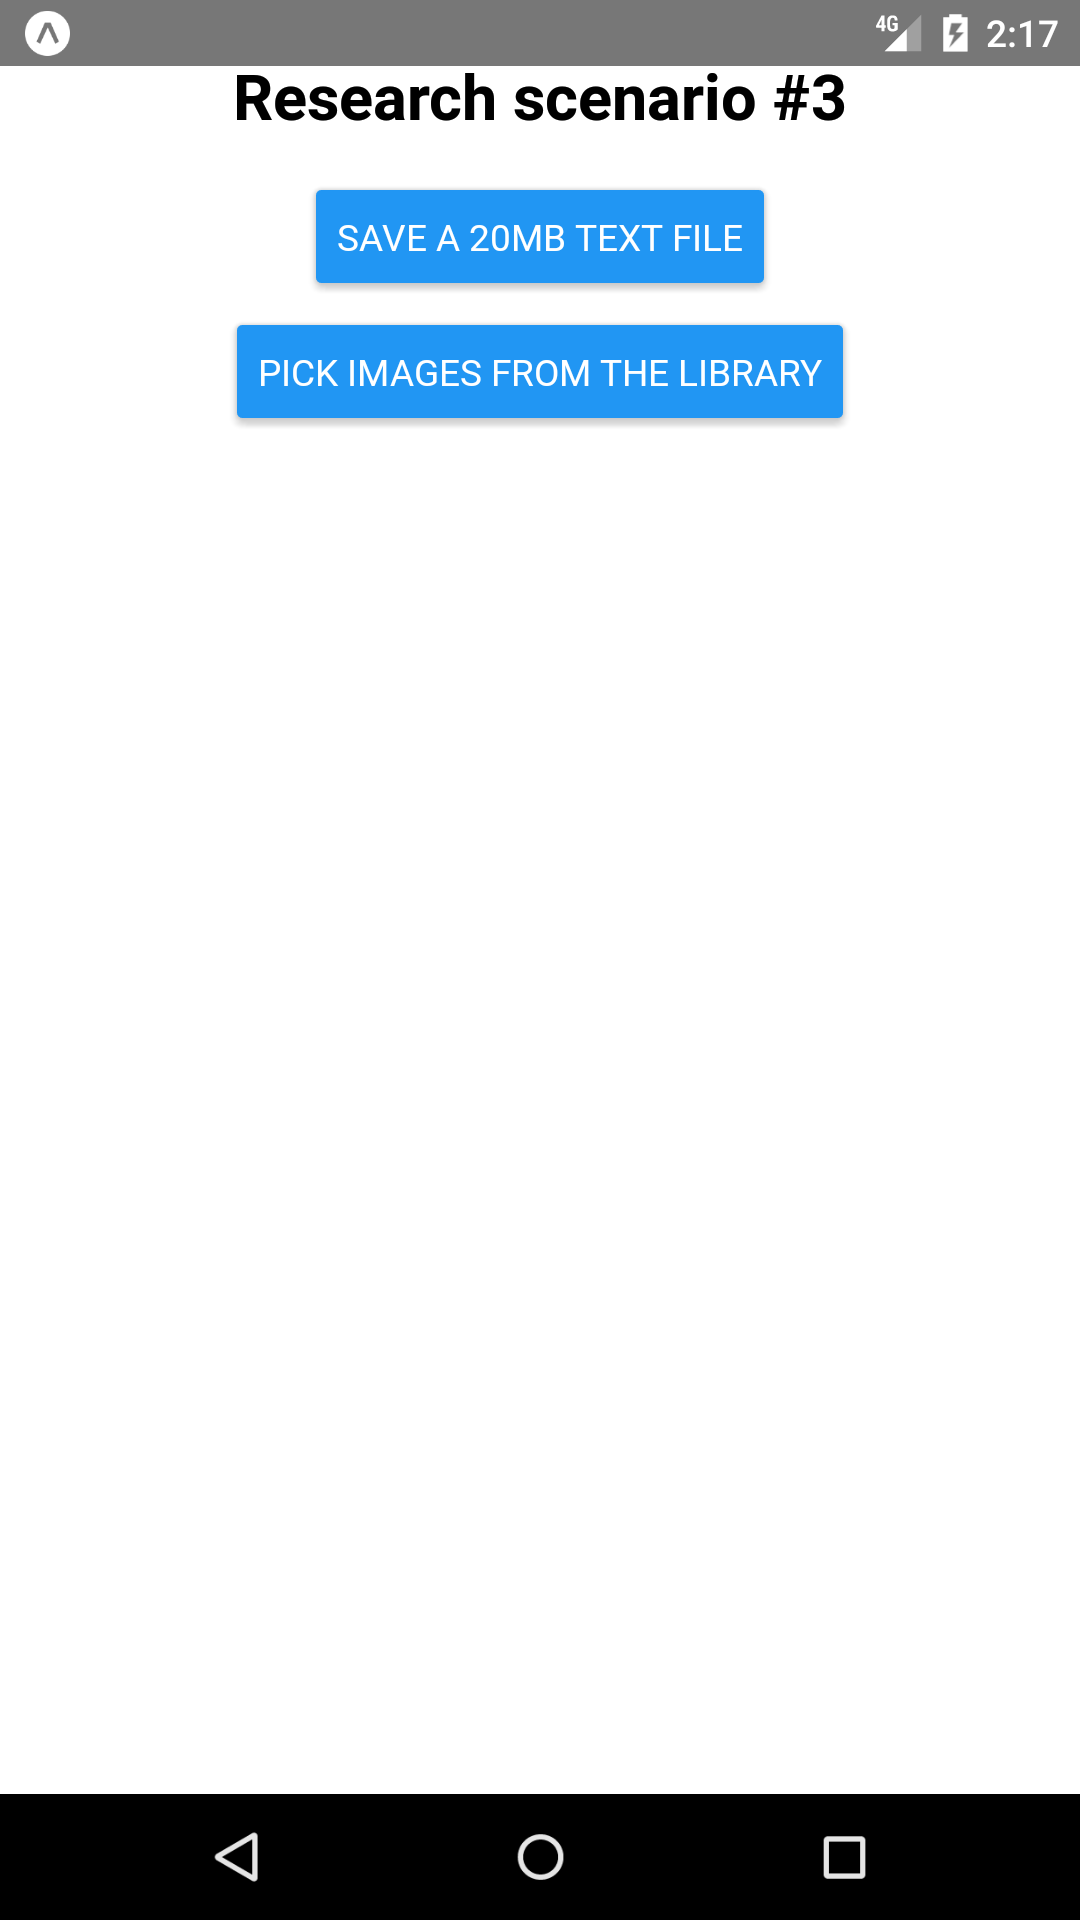
\includegraphics[height=50mm]{img/app3_rn_android}
  \caption{App 3: React Native Android (Source: Own work)}
  \label{fig:app3_rn_android}
\end{minipage}
\hfill
\begin{minipage}{.47\textwidth}
  \centering
  \frame{
    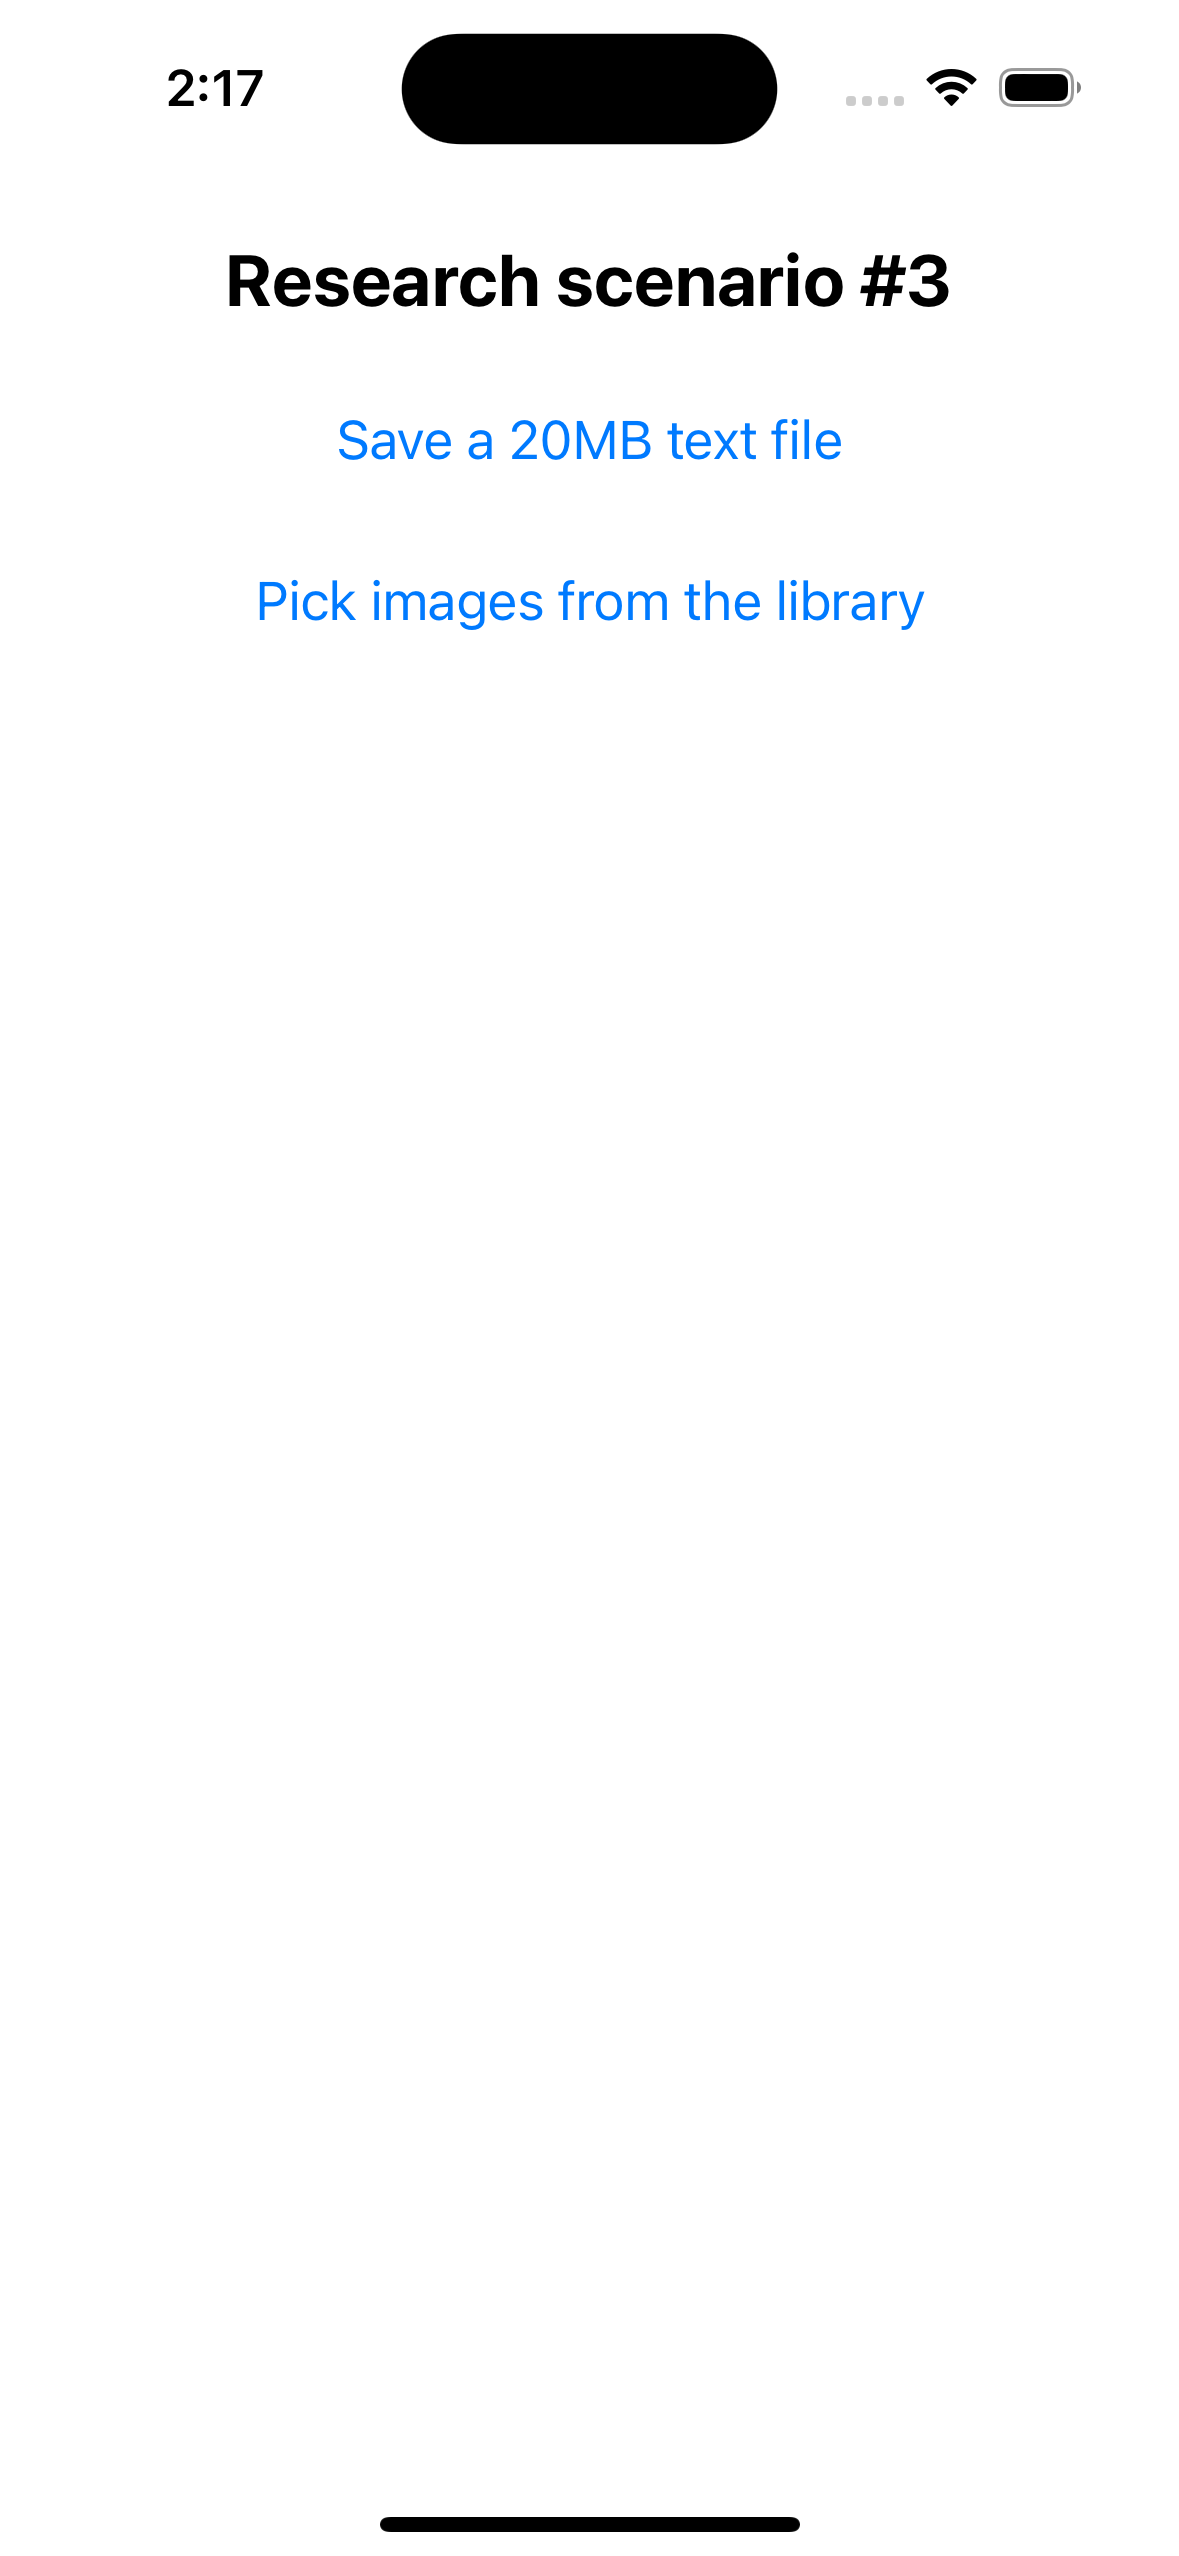
\includegraphics[height=50mm]{img/app3_rn_ios}
  }
  \caption{App 3: React Native iOS (Source: Own work)}
  \label{fig:app3_rn_ios}
\end{minipage}
\end{figure}

\section{Research scenario 4: Common UI elements}

The application consists of three views: \emph{Controls Page}, \emph{Form Page} and \emph{External Page}. Various common UI components are utilized as well as the bottom tab bar navigation.

\begin{figure}[H]
  \begin{minipage}{.31\textwidth}
    \centering
    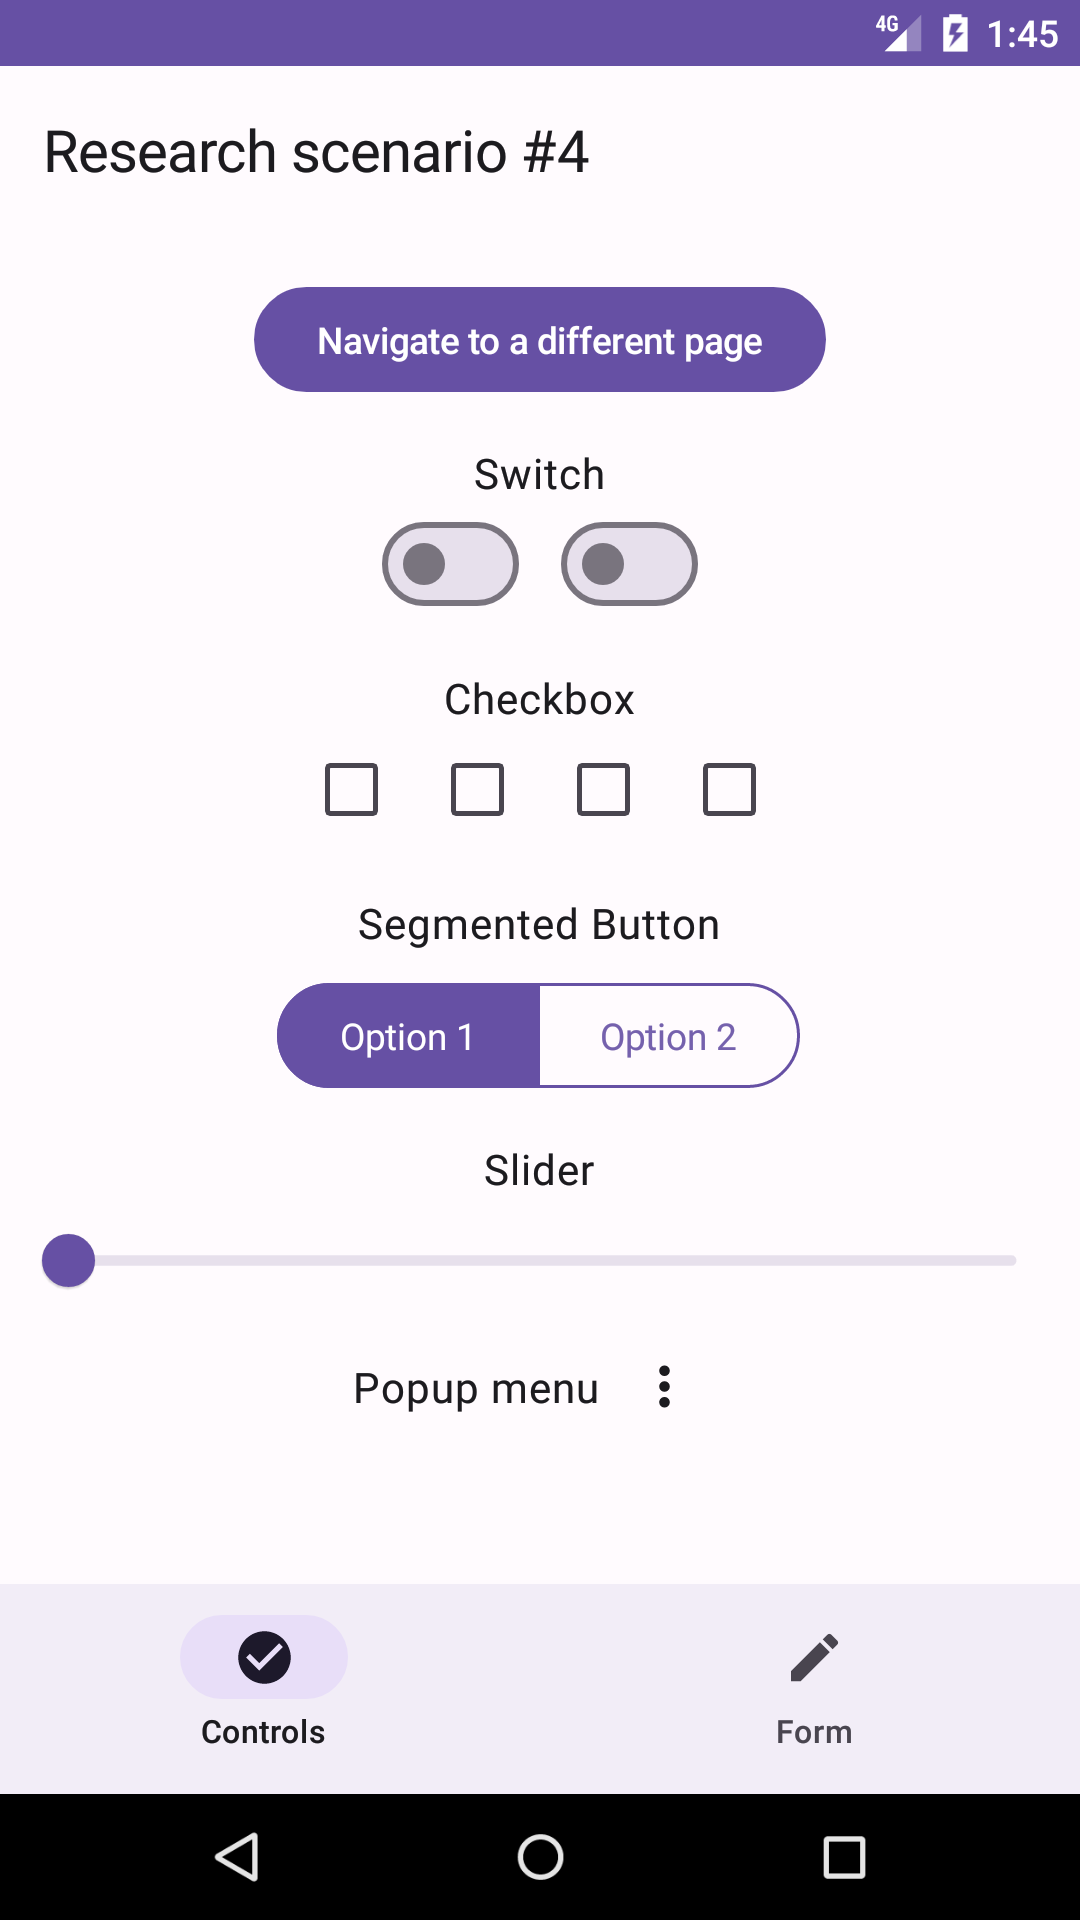
\includegraphics[height=50mm]{img/app4_1_kotlin}
    \caption{App 4 (1/3): Kotlin (Source: Own work)}
    \label{fig:app4_1_kotlin}
  \end{minipage}
  \hfill
  \begin{minipage}{.31\textwidth}
    \centering
    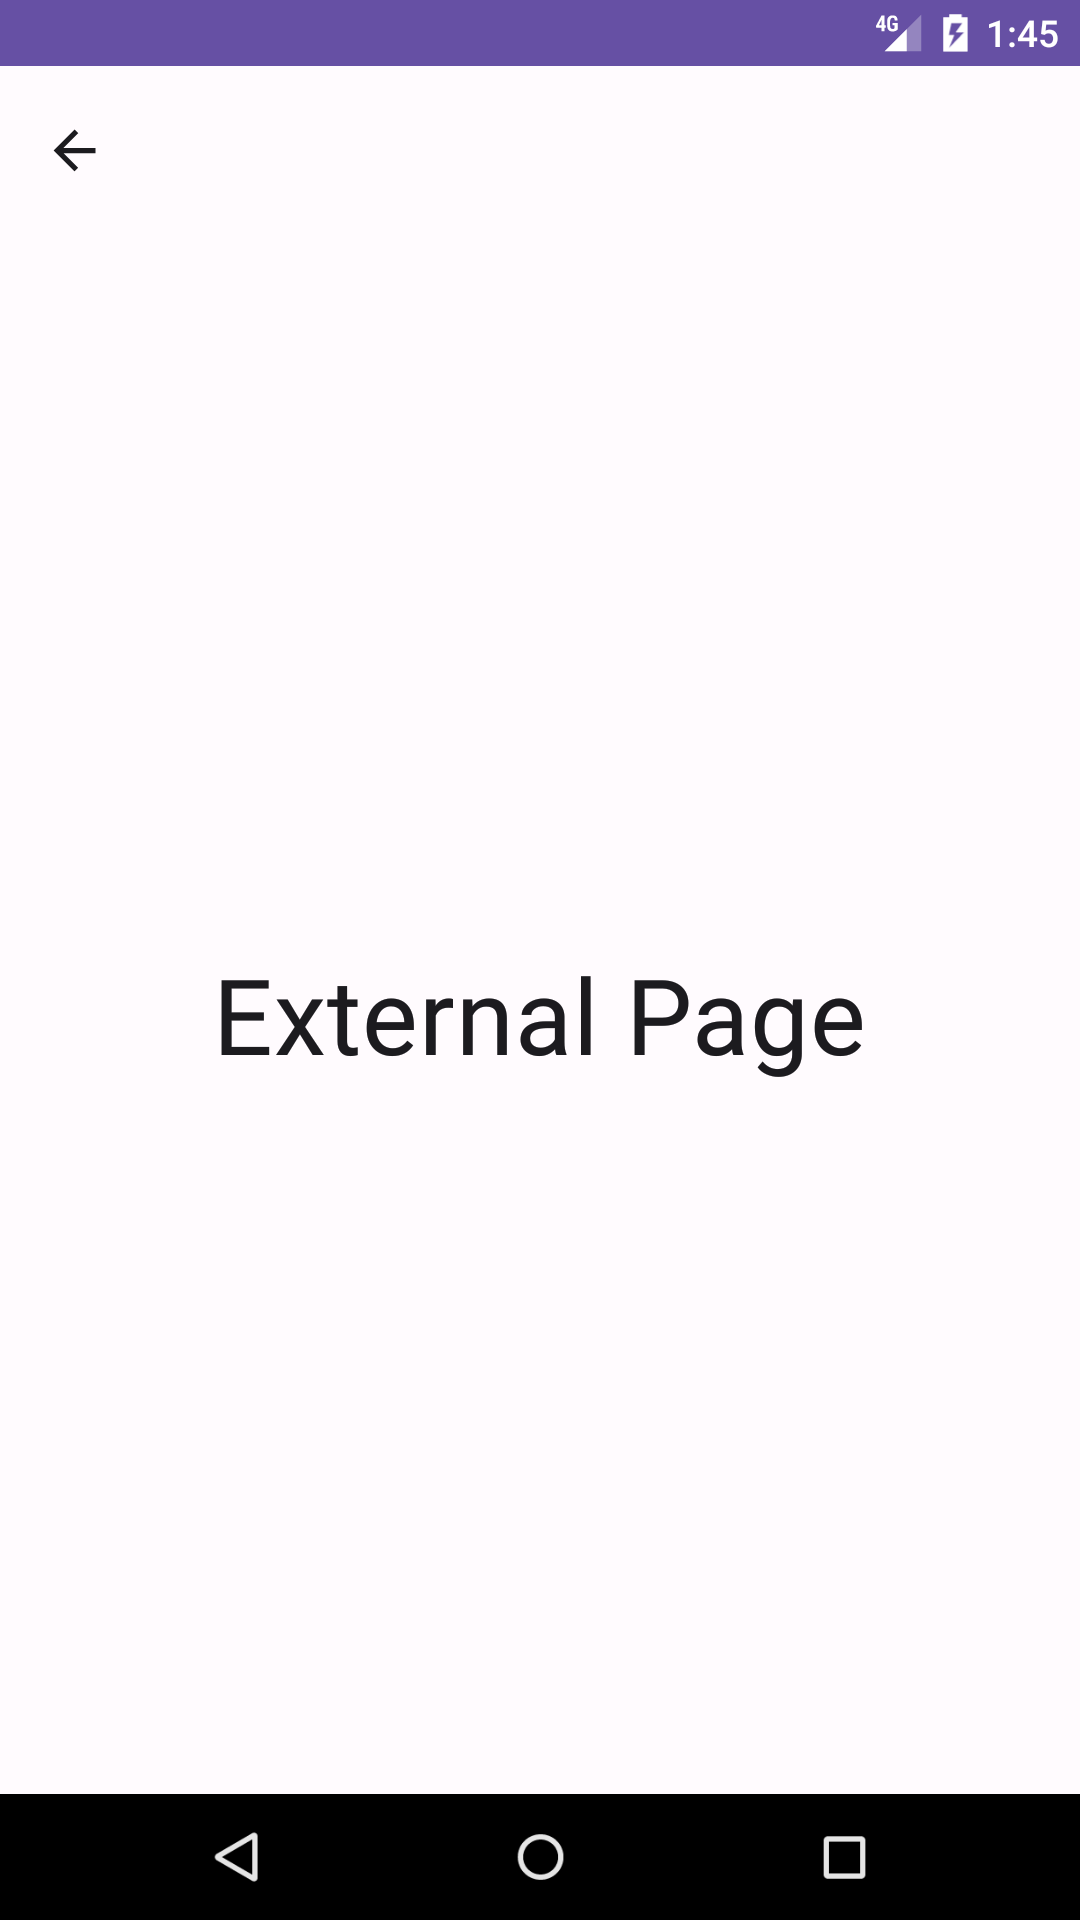
\includegraphics[height=50mm]{img/app4_2_kotlin}
    \caption{App 4 (2/3): Kotlin (Source: Own work)}
    \label{fig:app4_2_kotlin}
  \end{minipage}
  \hfill
  \begin{minipage}{.31\textwidth}
    \centering
    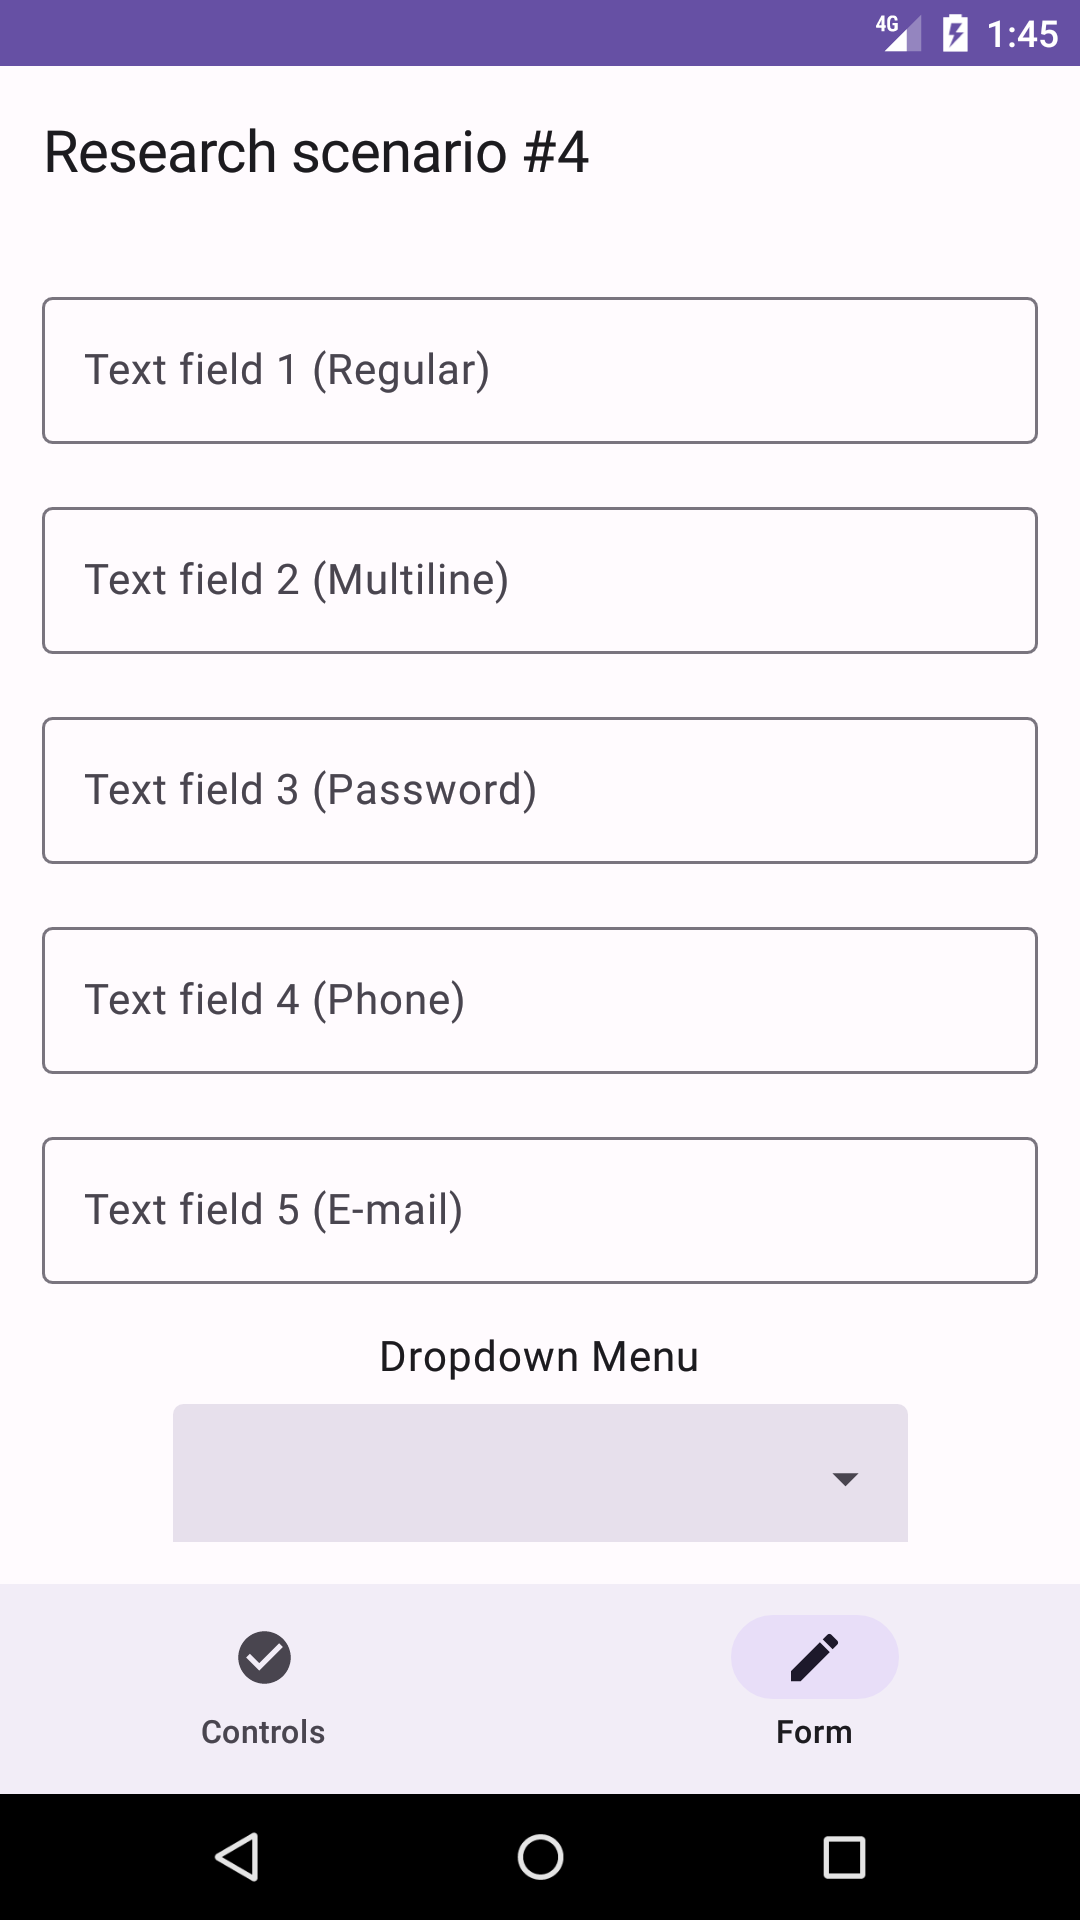
\includegraphics[height=50mm]{img/app4_3_kotlin}
    \caption{App 4 (3/3): Kotlin (Source: Own work)}
    \label{fig:app4_3_kotlin}
  \end{minipage}
\end{figure}

\begin{figure}[H]
  \begin{minipage}{.31\textwidth}
    \centering
    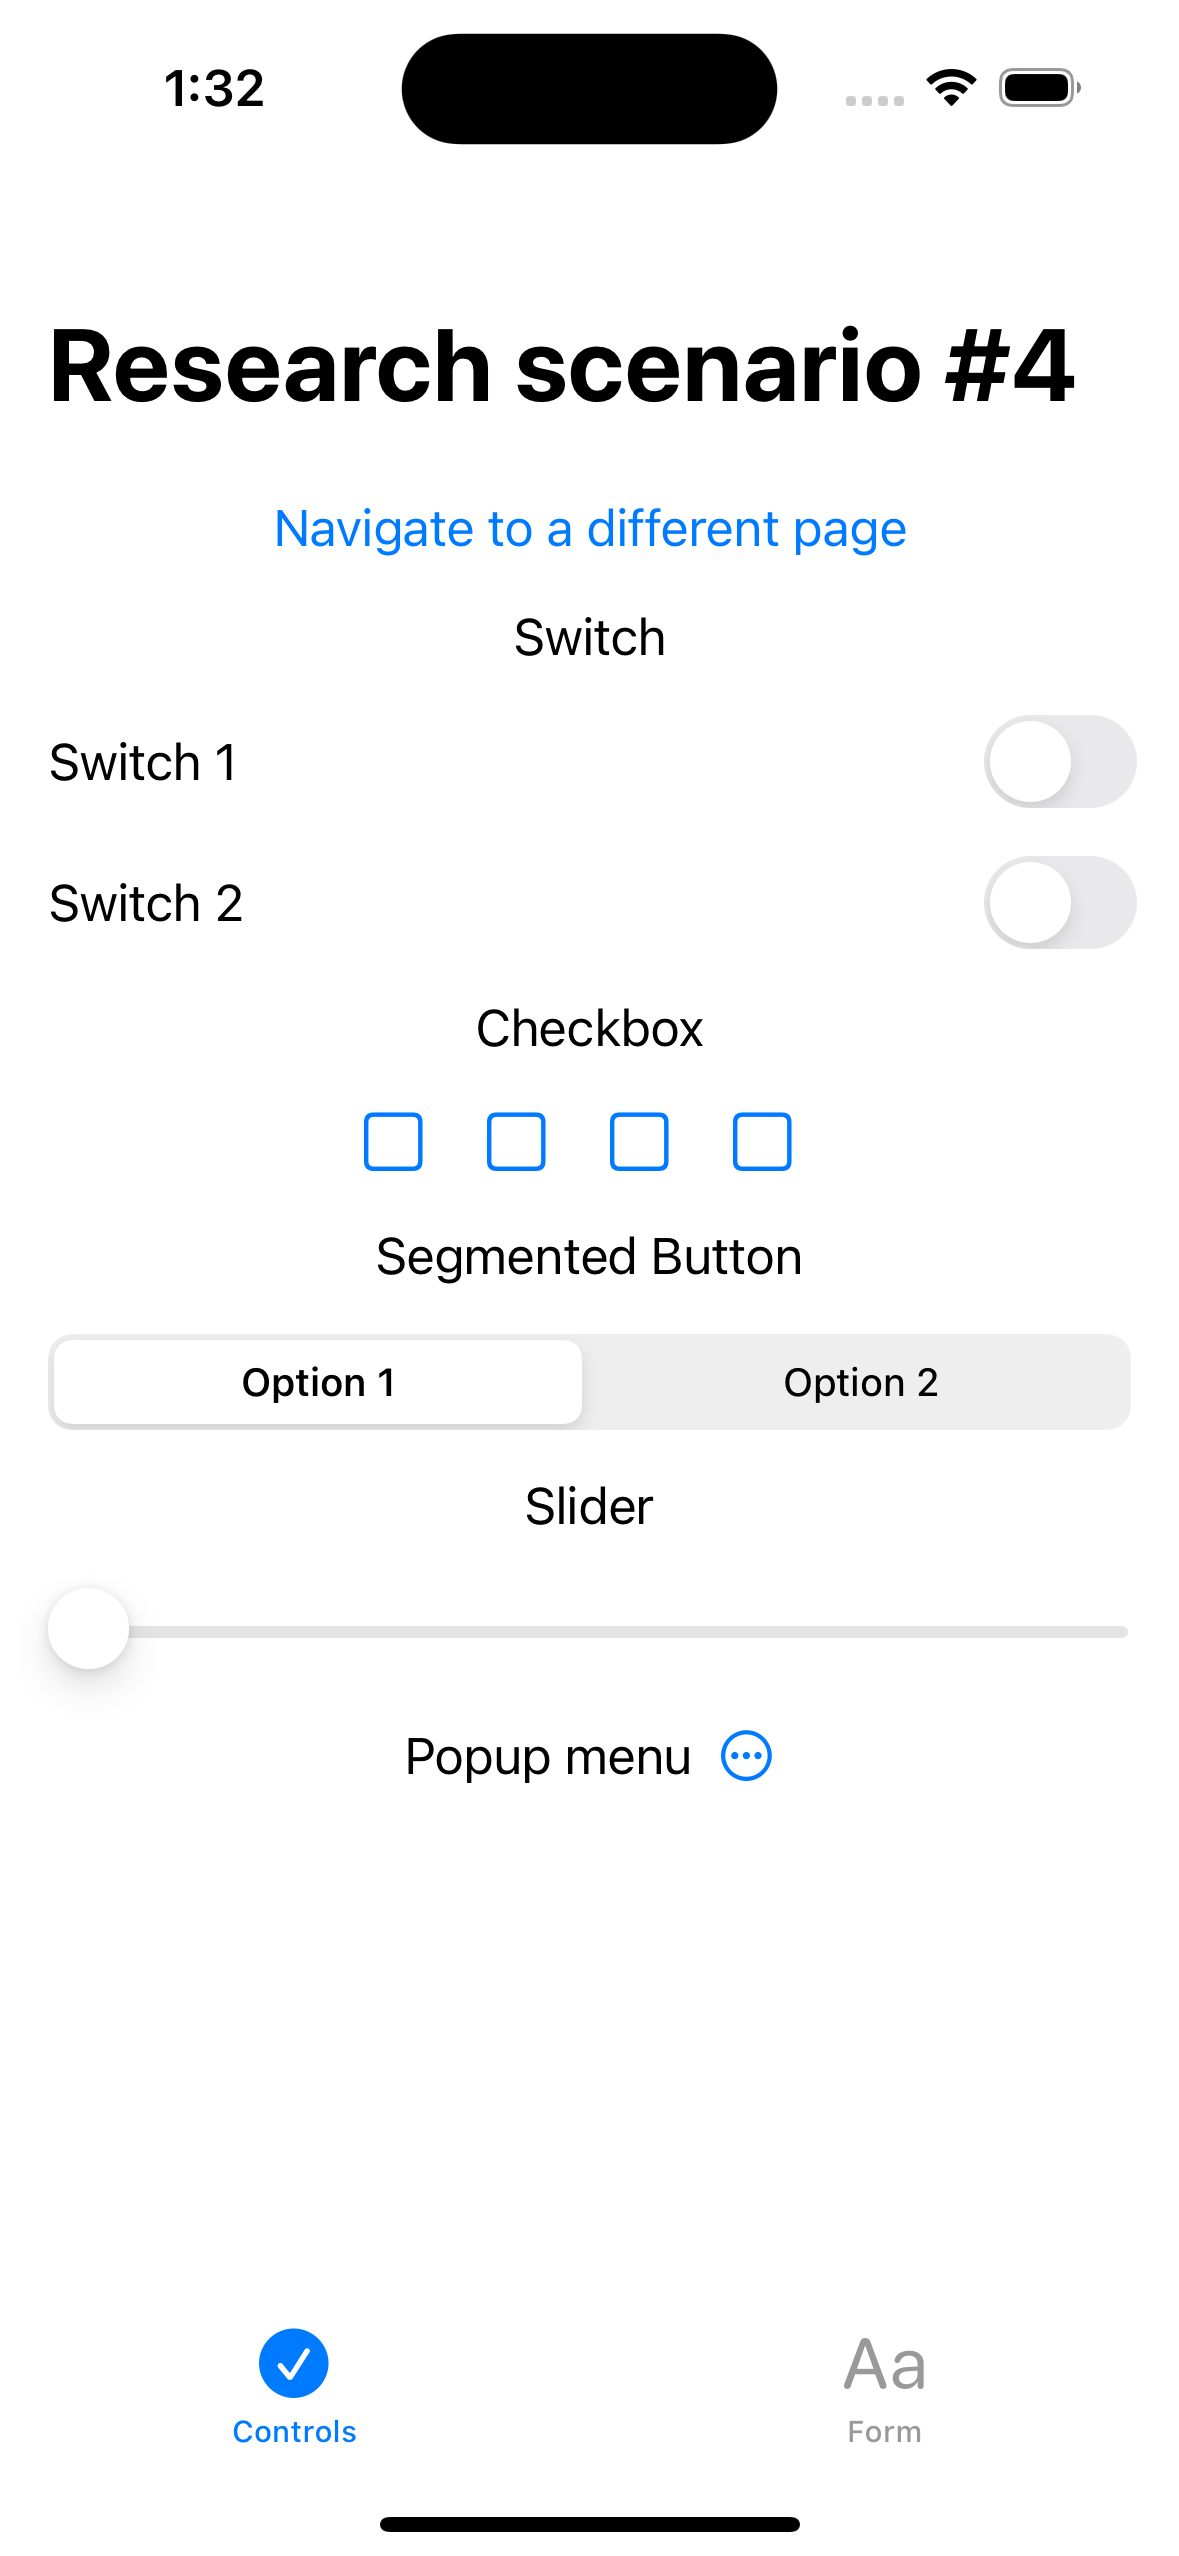
\includegraphics[height=50mm]{img/app4_1_swift}
    \caption{App 4 (1/3): Swift (Source: Own work)}
    \label{fig:app4_1_swift}
  \end{minipage}
  \hfill
  \begin{minipage}{.31\textwidth}
    \centering
    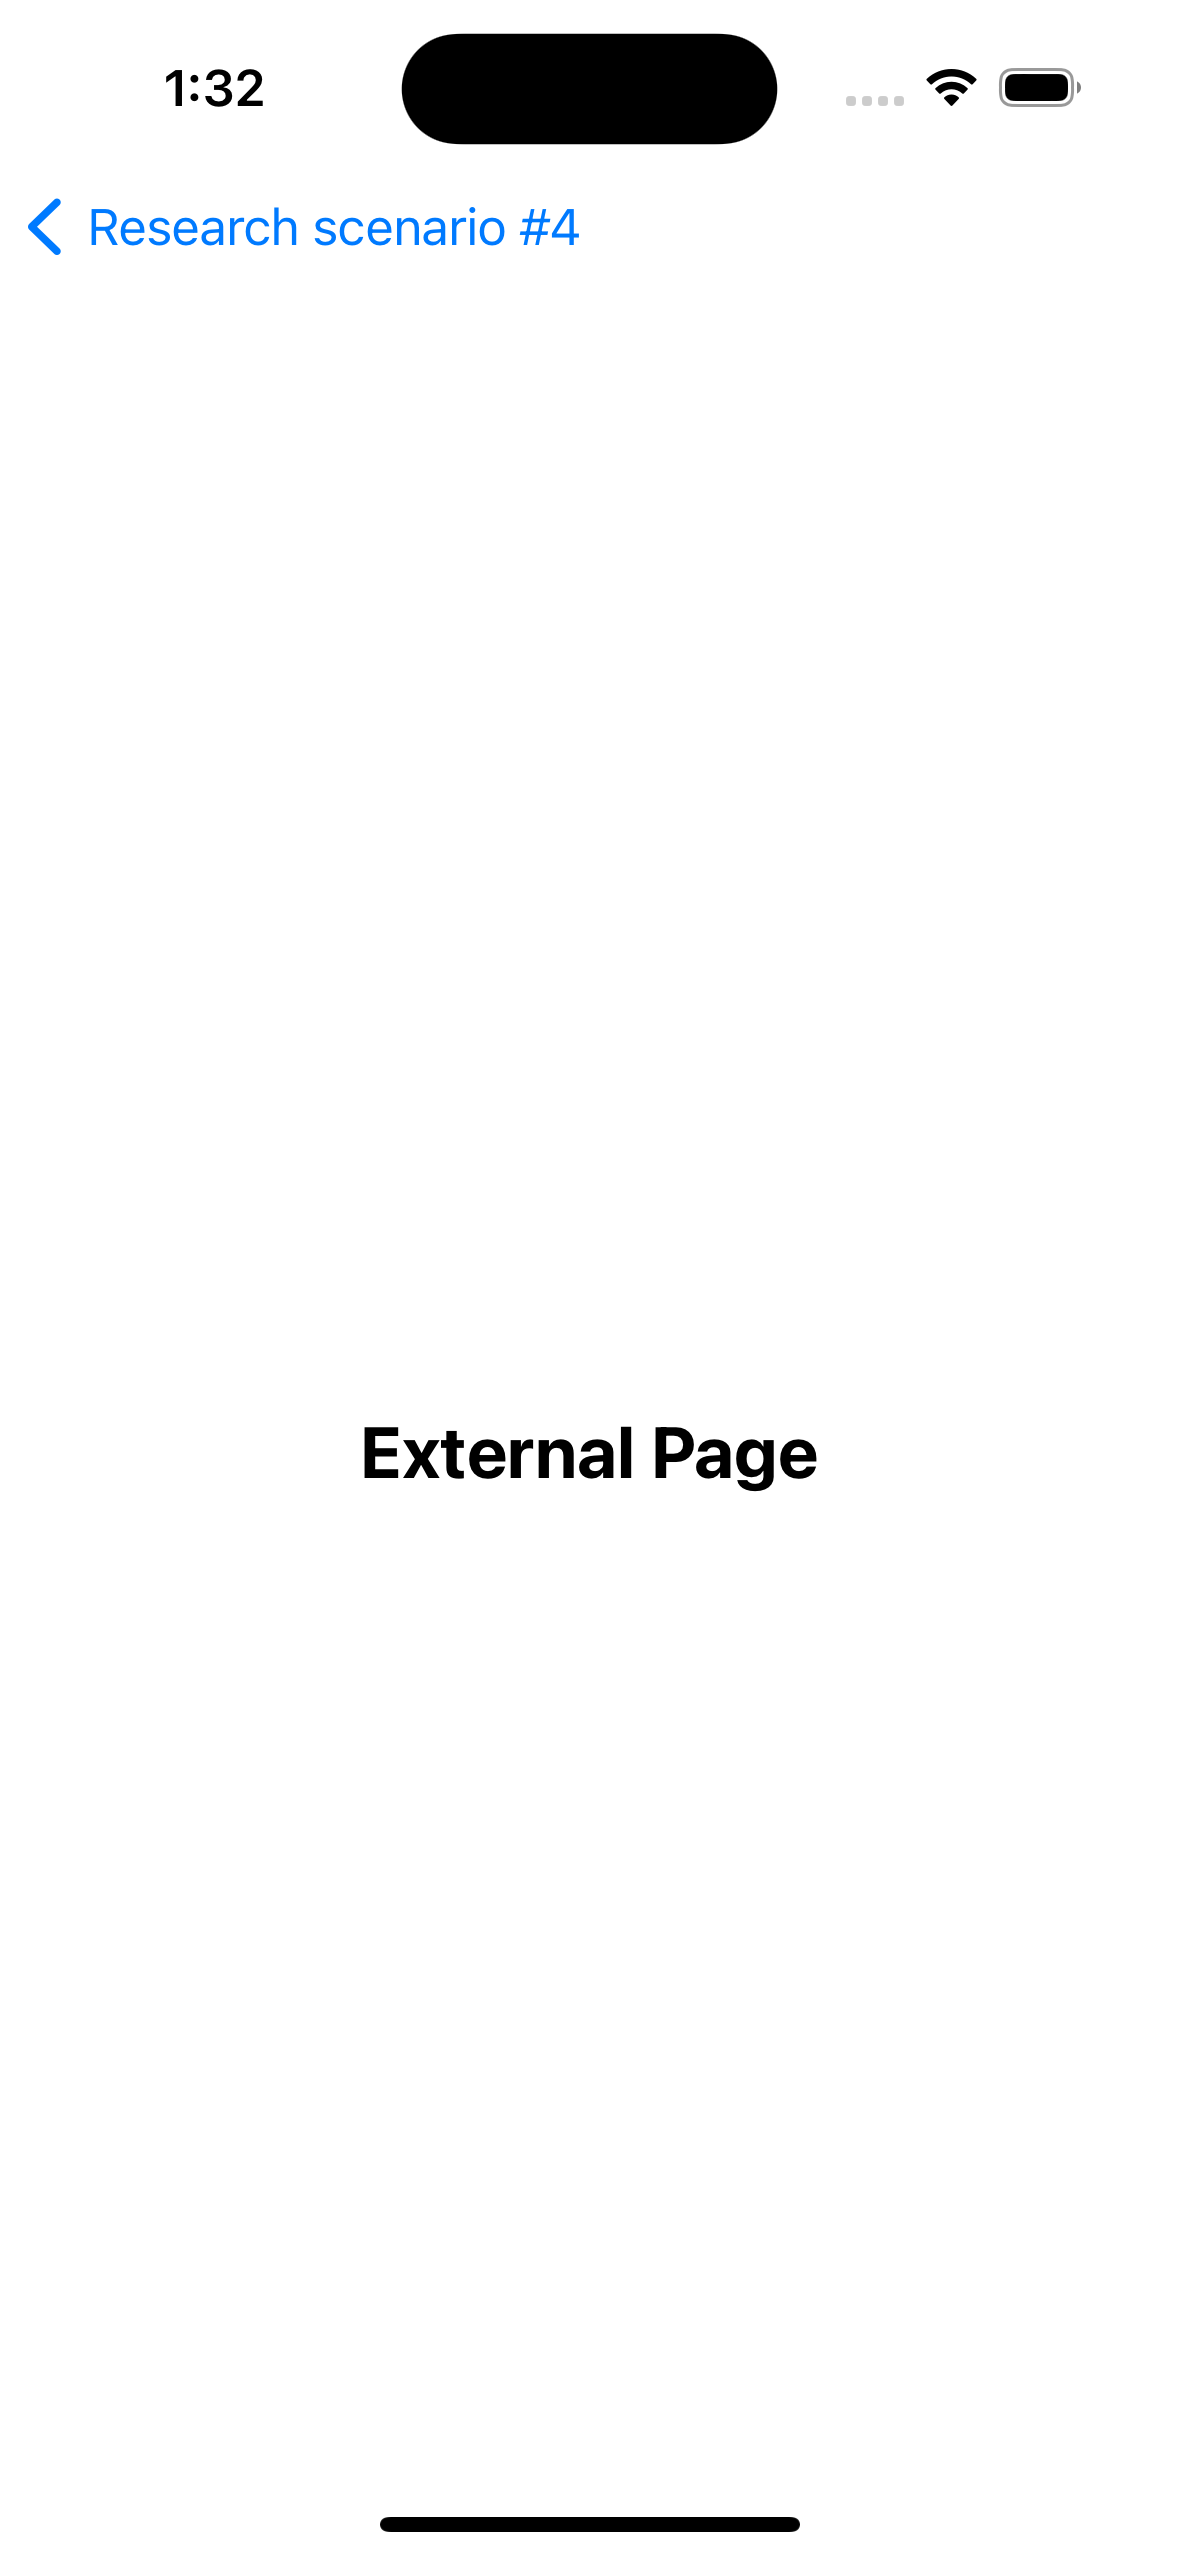
\includegraphics[height=50mm]{img/app4_2_swift}
    \caption{App 4 (2/3): Swift (Source: Own work)}
    \label{fig:app4_2_swift}
  \end{minipage}
  \hfill
  \begin{minipage}{.31\textwidth}
    \centering
    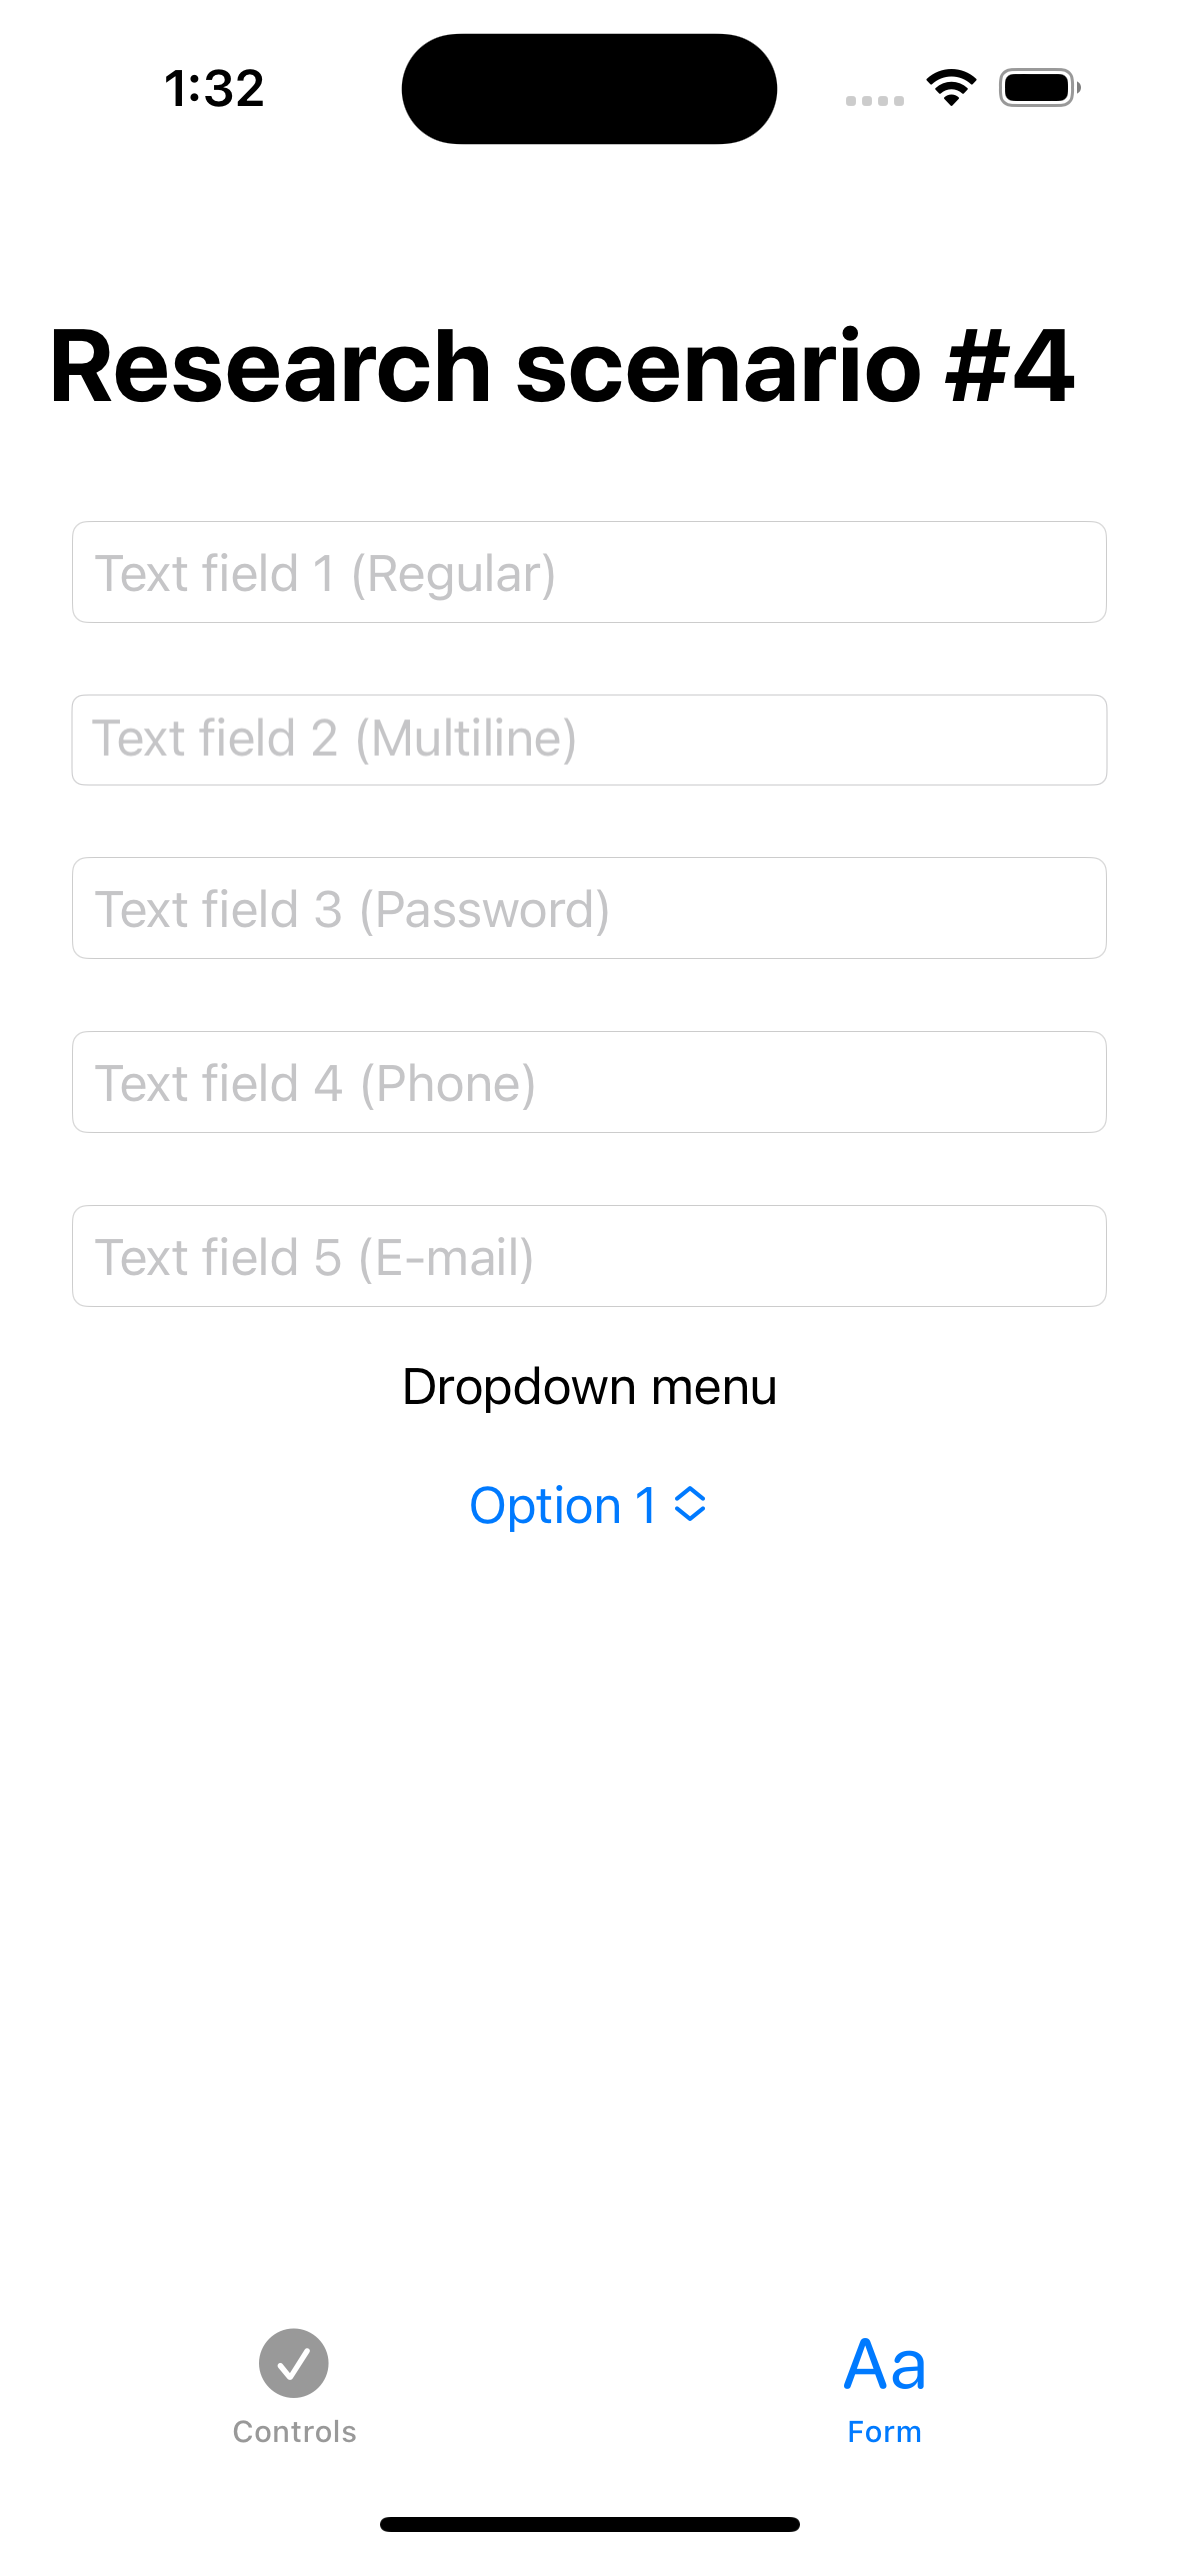
\includegraphics[height=50mm]{img/app4_3_swift}
    \caption{App 4 (3/3): Swift (Source: Own work)}
    \label{fig:app4_3_swift}
  \end{minipage}
\end{figure}

\begin{figure}[H]
  \begin{minipage}{.31\textwidth}
    \centering
    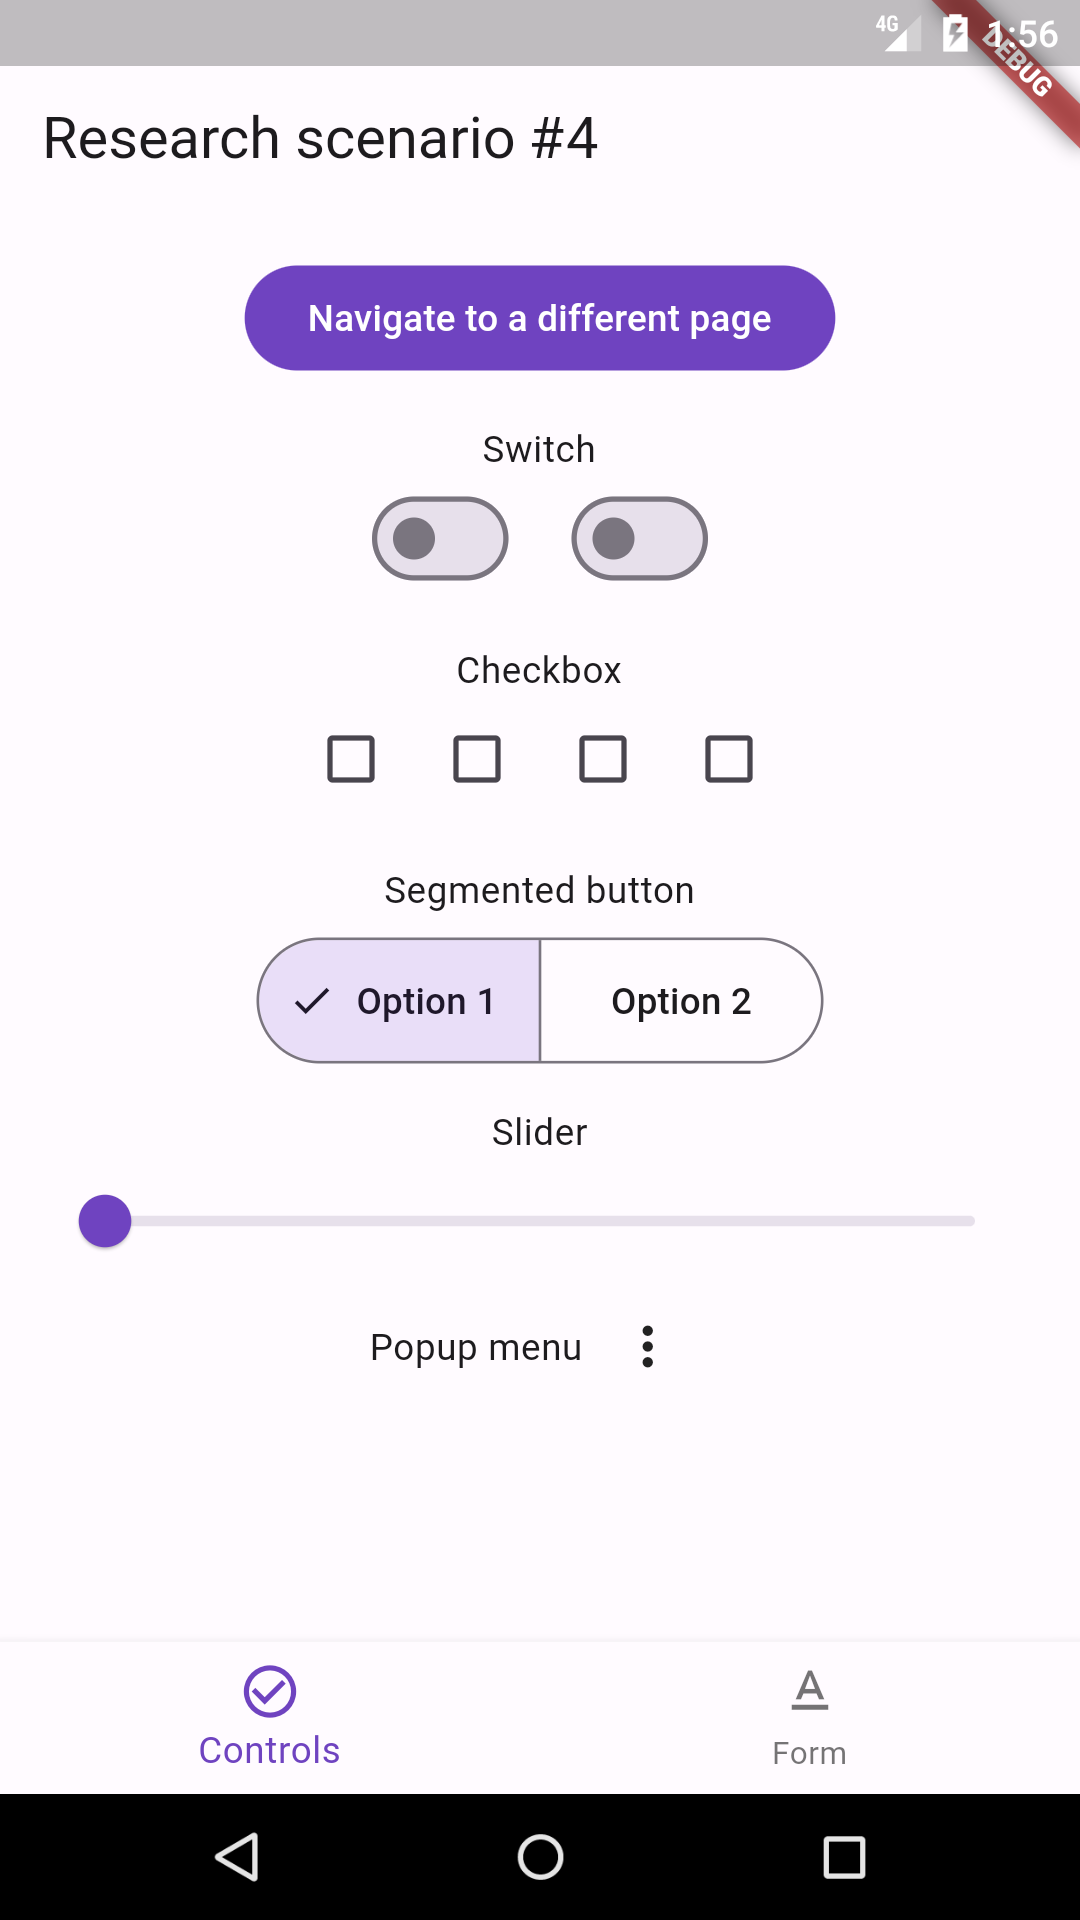
\includegraphics[height=50mm]{img/app4_1_flutter_android}
    \caption{App 4 (1/3): Flutter Android (Source: Own work)}
    \label{fig:app4_1_flutter_android}
  \end{minipage}
  \hfill
  \begin{minipage}{.31\textwidth}
    \centering
    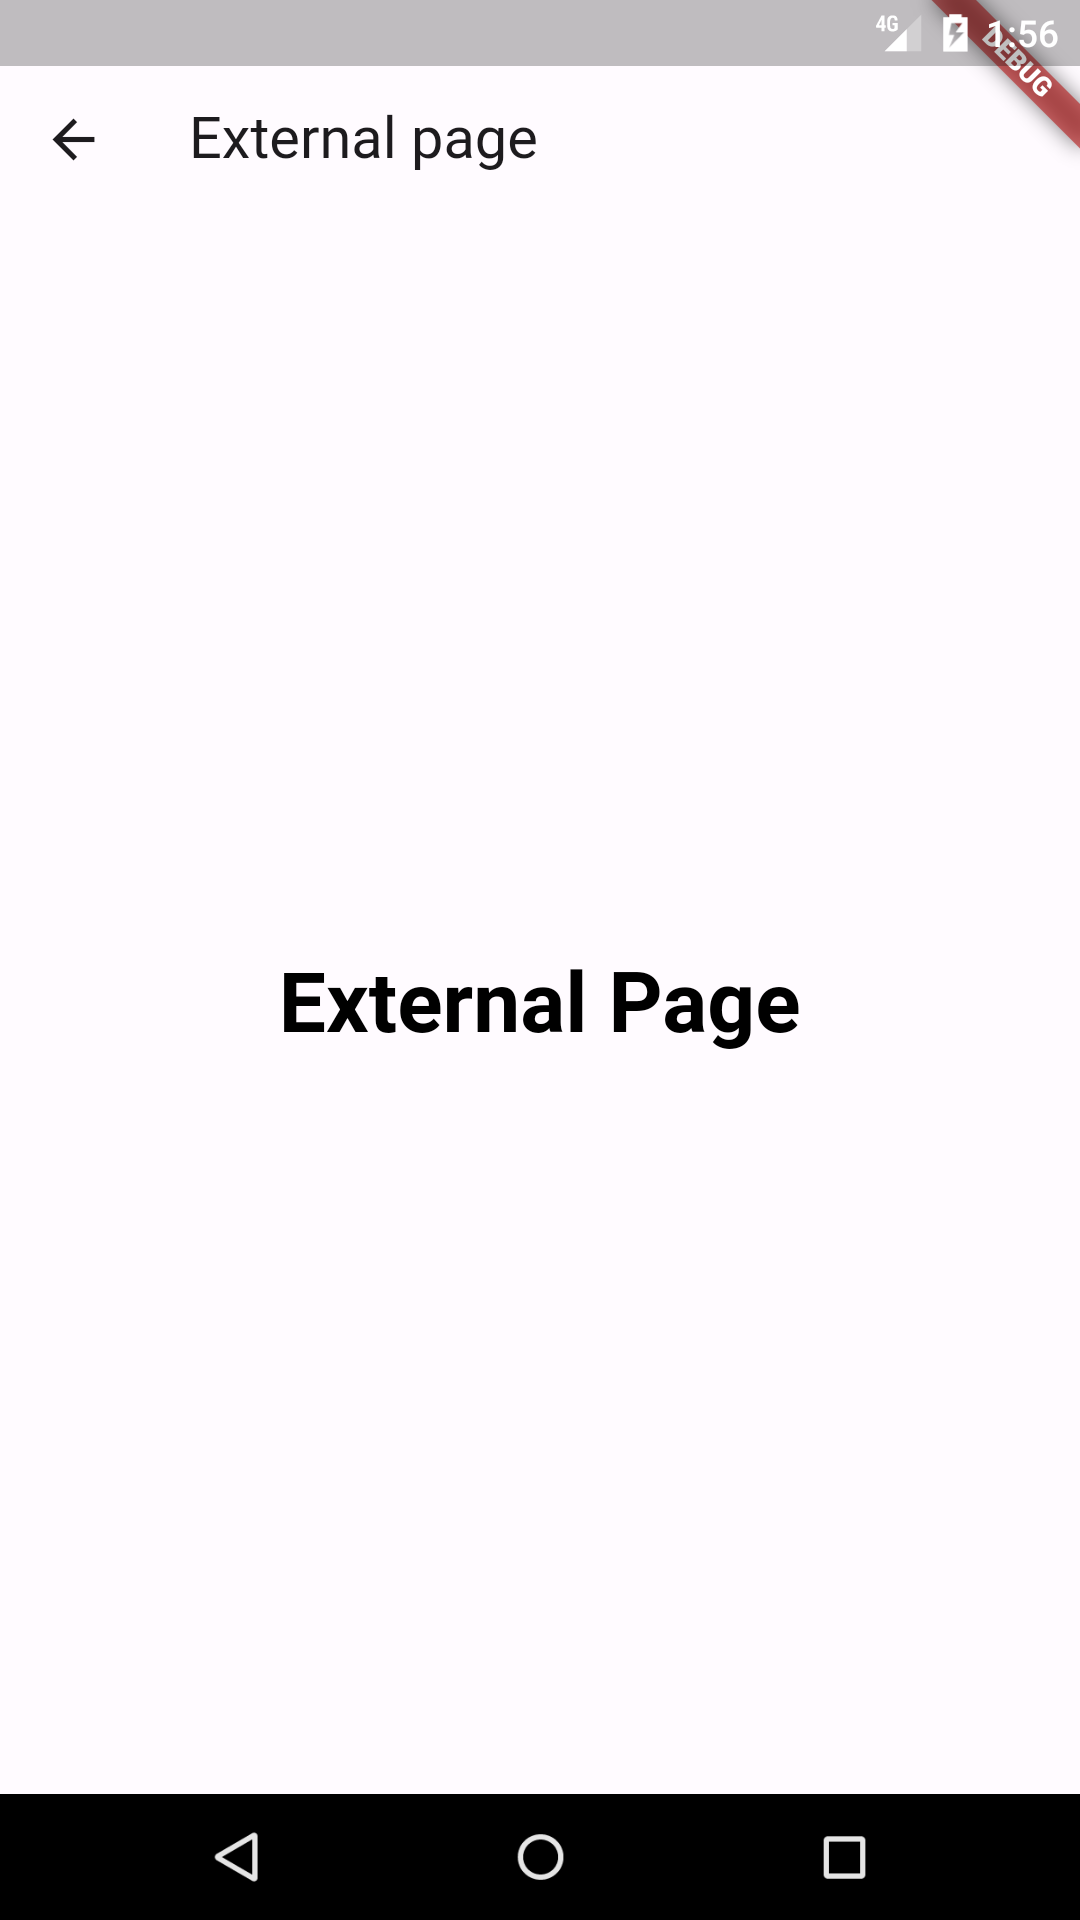
\includegraphics[height=50mm]{img/app4_2_flutter_android}
    \caption{App 4 (2/3): Flutter Android (Source: Own work)}
    \label{fig:app4_2_flutter_android}
  \end{minipage}
  \hfill
  \begin{minipage}{.31\textwidth}
    \centering
    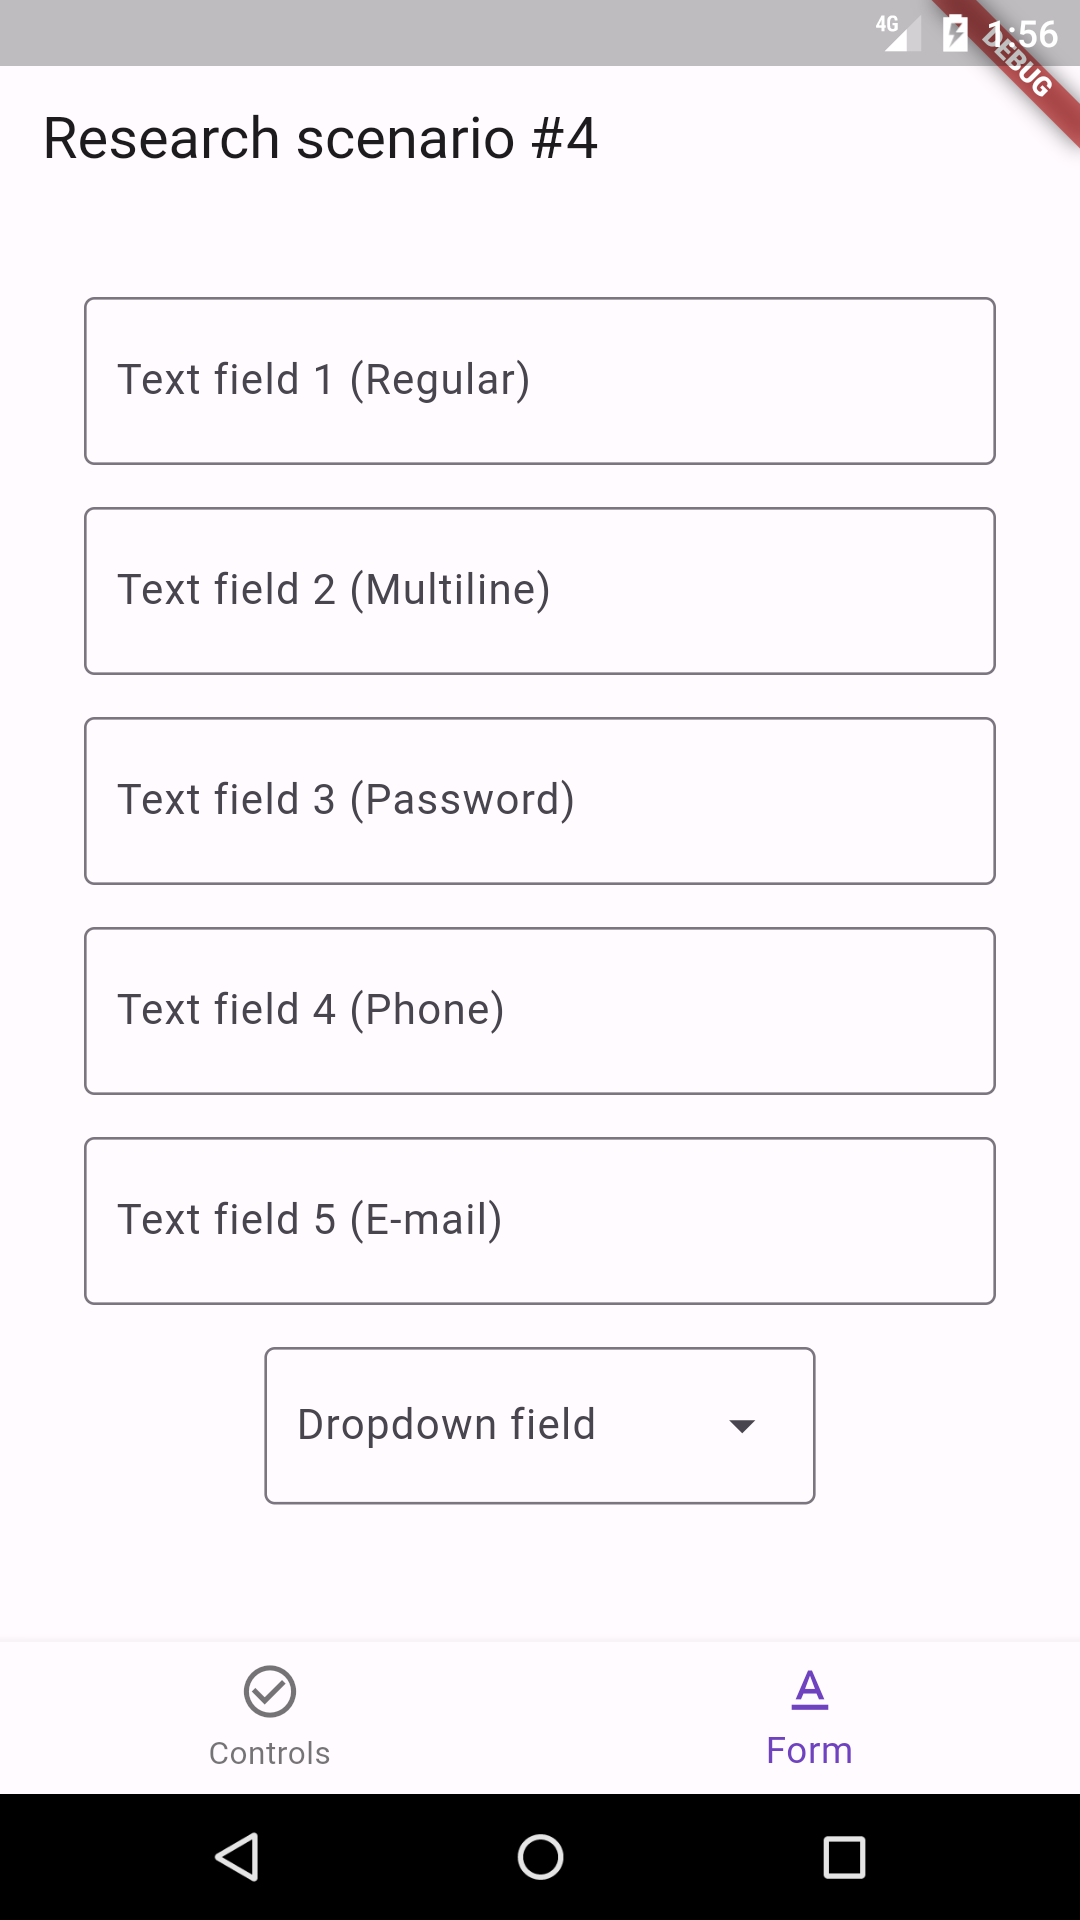
\includegraphics[height=50mm]{img/app4_3_flutter_android}
    \caption{App 4 (3/3): Flutter Android (Source: Own work)}
    \label{fig:app4_3_flutter_android}
  \end{minipage}
\end{figure}

\begin{figure}[H]
  \begin{minipage}{.31\textwidth}
    \centering
    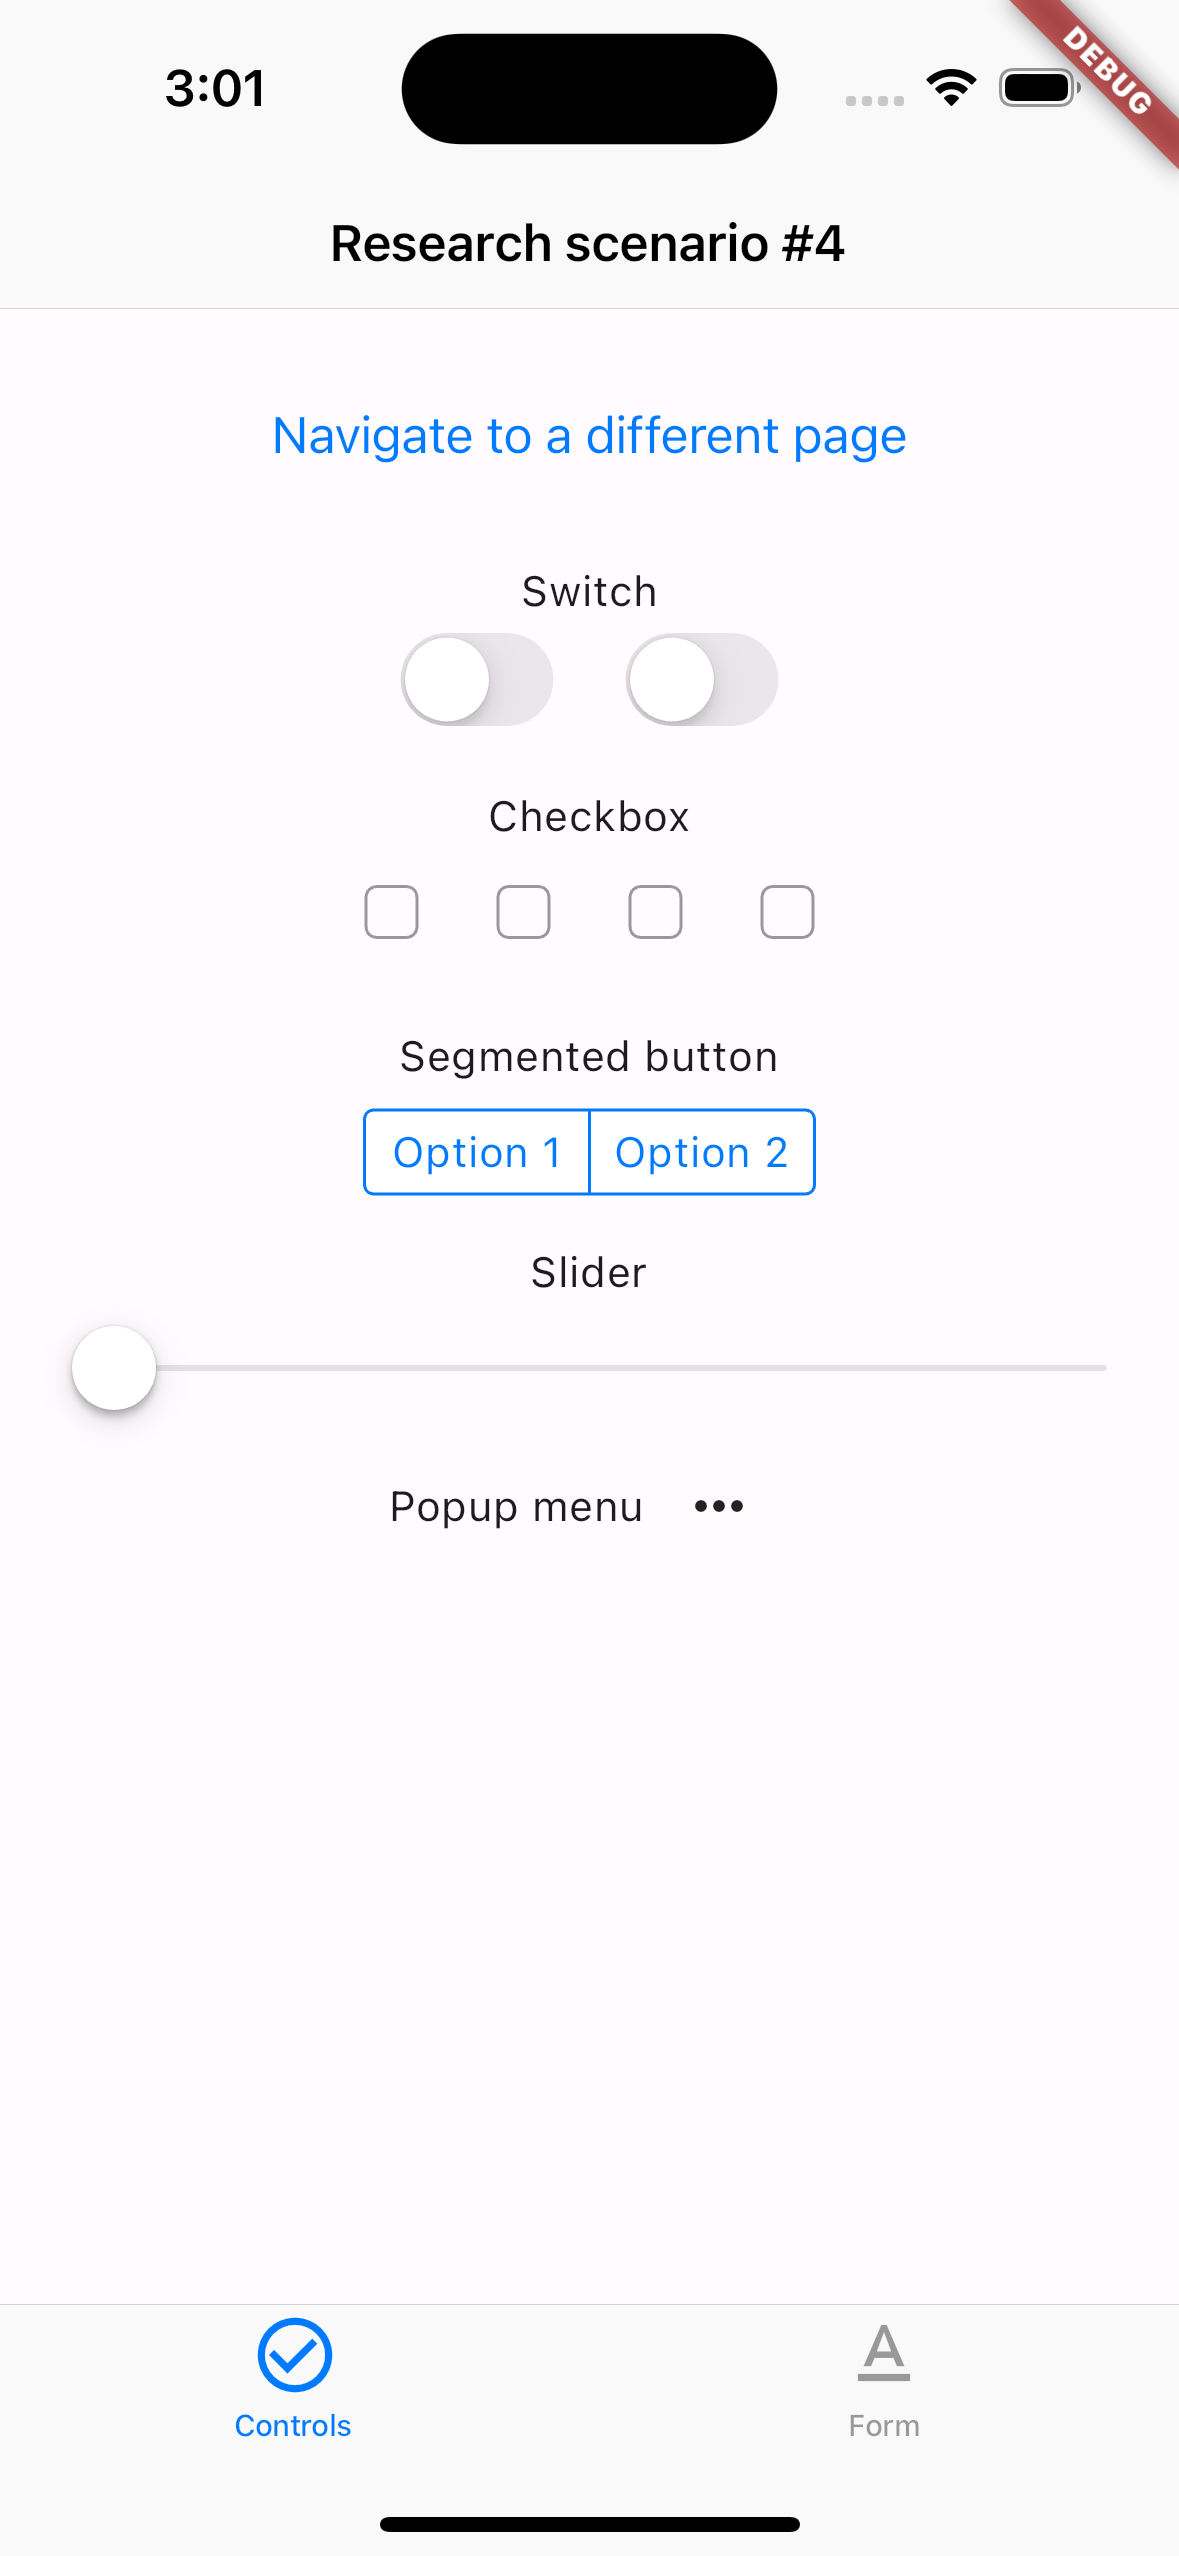
\includegraphics[height=50mm]{img/app4_1_flutter_ios}
    \caption{App 4 (1/3): Flutter iOS (Source: Own work)}
    \label{fig:app4_1_flutter_ios}
  \end{minipage}
  \hfill
  \begin{minipage}{.31\textwidth}
    \centering
    
\includegraphics[height=50mm]{img/app4_2_flutter_ios}
    \caption{App 4 (2/3): Flutter iOS (Source: Own work)}
    \label{fig:app4_2_flutter_ios}
  \end{minipage}
  \hfill
  \begin{minipage}{.31\textwidth}
    \centering
    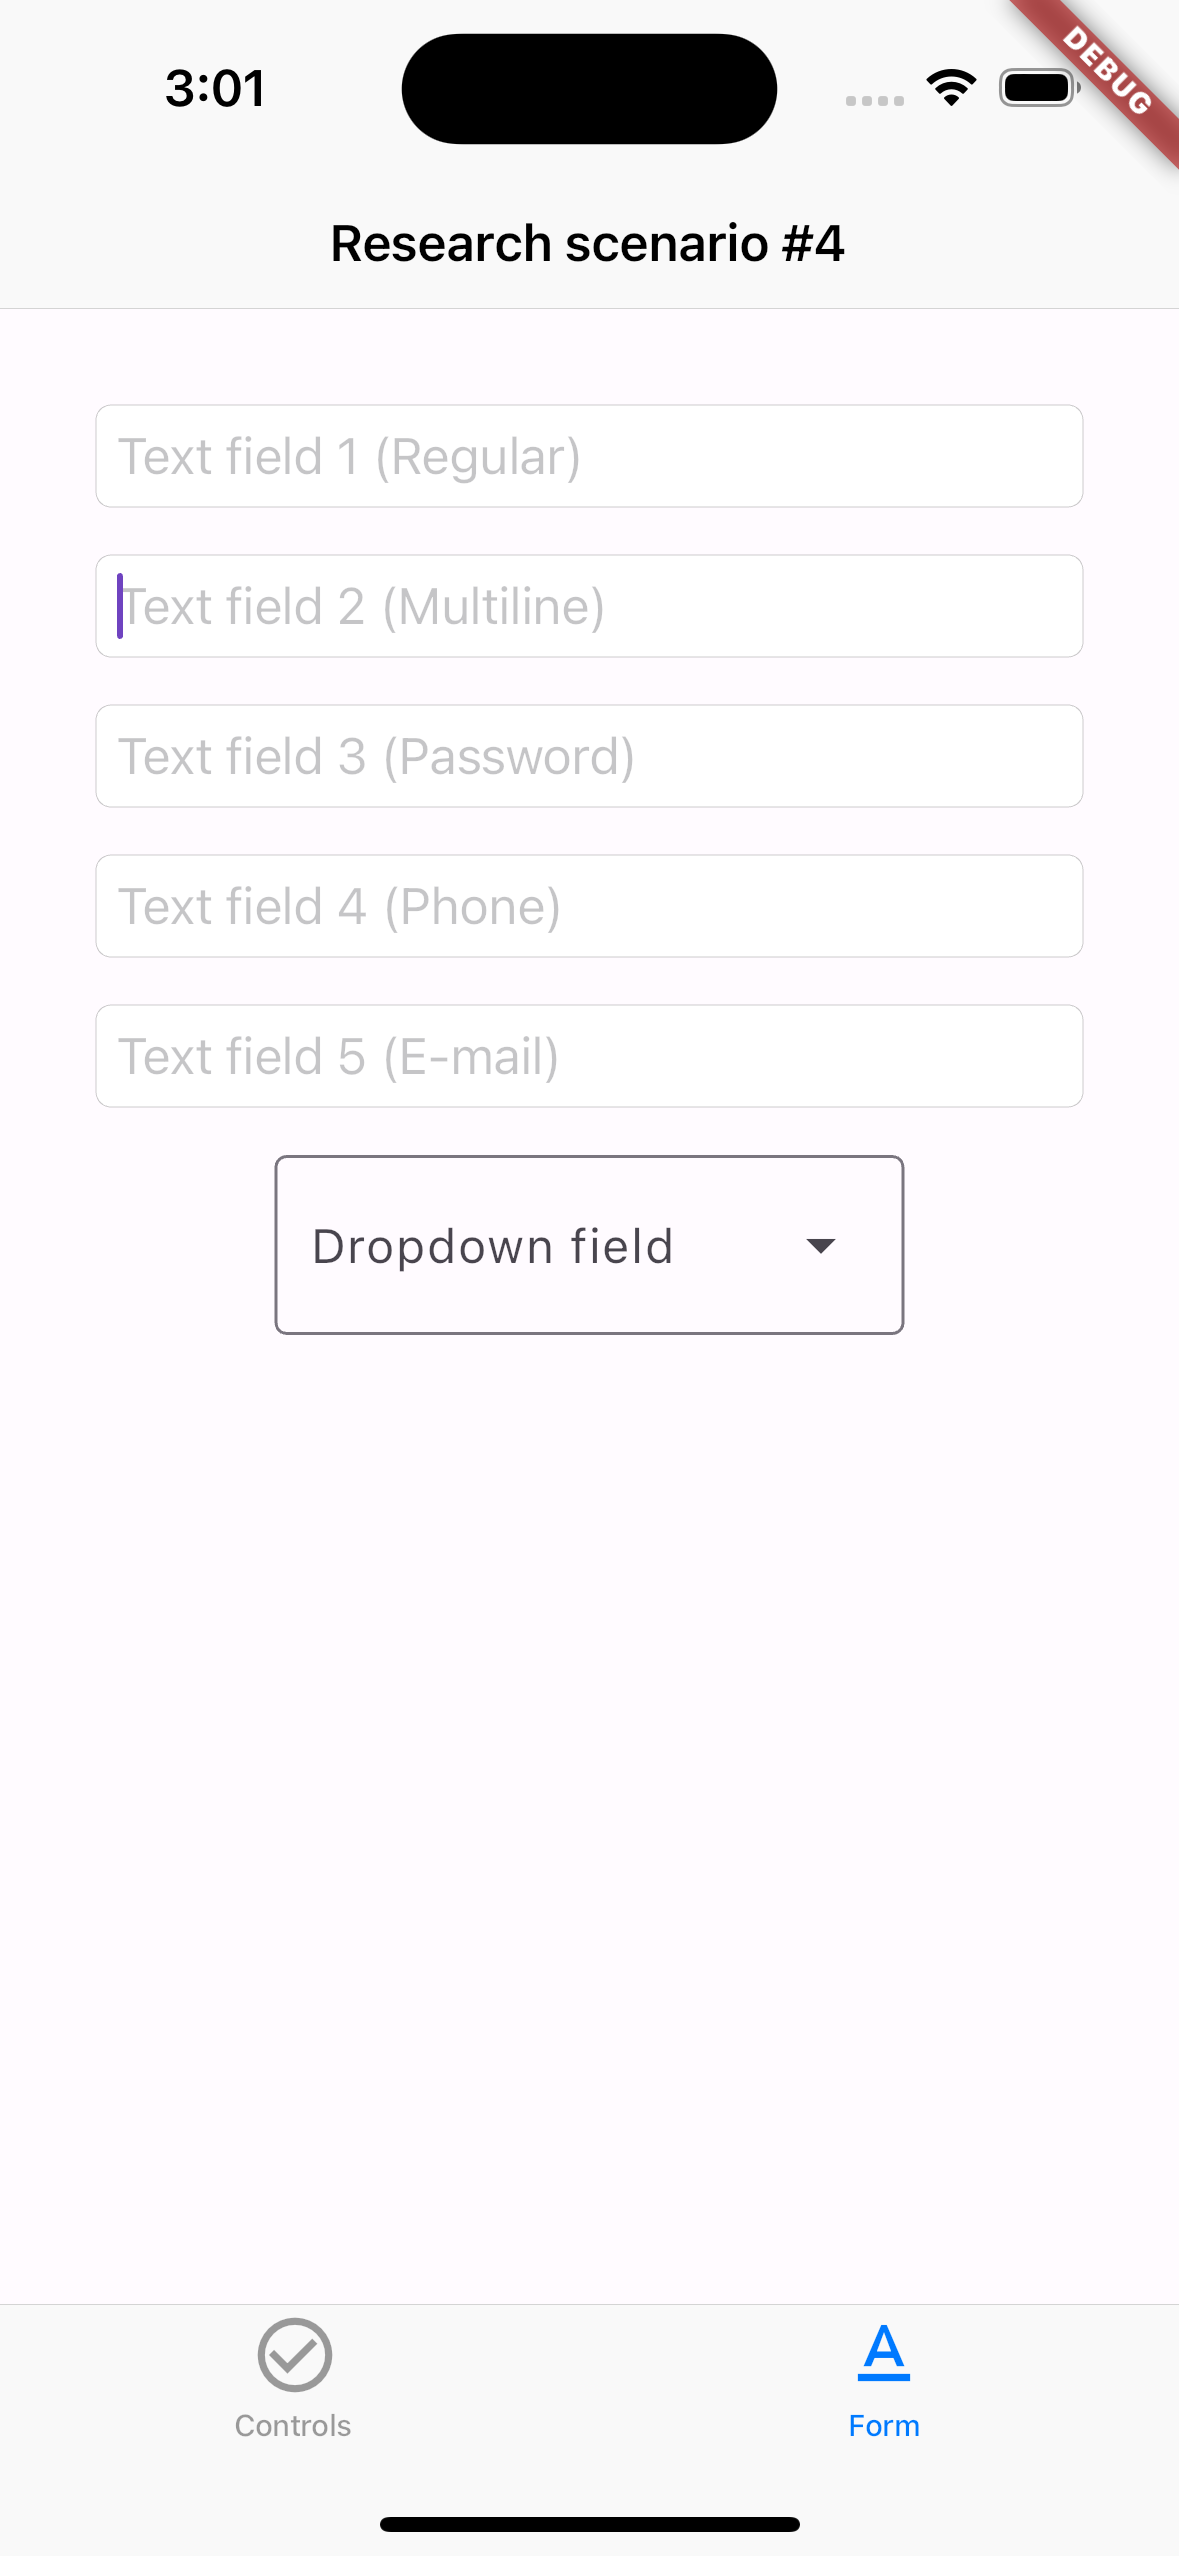
\includegraphics[height=50mm]{img/app4_3_flutter_ios}
    \caption{App 4 (3/3): Flutter iOS (Source: Own work)}
    \label{fig:app4_3_flutter_ios}
  \end{minipage}
\end{figure}

\begin{figure}[H]
  \begin{minipage}{.31\textwidth}
    \centering
    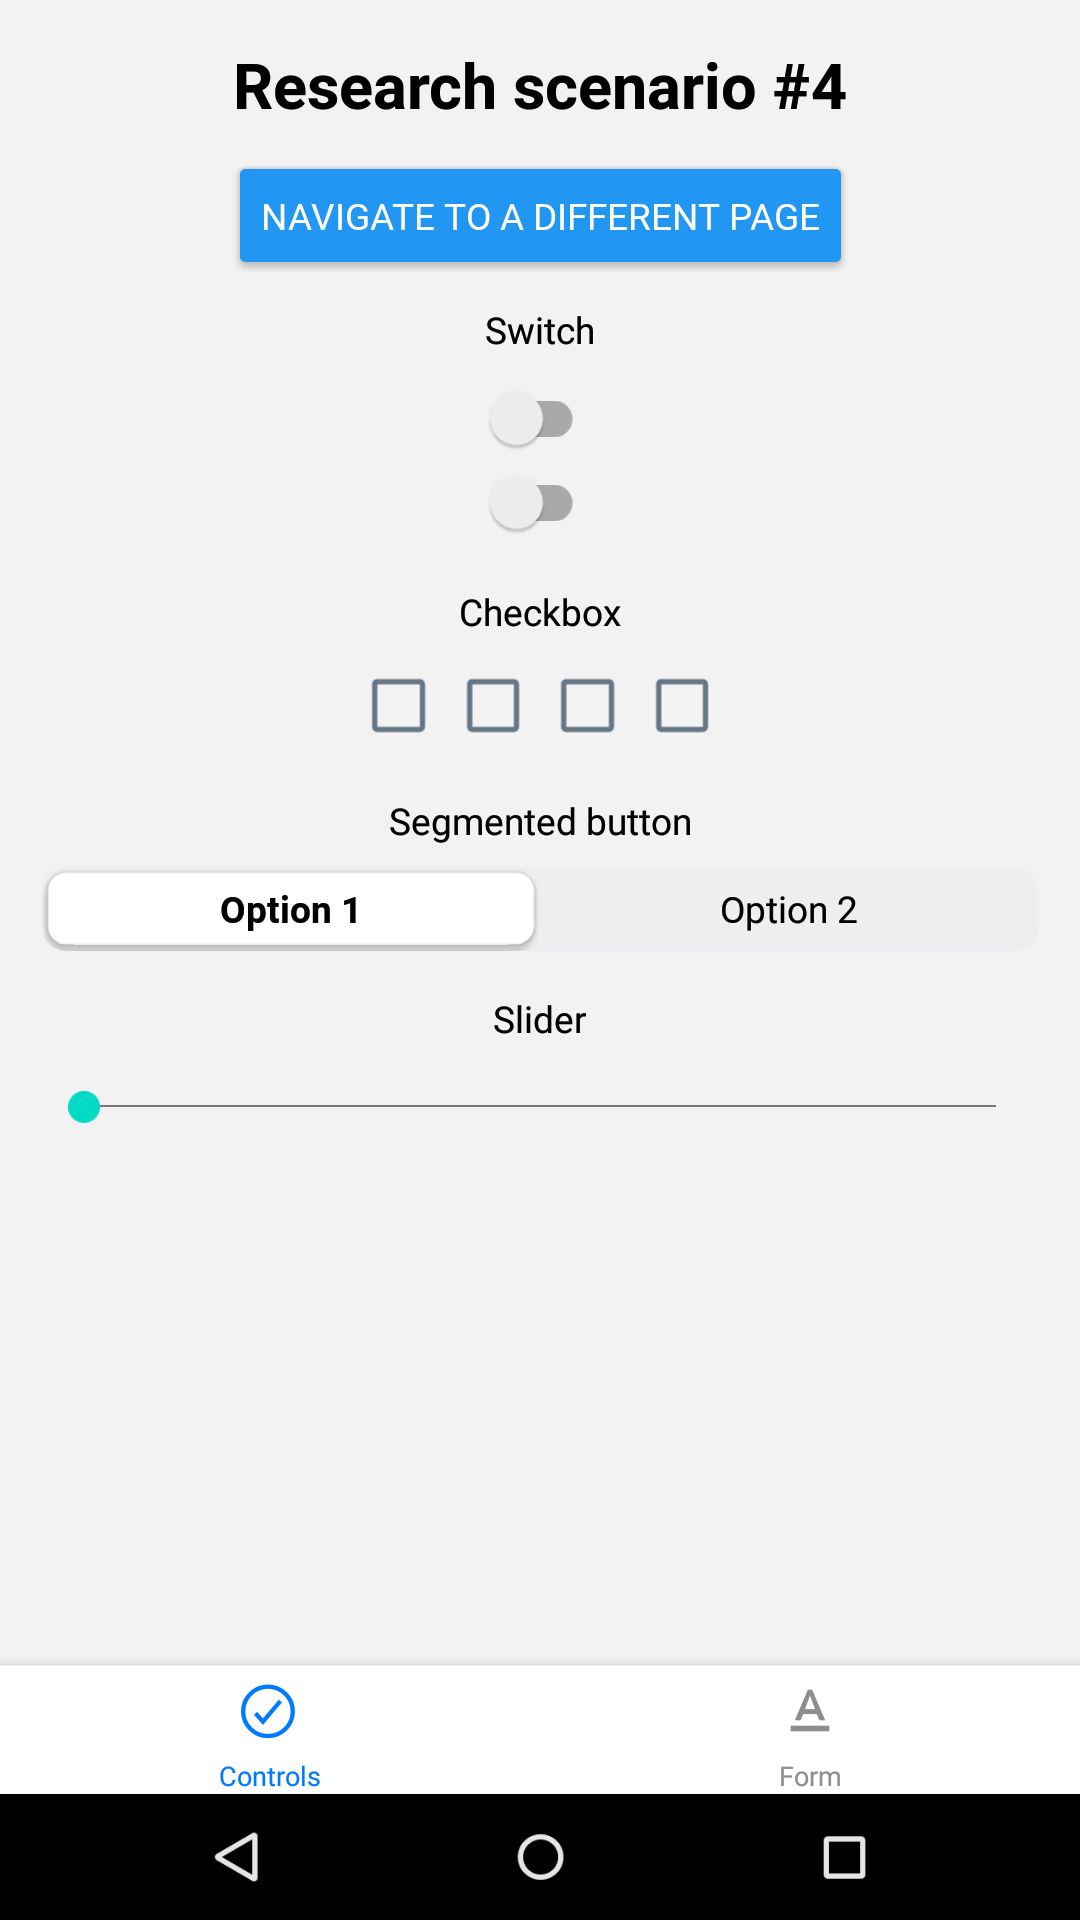
\includegraphics[height=50mm]{img/app4_1_rn_android}
    \caption{App 4 (1/3): React Native Android (Source: Own work)}
    \label{fig:app4_1_rn_android}
  \end{minipage}
  \hfill
  \begin{minipage}{.31\textwidth}
    \centering
    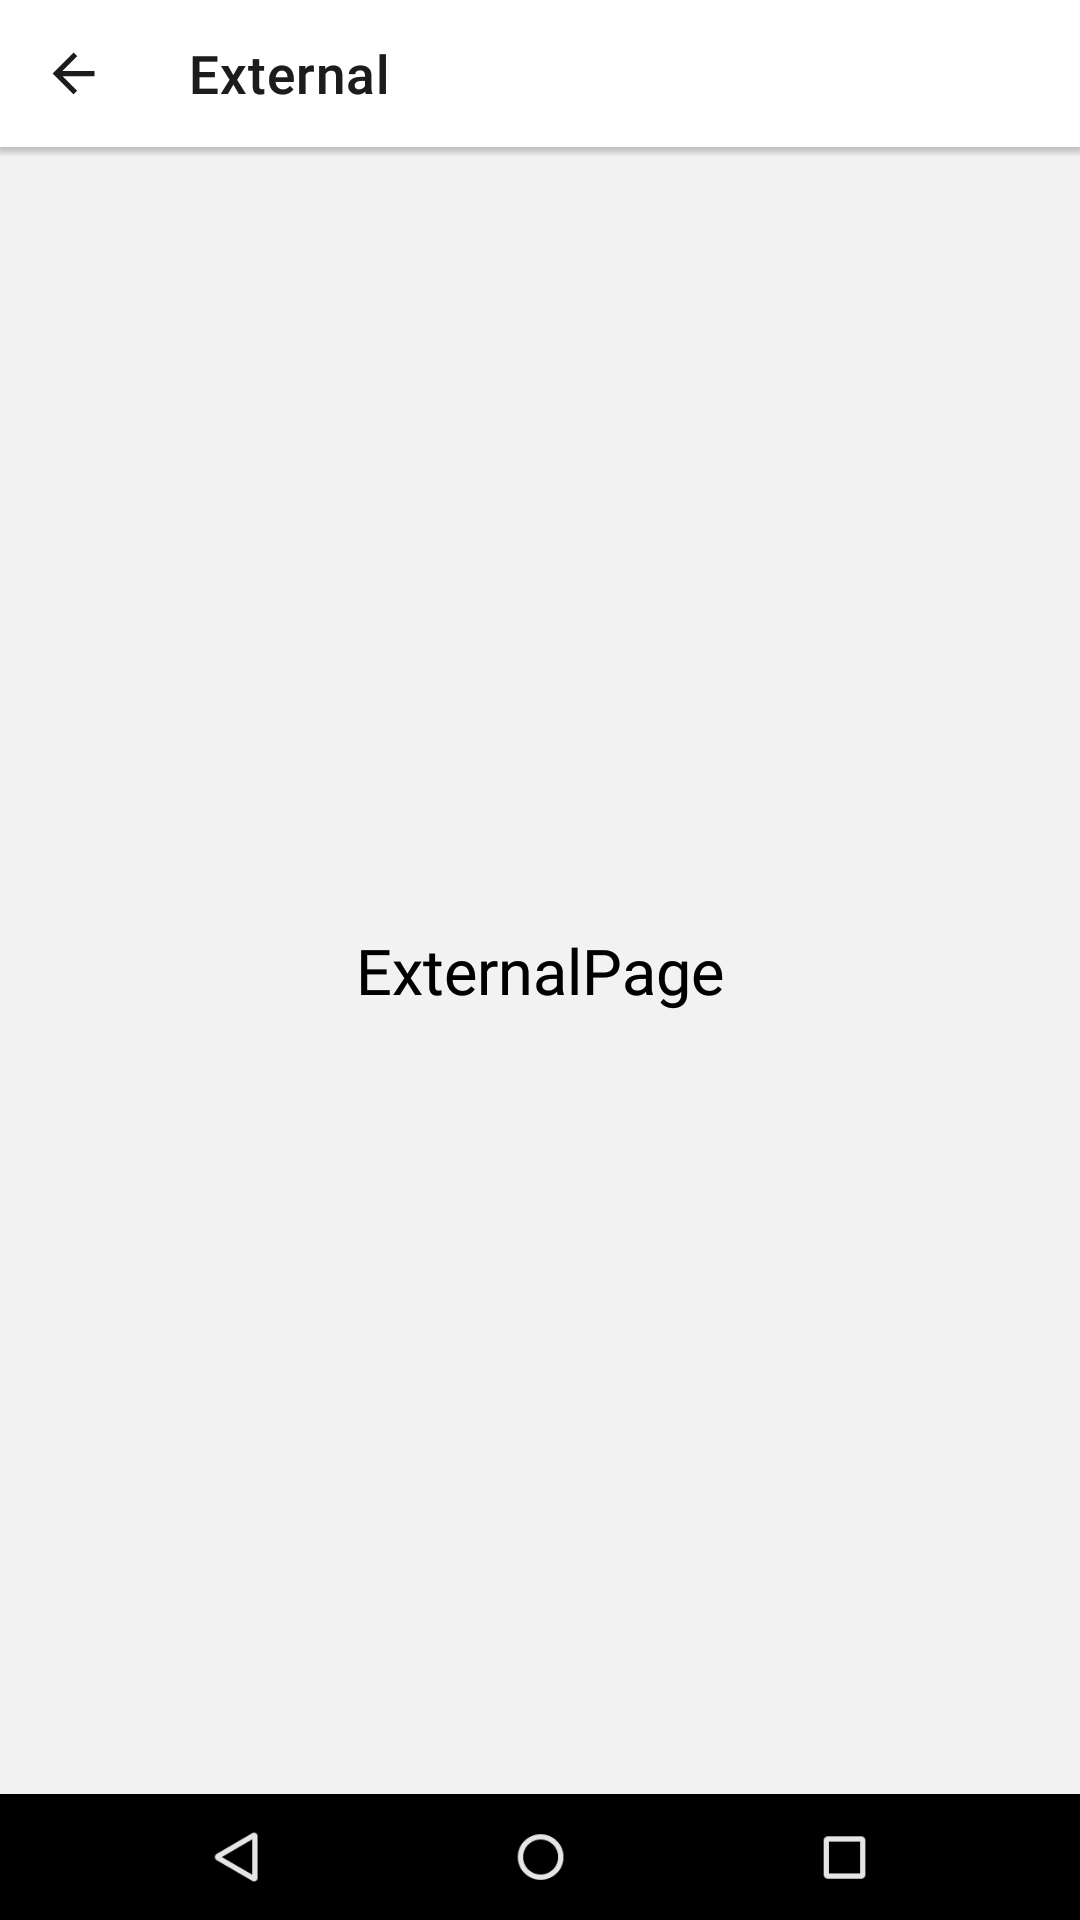
\includegraphics[height=50mm]{img/app4_2_rn_android}
    \caption{App 4 (2/3): React Native Android (Source: Own work)}
    \label{fig:app4_2_rn_android}
  \end{minipage}
  \hfill
  \begin{minipage}{.31\textwidth}
    \centering
    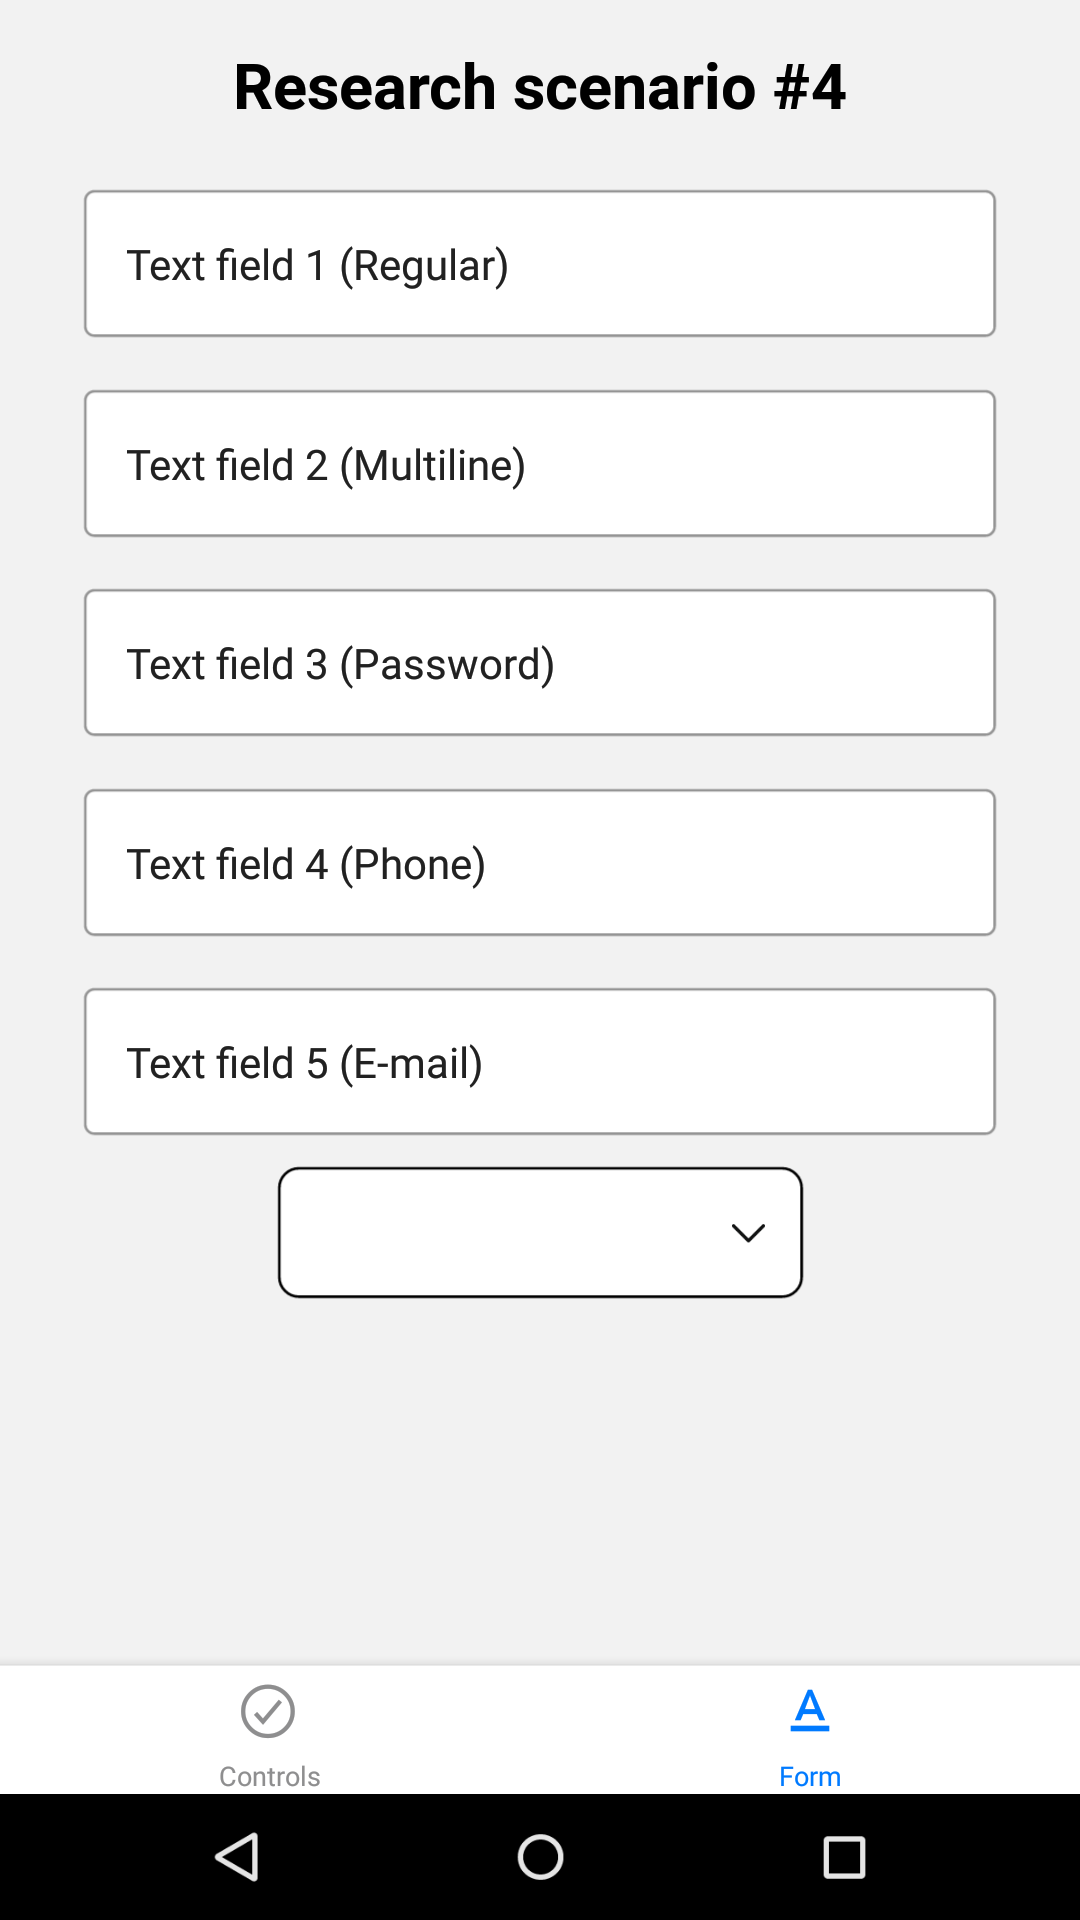
\includegraphics[height=50mm]{img/app4_3_rn_android}
    \caption{App 4 (3/3): React Native Android (Source: Own work)}
    \label{fig:app4_3_rn_android}
  \end{minipage}
\end{figure}

\begin{figure}[H]
  \begin{minipage}{.31\textwidth}
    \centering
    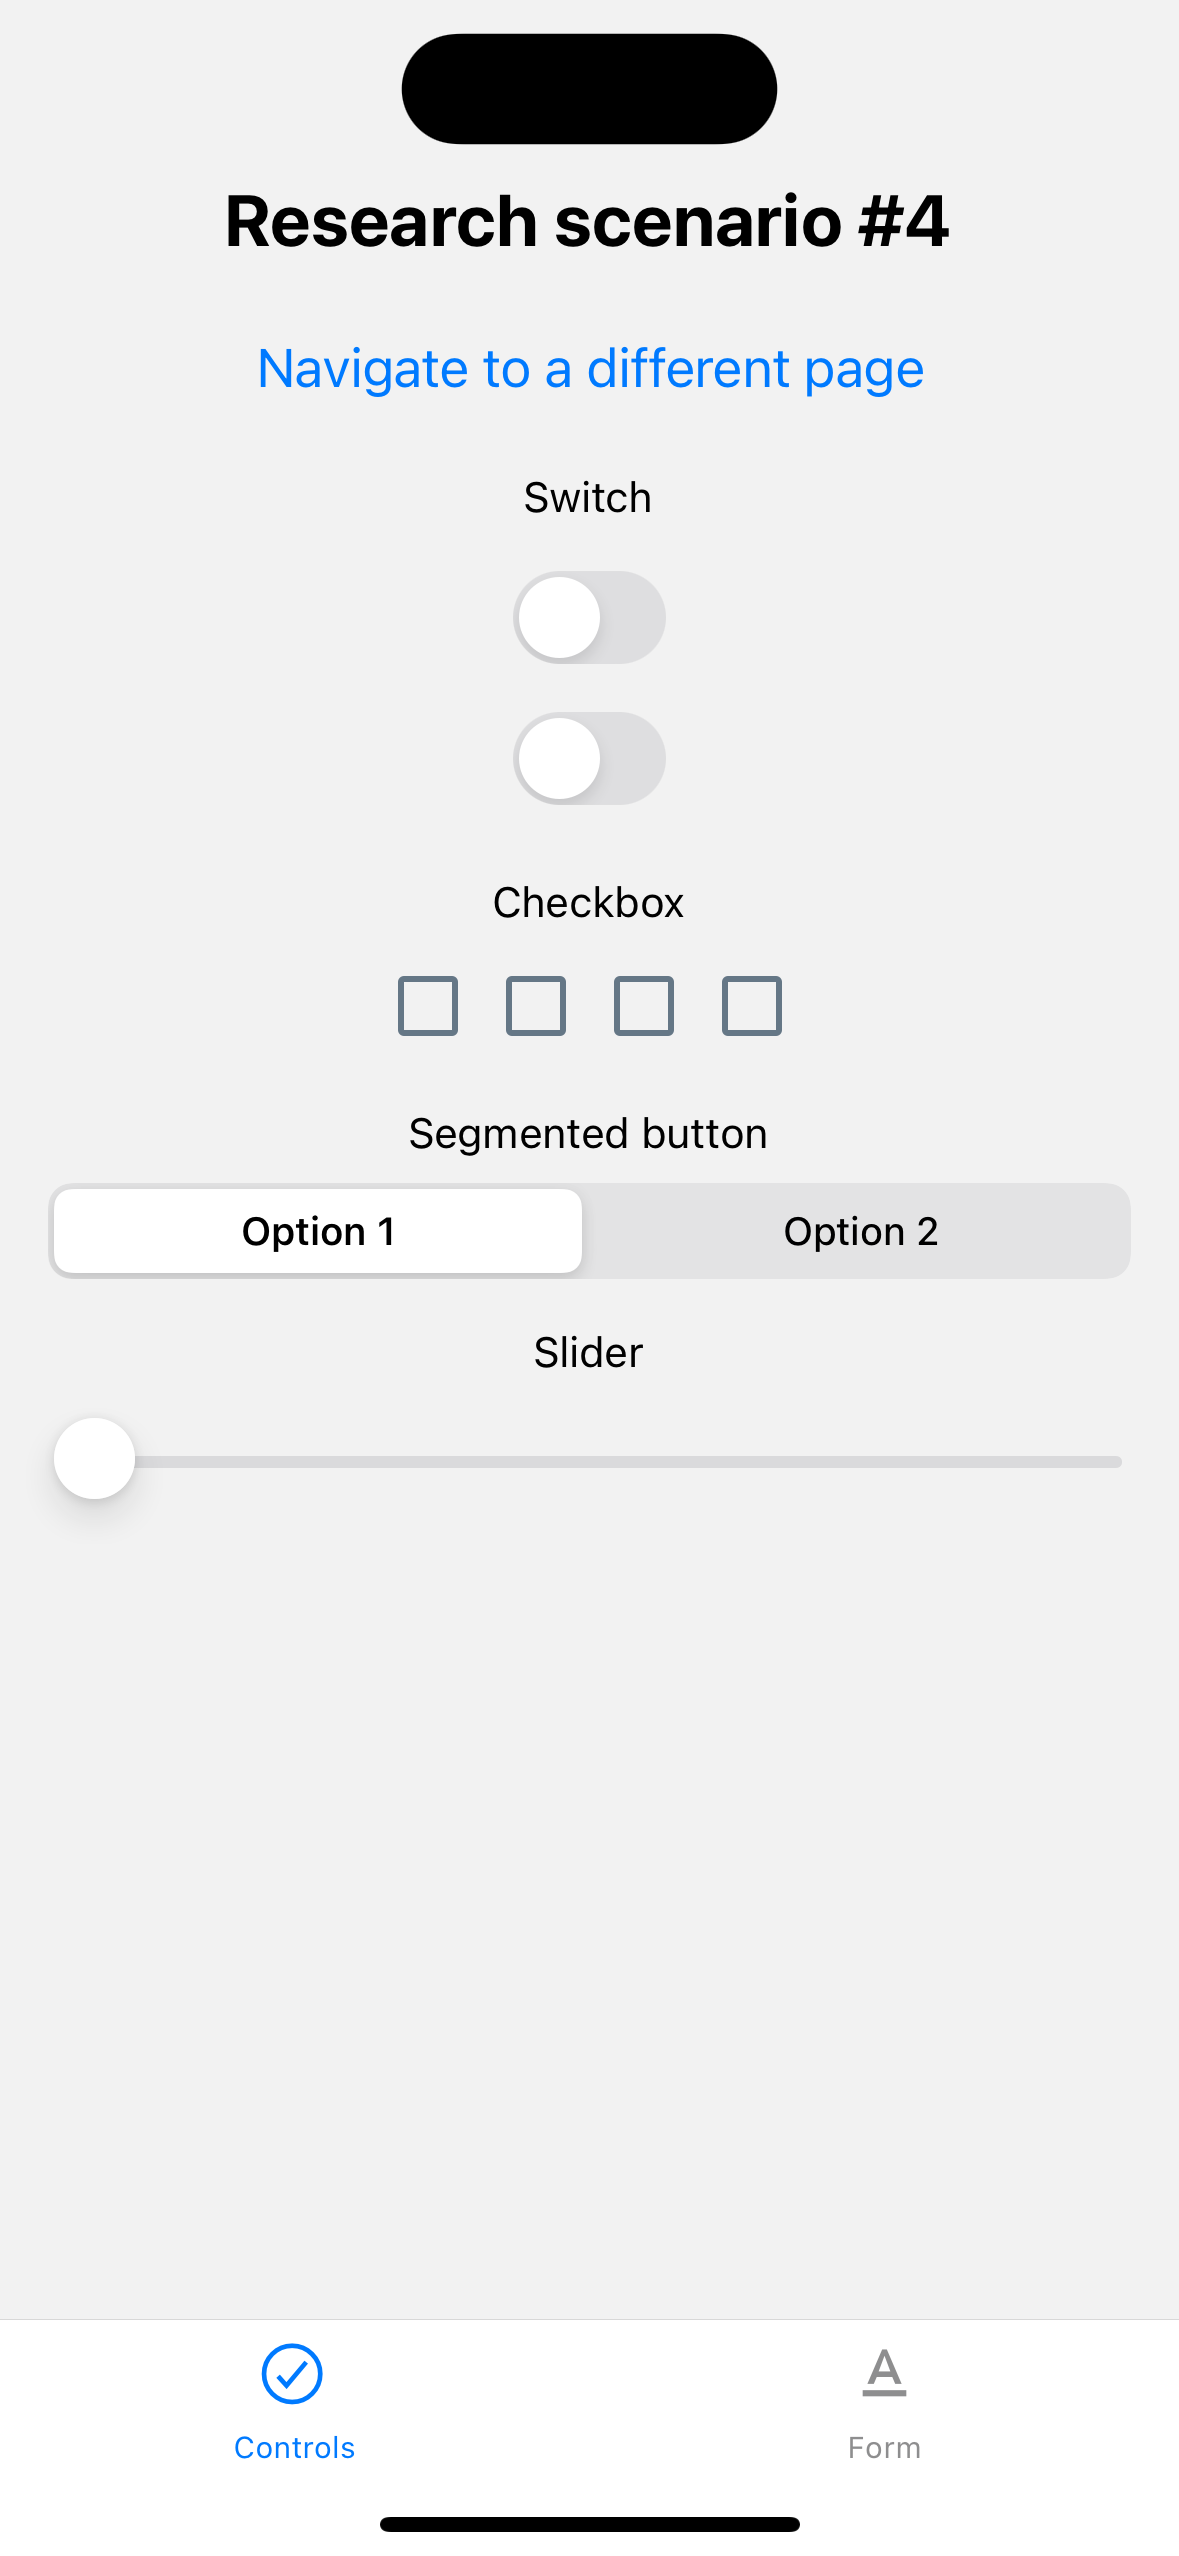
\includegraphics[height=50mm]{img/app4_1_rn_ios}
    \caption{App 4 (1/3): React Native iOS (Source: Own work)}
    \label{fig:app4_1_rn_ios}
  \end{minipage}
  \hfill
  \begin{minipage}{.31\textwidth}
    \centering
    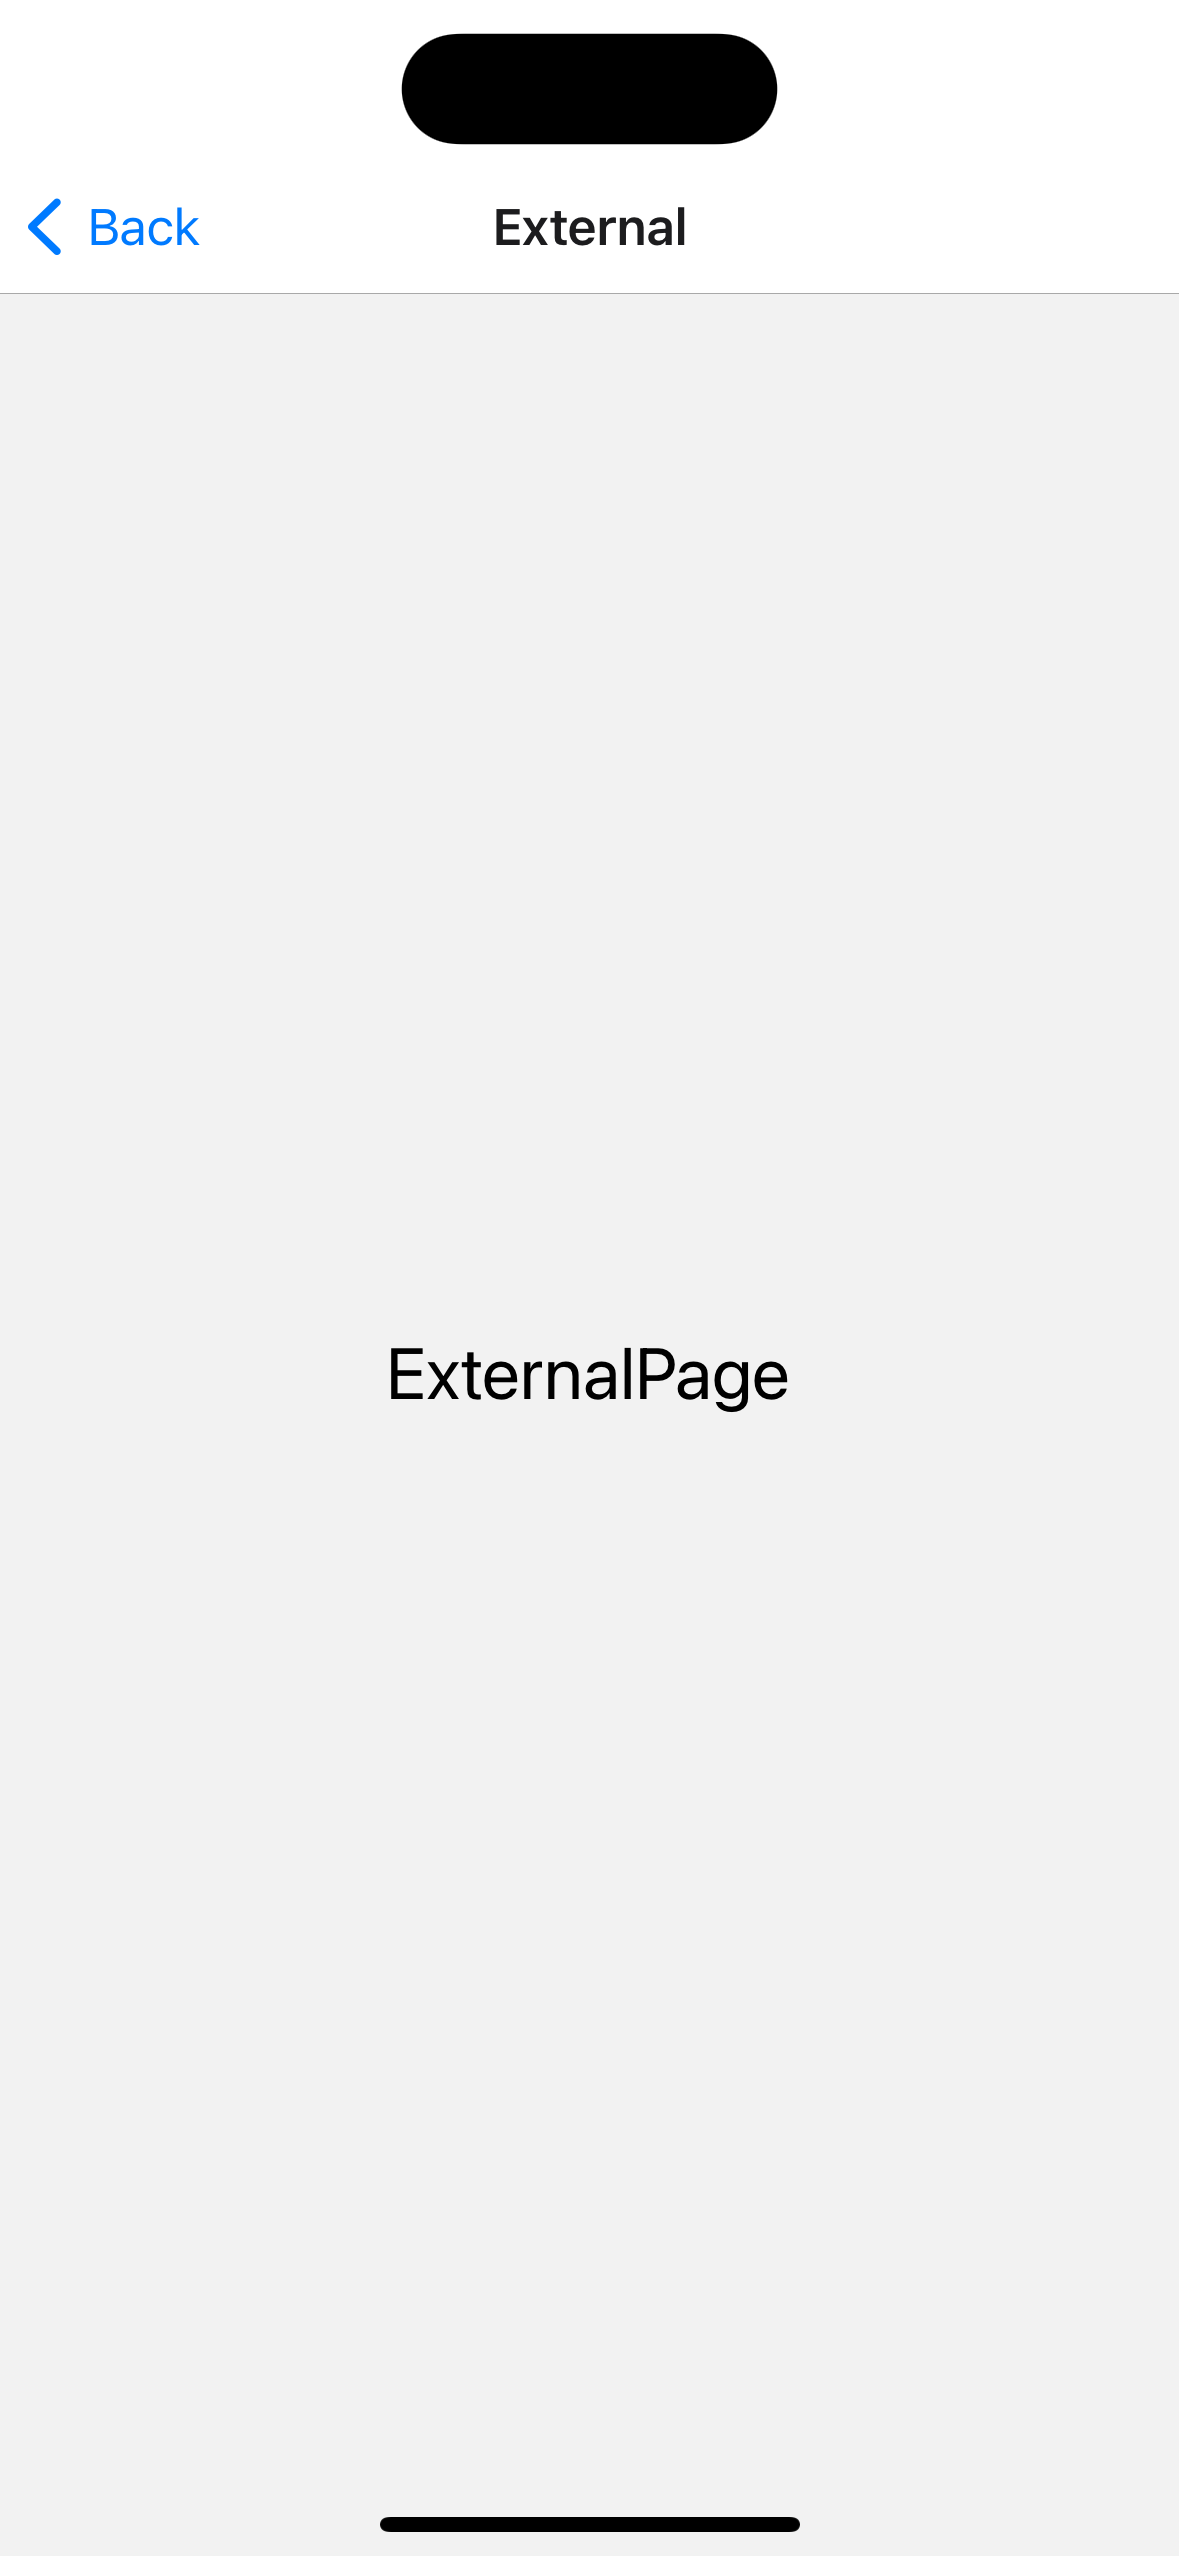
\includegraphics[height=50mm]{img/app4_2_rn_ios}
    \caption{App 4 (2/3): React Native iOS (Source: Own work)}
    \label{fig:app4_2_rn_ios}
  \end{minipage}
  \hfill
  \begin{minipage}{.31\textwidth}
    \centering
    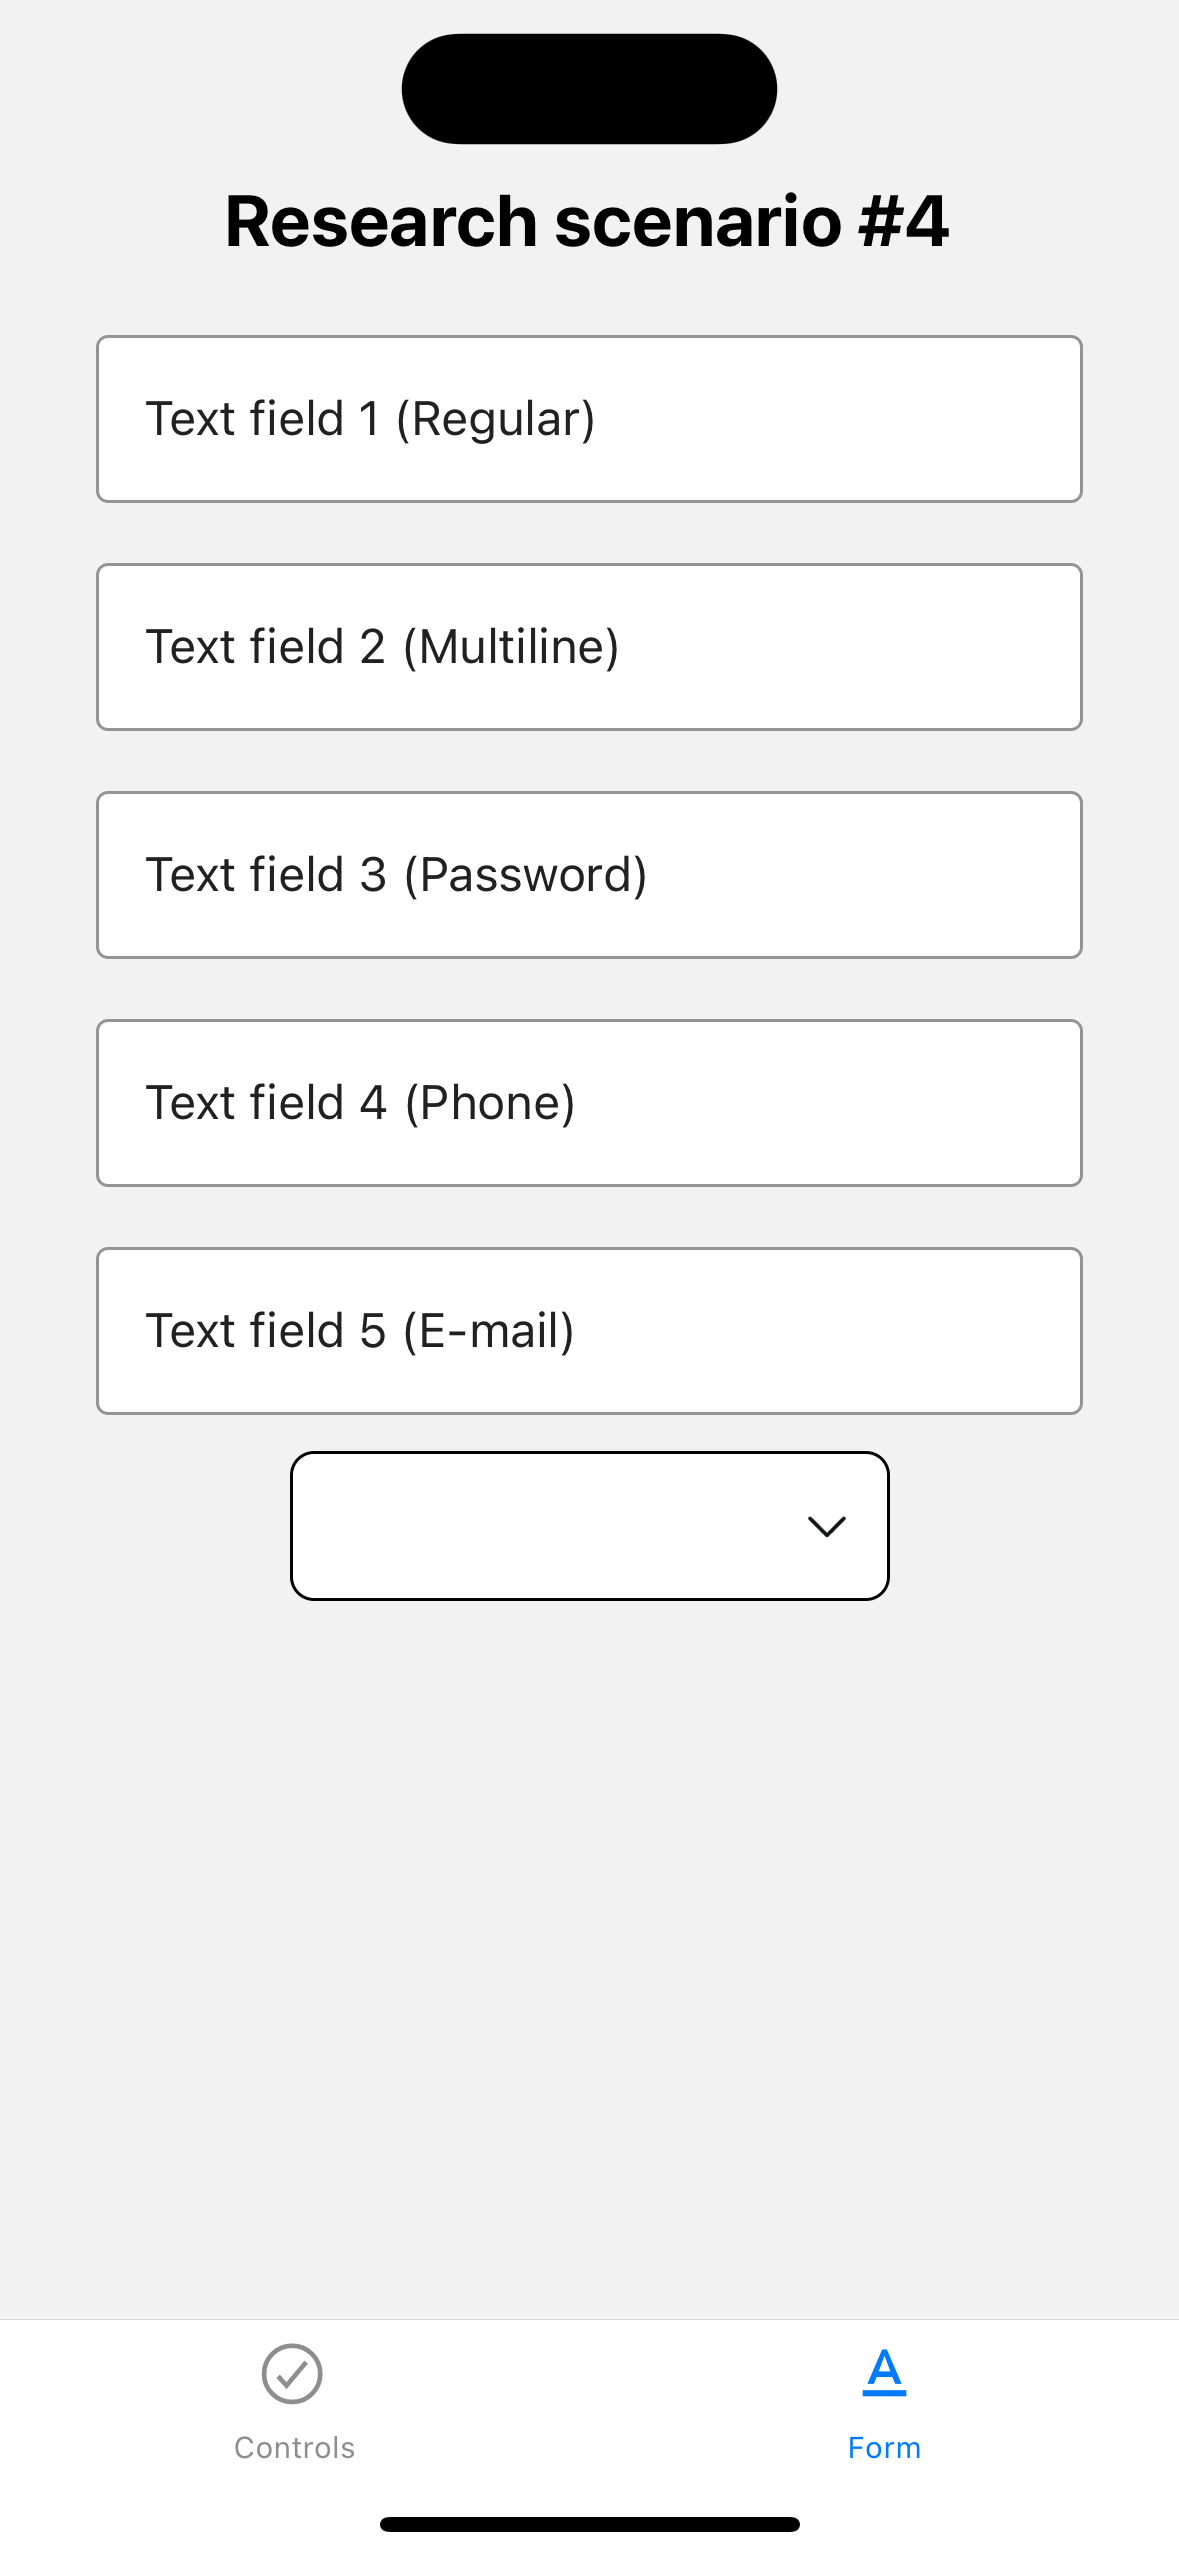
\includegraphics[height=50mm]{img/app4_3_rn_ios}
    \caption{App 4 (3/3): React Native iOS (Source: Own work)}
    \label{fig:app4_3_rn_ios}
  \end{minipage}
\end{figure}

\section{Key takeaways obtained during the implementation process}

Ease of development

Documentation

Native look (include material3!!)
